% First try
\documentclass[11pt,a4]{memoir}

%\usepackage{layouts}[2001/04/29]
\usepackage{url}
\usepackage{fixltx2e}
\usepackage{alltt}
\usepackage{graphicx}
\usepackage{chngpage}
\usepackage{amsmath}
\usepackage{listings}
\usepackage[usenames]{color}
\usepackage{setspace}
\usepackage{tabularx}
\usepackage{array}
\usepackage{multirow}
\usepackage{lscape}

%\usepackage{rotating}
%\usepackage{setspace}


\ifpdf
  \pdfoutput=1
  \usepackage[plainpages=false,pdfpagelabels,bookmarksnumbered]{hyperref}
  \usepackage{memhfixc}
\fi

\hypersetup{
    bookmarks=true,         % show bookmarks bar?
    unicode=false,          % non-Latin characters in Acrobat�s bookmarks
    pdftoolbar=true,        % show Acrobat�s toolbar?
    pdfmenubar=true,        % show Acrobat�s menu?
    pdffitwindow=true,      % page fit to window when opened
    pdftitle={OSCAR guide},    % title
    pdfauthor={Jerome Degallaix},     % author
    pdfsubject={A user guide for OSCAR},   % subject of the document
    pdfnewwindow=true,      % links in new window
    pdfkeywords={keywords}, % list of keywords
    colorlinks=true,       % false: boxed links; true: colored links
    linkcolor=red,          % color of internal links
    citecolor=green,        % color of links to bibliography
    filecolor=magenta,      % color of file links
    urlcolor=cyan           % color of external links
}

\renewcommand{\topfraction}{0.9}
    \renewcommand{\bottomfraction}{0.8}
    \setcounter{topnumber}{2}
    \setcounter{bottomnumber}{2}
    \setcounter{totalnumber}{4}
    \setcounter{dbltopnumber}{2}
    \renewcommand{\dbltopfraction}{0.9}
    \renewcommand{\textfraction}{0.07}
    \renewcommand{\floatpagefraction}{0.7}
    % floatpagefraction MUST be less than topfraction !!
\renewcommand{\dblfloatpagefraction}{0.7}






\begin{document}
\graphicspath{{Pics/pdf/}}
%\setcounter{lofdepth}{5}
%\setcounter{secnumdepth}{3}
\maxsecnumdepth{subsection}
\settocdepth{subsection}
\definecolor{OGreen}{rgb}{0,0.5,0}


\lstset{language=Matlab,
        basicstyle=\footnotesize,
        keywordstyle=\color{black},
        commentstyle=\color{OGreen},
        stringstyle=\normalfont,
        columns= flexible}


\begin{titlingpage}
    \setlength\hoffset{-52pt}
    \setlength\voffset{-120pt}
    \begin{figure}[!ht]
    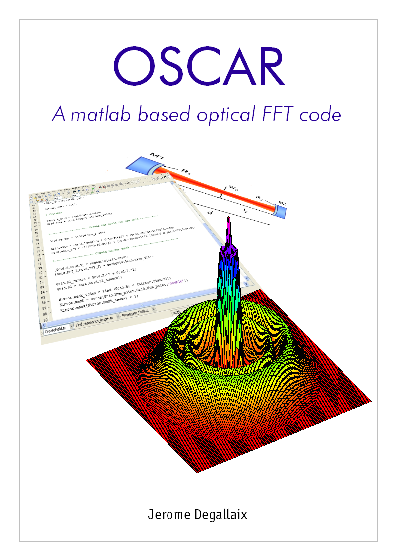
\includegraphics[width=1.47\textwidth]{title3.pdf}
    \end{figure}
\end{titlingpage}

\frontmatter

\pagestyle{empty}
\vspace*{4cm}
  \rule{\textwidth}{0.5pt}
\begin{flushright}
    \HUGE\textsf{OSCAR}\par
    \Large\textsf{The Non-Definitive Guide}
\end{flushright}
\vspace*{\fill}

\clearpage

\vspace*{2cm}

\begin{tabular}{p{5cm}p{5cm}}
  First edition & July 2008 \\
  Second edition & October 2008 \\
  Third edition & April 2009 \\
  Fourth edition & January 2010 \\
  Fifth edition & January 2012 \\
  Sixth edition & June 2012 \\
  Seventh edition & January 2013 \\
  Eight edition & September 2013 \\
  Ninth edition & December 2013 \\
  Tenth edition & July 2014 \\
  Eleventh edition & December 2014 \\
  Twelfth edition & September 2016 \\
  Thirteenth edition & August 2019 \\
\end{tabular}


\begingroup
\footnotesize

\vspace*{\fill}
\noindent OSCAR, the Matlab code, this documentation as well as the examples were written by:
\begin{tabular}{l}
Jerome Degallaix \\
Laboratoire des Mat\'eriaux Avanc\'es (LMA)\\
Universit\'e Claude Bernard Lyon I \\
7, Avenue Pierre de Coubertin \\
69622 Villeurbanne \\
France \\
\end{tabular}
\vspace*{\baselineskip}

\noindent THE SOFTWARE AND DOCUMENTATION IS PROVIDED AS IS WITHOUT ANY WARRANTY
OF ANY KIND.\\

\noindent MATLAB is a trademark of MathWorks Inc., MA, USA.

\endgroup

\clearpage

\vspace*{5cm}
OSCAR is an optical FFT code used to calculate the steady state optical field circulating in Fabry-Perot cavities. The code can integrate non-spherical mirrors and any arbitrary input fields. Typical applications for OSCAR have been: calculation of thermal lensing effect and calculation of diffraction loss and cavity eigenmodes for arbitrary beam shapes. One great advantage of OSCAR is the simplicity and flexibility of the code, everyone with only minimal knowledge of Matlab can easily modified OSCAR code to suit specific purposes.\\

If you find a bug when using OSCAR, please feel free to contact the author. Do not hesitate also to report any unclear part from this manual or from the code itself. Of course, I am also open to suggestions and possible improvements.
%\vspace*{\fill}

\clearpage


\tableofcontents


\mainmatter



\chapter{Principle of the FFT code}
\pagestyle{headings}

In this chapter, we detail the two main steps used to propagate an electric field in a Fabry-Perot cavity. Firstly we will understand how the propagation of any arbitrary electric fields can be simulated using a Fourier transform. And secondly, we will see how any wavefront distortions encountered by the electric fields can be included in the numerical simulations. Whenever possible some simple Matlab codes are presented to show the numerical implementation of the algorithm. For clarity, the snippets of code are \textbf{not} optimised.

\section{Why OSCAR ?}

OSCAR is a FFT code which is able to simulate Fabry Perot cavities with arbitrary mirror profiles. One of the key features of OSCAR is the possibility to easily modify the code to suit the user purpose. For this reason, OSCAR is written with the Matlab language, one can import/export files (mirror maps or cavity eigenmodes profile for example), create a ring cavity, create batch file or plot 2D optical field with little programming skill\footnote{The code  can also be useable with the free Matlab-alternatives such as Sci-Lab or Octave with only minor modifications. Even a minimal Python version also exists.}. The fact that I encourage everyone to understand the code of OSCAR in details and to also modify it, is the main reason for this lengthy manual.

\subsection{Origin of OSCAR}

I started writing and using OSCAR during my PhD where I had to simulate the effects of thermal lensing in high optical power cavities. Wavefront distortions induced by the optical absorption have seldom pure spherical profiles, which means it is delicate to quantify thermal lensing effects with modal expansion code (but still possible).
To simulate the effects of the optical absorption on the mirror, I was using the FEM package Ansys which can calculate the temperature distribution inside the mirror substrate or the surface deformations due to the absorption of a Gaussian beam. From the Ansys results, it is straight forward to calculate the wavefront distortion induced by thermal lensing. However, at this stage, I was facing a problem, how can I estimate the effects of the thermal lens if it has to be inserted in a Fabry-Perot cavity ? how much the circulating power will decrease ? Will the cavity optical modes keep their Gaussian profiles ? I needed an optical simulation tool which can be used with any arbitrary mirror profile. OSCAR was born. For the inquisitive reader, the name OSCAR is the acronym of Optical Simulation Containing Ansys Results.

The first version of OSCAR was written with the software IGOR. This code was then translated to Matlab and used to calculate diffraction losses by my UWA colleague Pablo Barriga. Finally, I re-wrote and optimised the Matlab code to substantially decrease the OSCAR computational time. During the year 2011, OSCAR was totally revamped using the Oriented Object capability of Matlab giving rise to the Version 3.0.

\subsection{Which results could I get from OSCAR ?}

OSCAR is a versatile tool to simulate Fabry Perot cavities. The following is a (non-exhaustive) list of the results which can be obtained with OSCAR:
\begin{itemize}
  \item calculate the Gouy phase shift between higher order optical modes. It may be useful for flat beams for example, where no analytical calculations of the Gouy phase shift has been derived yet (as far as I know)
  \item calculate the coupling loss between the input beam and the cavity eigenmodes in case mode mismatching
  \item calculate the circulating beam (intensity and profile) inside the cavity, which may be different from the eigenmodes if the cavity has a low finesse
  \item calculate diffraction loss and eigenmodes of cavity for arbitrary mirror profiles
  \item calculate the effects of imperfect optics, due to the micro-roughness of the coating surface or thermal lens inside the substrate of the mirrors.
\end{itemize}

Even more complicated configuration could also be simulated such as dual recycled Michelson with Fabry-Perot arm cavities (topology of advanced laser gravitational wave detectors). However the code is more complex and lacking exhaustive documentation, but it is available on demand.

\subsection{What OSCAR is not for}

OSCAR is designed to simulate anything which can be derived from the steady state, classical, optical field circulating inside a Fabry-Perot cavity. It means OSCAR does not take into account radiation pressure or quantum effect (no shot noise calculations).

\section{Propagation of an optical field}
\label{sec1.2}

In this section we will see how it is possible to propagate a coherent electric field, i.e. a laser beam, with the help of the Fourier transform. The principle of the FFT optical propagation code is similar to the Fourier transformation method used to calculate the response of a linear system to an arbitrary function $f_i(t)$. The function $f_i(t)$ is expressed as a continuous superposition of harmonic functions of different frequencies $\nu$:
\begin{equation}
 f_i(t) = \int_{-\infty}^{\infty} \widetilde{f_i}(\nu) \exp(2\pi j \nu t) d\nu
\label{eq1:four}
\end{equation}

\noindent Where $\widetilde{f_i}$ is the Fourier transform of the function $f_i$. The function $ t\rightarrow \exp(2\pi j \nu t)$ is the harmonic function of frequency $\nu$. These are the basic functions used to expand $f_i$. If the response of the system is known for each elementary harmonic function $\exp(2\pi j \nu t)$, the response of the system to the input $f_i$ can be derived using three steps. First step, the function $f_i$ is expanded in the sum of basic harmonic functions by doing a Fourier transformation. Second step the response of the system to each harmonic function is calculated. This is done simply by a multiplication in the frequency domain. Finally, third step, the output of the system to the input $f_i$ is derived by doing the inverse Fourier transformation of the output harmonic functions (step similar to the equation \ref{eq1:four}).\\

The FFT optical propagation code follows exactly the principle described in the previous paragraph. In this case the elementary functions are plane waves of different spatial frequencies.

\subsection{Propagation of a plane wave}

We can first understand how to propagate of an elementary plane wave $u$ through free space. At $z = 0$, $u$ can be simply written:

\begin{equation}
u(x,y,0) = \exp(-j k_x x - j k_y y)
\label{eq1:uel}
\end{equation}

\noindent with $k_{x/y}$ the propagation constant along the $x/y$ axis. Equation (\ref{eq1:uel}) can also be written:
\begin{equation}
u(x,y,0) = \exp(-j 2 \pi (\nu_x x + \nu_y y)) \mbox{ with } \nu_x = k_x/(2 \pi) \mbox{ and } \nu_y = k_y/(2 \pi)
\label{eq1:uel2}
\end{equation}

If $u$ is written as shown in equation (\ref{eq1:uel2}), it is easy to recognise $u$ as a harmonic function of two variables $(x,y)$ with respective spatial frequencies \footnote{The term spatial frequency $\nu$ must be understood as the number of wavelength per unit of length $\nu = 1/\lambda = k / 2\pi$} $(\nu_x,\nu_y)$. If we propagate $u$ along the z axis over a distance d:
\begin{equation}
u(x,y,d) = \exp(-j k_x x - j k_y y - j k_z d)
\label{eq1:uel3}
\end{equation}

\begin{figure}
\begin{center}
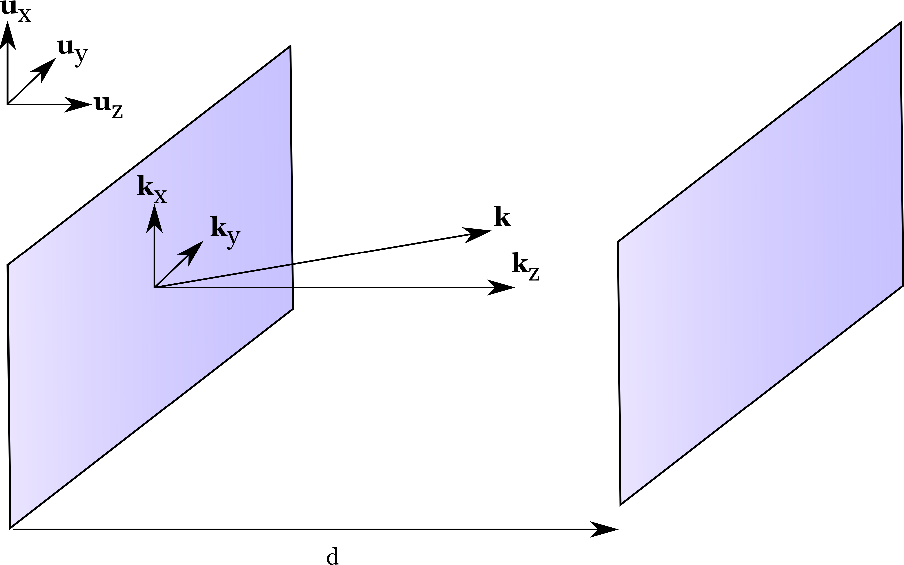
\includegraphics[width = 0.80\textwidth]{Planewave.pdf}
\end{center}
\caption{\label{fig1:plane} Propagation of a plane wave along the z axis.}
\end{figure}


\noindent with $k =  (k_x^2 + k_y^2 + k_z^2)^{\frac{1}{2}} = 2 \pi / \lambda $. If we suppose the wave to be traveling in a direction close to the z axis (paraxial approximation) as shown in figure \ref{fig1:plane}, $k_z \gg k_x$ and $k_z \gg k_y$, then $k_z$ can be written as:
\begin{eqnarray}
k_z = (k^2 - k_x^2 - k_y^2)^{\frac{1}{2}} & \simeq & k - \frac{(k_x^2 + k_y^2)}{2 k } \label{eq4:uel4a}\\
& \simeq & k - \lambda \pi (\nu_x^2 + \nu_y^2)
\label{eq1:uel4}
\end{eqnarray}

\noindent So we can rewrite equation (\ref{eq1:uel3}) as:
\begin{equation}
u(x,y,d) = u(x,y,0) \exp(-j (k - \lambda \pi (\nu_x^2 + \nu_y^2))d)
\label{eq1:uel5}
\end{equation}

The equation (\ref{eq1:uel5}) is the foundation of the FFT propagation code. It tells us that the propagation of a plane wave along the z axis over a distance $d$ can simply be represented by a phase shift. The function $ d\rightarrow \exp(-j (k - \lambda \pi (\nu_x^2 + \nu_y^2))d)$ could also be seen as the propagation operator for an input plane wave traveling a distance $d$ under the paraxial approximation. The term $\exp(-j (k d))$ represents the phase shift of a plane wave propagating along the z axis and the term $ \exp (j \lambda \pi (\nu_x^2 + \nu_y^2)d)$ adds a phase correction to take into account the fact that the wave propagates with a small angle with respect to the z axis\footnote{The angle $\theta_x$ between the direction of propagation and the x axis is $\theta_x = sin^{-1}(k_x/k)$. In the case of small angles, it is simply $\theta_x = \lambda \nu_x$}.\\


We noticed in equation (\ref{eq1:uel2}), that the elementary plan wave $u(x,y,0)$ can also be seen an harmonic function with spatial frequency $\nu_x$ and $\nu_y$. To keep the analogy developed in the introduction of this chapter with the classical time domain Fourier transform, the plane wave is equivalent to the elementary harmonic function $t\rightarrow \exp(2\pi j \nu t)$ of frequency $\nu$. Since we know how to propagate a plane wave, we understand now how it may be possible to propagate any arbitrary field if we can manage to expand it as a superposition of elementary plane waves.

\subsection{Propagation of an arbitrary field}

Equation (\ref{eq1:uel5}) tells us how to propagate a plane wave. So to propagate any arbitrary electric fields $E$, we need to know how to expand the electric field onto the set of plane waves $\exp(-j 2 \pi (\nu_x x + \nu_y y))$. We would like to find $\widetilde{E}(\nu_x,\nu_y)$ such as:

\begin{equation}
 E(x,y) = \int_{-\infty}^{\infty} \int_{-\infty}^{\infty} \widetilde{E}(\nu_x,\nu_y) \exp(-j 2\pi (\nu_x x + \nu_y y)) d\nu_x d\nu_y
\label{eq4:uel6}
\end{equation}

With $\widetilde{E}(\nu_x,\nu_y)$ the complex amplitude of the component of the field $E$ with spatial frequency $(\nu_x,\nu_y)$. We recognise equation (\ref{eq4:uel6}) as an inverse 2D Fourier transform\footnote{In fact, if we respect the convention found in signal processing technique, equation (\ref{eq4:uel6}) is not an inverse Fourier transform but a Fourier transform\cite{Sig_proc}. It is not tragic, since we will stay consistent with the convention presented here.}. Using the properties of the Fourier transform\cite{Fourier_trans} we deduce the expression for $\widetilde{E}(\nu_x,\nu_y)$:

\begin{equation}
  \widetilde{E}(\nu_x,\nu_y) = \int_{-\infty}^{\infty} \int_{-\infty}^{\infty} E(x,y) \exp(j 2\pi (\nu_x x + \nu_y y)) dx dy
\label{eq4:uel7}
\end{equation}

Combining equations (\ref{eq1:uel5}), (\ref{eq4:uel6}) and (\ref{eq4:uel7}) , we know how to propagate in free space a transverse electric field $E$ from $z = 0$ to $z = d$. To calculate the resulting field after the propagation, three steps are required:
\begin{enumerate}

\item Decomposition of the field $E(x,y,0)$ into a sum of elementary plane waves. Mathematically, this step represents a 2D Fourier transformation.

\begin{equation}
 \widetilde{E}(\nu_x,\nu_y,0) = \int_{-\infty}^{\infty} \int_{-\infty}^{\infty} E(x,y,0) \exp(j 2\pi (\nu_x x + \nu_y y)) dx dy
\label{eq1:uel10}
\end{equation}

\item Propagation of each plane waves, which is equivalent of adding a phase shift in the frequency domain.


\begin{equation}
 \widetilde{E}(\nu_x,\nu_y,d) =  \widetilde{E}(\nu_x,\nu_y,0) \exp(-j (k - \lambda \pi (\nu_x^2 + \nu_y^2))d)
\label{eq1:uel11}
\end{equation}

\item Recomposition of the electric field from the propagated plane waves. This step is in fact an inverse Fourier transformation.

\begin{equation}
 E(x,y,d) = \int_{-\infty}^{\infty} \int_{-\infty}^{\infty}  \widetilde{E}(\nu_x,\nu_y,d) \exp(- j 2\pi (\nu_x x + \nu_y y)) d\nu_x d\nu_y
\label{eq1:uel12}
\end{equation}
\end{enumerate}


\subsection{My first Matlab FFT code}

There is an essential point to realize before implementing the three analytical steps described in the previous section. The computer does not deal with continuous electrical fields which means all the data fields have to be discretized. For example the amplitude of a Gaussian beam will be represented by a square matrix (called also grid later), each points of the matrix (called also pixel for convenience) will represent the amplitude of the Gaussian beam at a defined location. A 2D plot of such a matrix is shown in the top left corner of the figure \ref{fig1:FFT}.

Practically, the discretization process is governed by the choice of 2 parameters: the physical size represented by the matrix and the number of points in the matrix. For example, to discretize a laser beam with a beam radius of 1~cm we can use a matrix of size $128 \times 128$ representing an area of 10~cm by 10~cm. This example can be implemented in Matlab in a straight forward way as shown in the listing \ref{lis1:start1}.

\begin{lstlisting}[float=tp,caption=Discretization of a Gaussian beam\label{lis1:start1},frame=lines]
Grid.Num_point = 128;                                % Number of point in one side the grid
Grid.Length = 0.10;                                  % Physical dimension of the grid in meter
Grid.step = Grid.Length/Grid.Num_point;              % Physical size of one pixel of the grid

Grid.vector = 1:Grid.Num_point;                      % Grid.vector = 1 2 3 ... Grid.Num_point
% Calculate the spatial scale used for each pixel:
Grid.axis = -Grid.Length/2 + Grid.step/2 + (Grid.vector-1)*Grid.step;

Field.Gaussian = zeros(Grid.Num_point,Grid.Num_point,'double');
Laser.amplitude = 1;                                 % Arbitrary amplitude
Laser.waist = 0.01;                                  % waist of the laser beam in meter

% Fill the matrix representing the (real) Gaussian beam:
for m = 1:Grid.Num_point
    for n = 1:Grid.Num_point
        Field.Gaussian(m,n) = Laser.amplitude * exp(-(Grid.axis(m)^2+Grid.axis(n)^2)/Laser.waist^2);
    end
end

\end{lstlisting}

If the scale of the matrix (called \emph{Grid.axis} in the listing \ref{lis1:start1}) representing the amplitude distribution is easy to understand, a more delicate point is the scaling of the Fourier transform of the input beam. This scaling of the spatial frequency is required since we need to know the spatial frequency represented by each pixel of the discrete Fourier transform of the Gaussian beam. Concretely we need to know the discrete values of $\nu_x,\nu_y$ from equation \ref{eq1:uel10}.

First thing to understand is that the discrete Fourier transform of a 2D complex matrix is also a 2D complex matrix with the same dimensions \cite{Fourier2D}. The low spatial frequencies are located in the middle of the matrix and the high spatial frequencies on the edge. Typically if the original matrix has for dimensions $N \times N$, the spatial frequency 0 (the average component) is located at the index $(N/2+1,N/2+1)$\footnote{In fact the FFT algorithm returns the Fourier transform of the input matrix with the low spatial frequency spread at the four corners of the matrix. However for a better readability, the low frequency are then shifted back to the center of the matrix.}. Meanwhile, the frequency separation $\Delta \nu$ between 2 adjacent pixels of the Fourier matrix is:

\begin{equation}
 \Delta \nu = \frac{1}{Grid.Length} =\frac{1}{N \times Grid.step}
\end{equation}

With \emph{Grid.Length} and \emph{Grid.step} the variables defined in the listing \ref{lis1:start1}. So the minimal (negative) spatial frequency calculated is $- N/2 *\Delta \nu$ often called the Nyquist frequency and the maximal spatial frequency is $(N/2-1) *\Delta \nu$. An example for the frequency scale of the Fourier transform of the matrix is presented in the top right plot of the figure \ref{fig1:FFT}.

Special attention must be taken to understand the vertical and horizontal scales in the figure \ref{fig1:FFT}. The numbers written for the scales are in fact the value of the scale between 2 pixels as it can be seen by zooming on the ticks. So for example to know what is the spatial frequency of the first top row (horizontal line) of the Fourier matrix on the top right plot which represents the maximal spatial frequency, we have to take the average of the top two ticks. So the maximal spatial frequency is $1/2*(96.875 + 90.625) = 93.75 \textrm{m}^{-1}$, which is as expected equal to $(N/2-1) *\Delta \nu = 15/0.16 = 93.75 $\\


% saved figure files from IGOR size 17cm*17cm
% Margin 3,3,0.49,0.49
% Officia Sans IT 14

\begin{figure}
\begin{center}
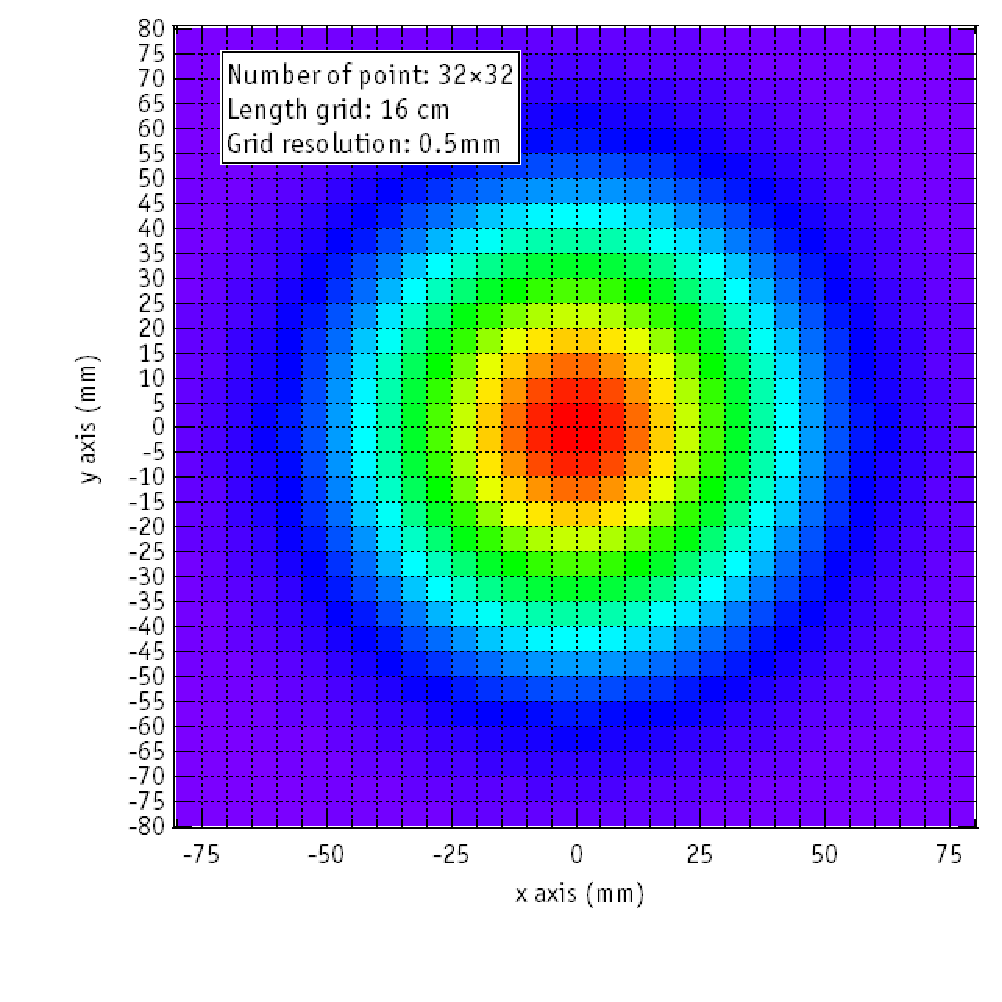
\includegraphics[width = 0.45\textwidth]{T1_FFT1a.pdf}\hfill
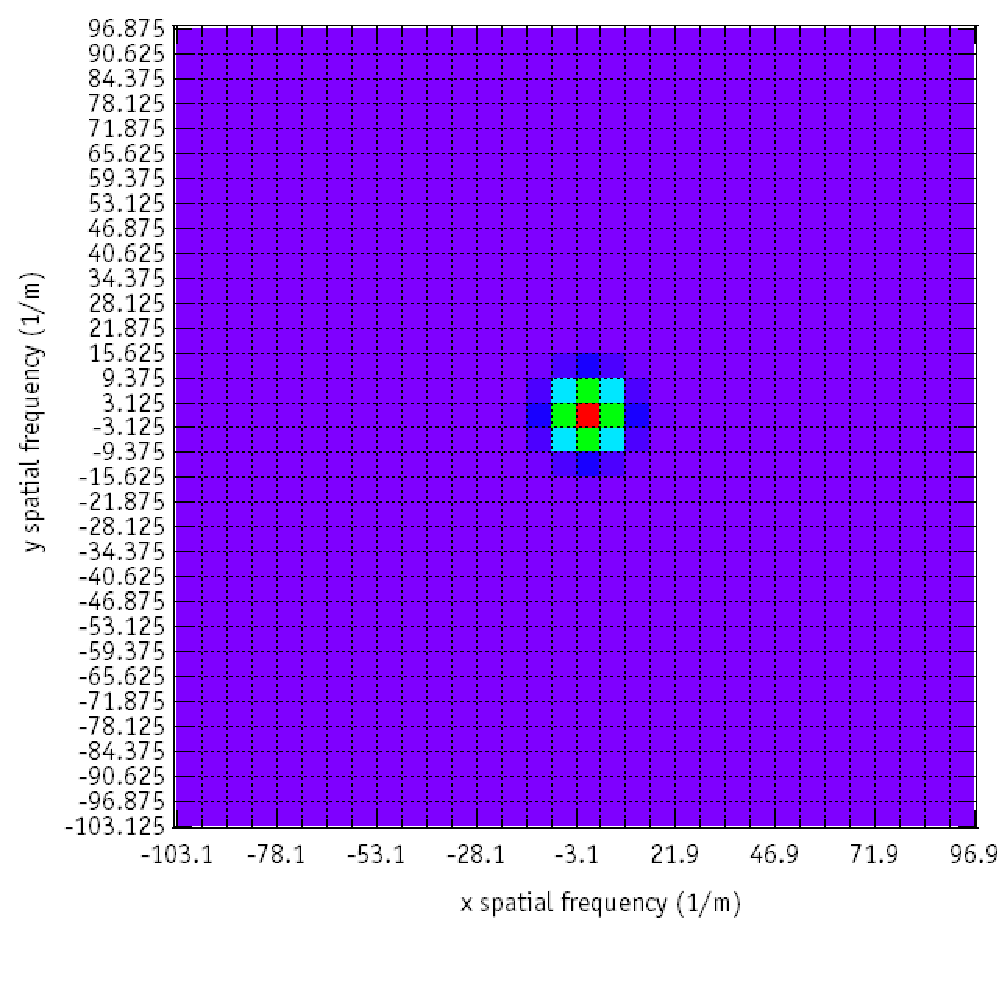
\includegraphics[width = 0.45\textwidth]{T1_FFT1b.pdf}

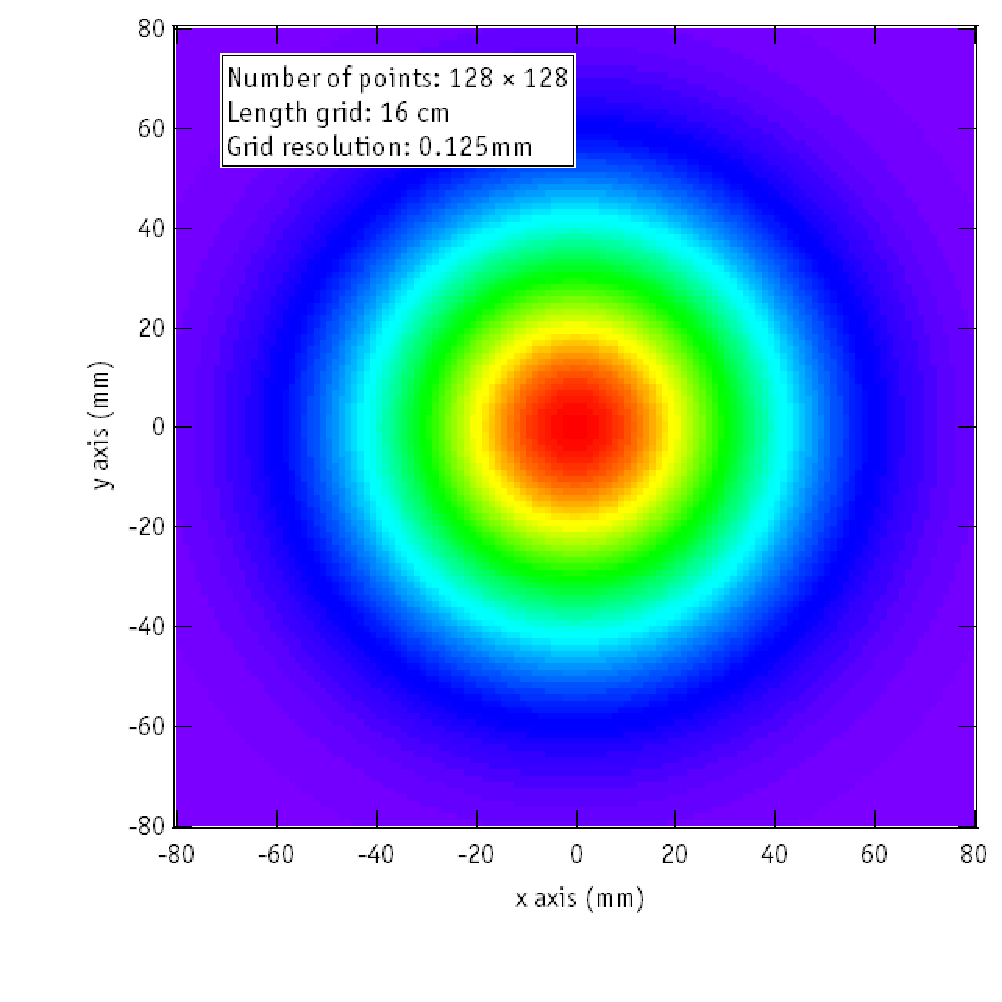
\includegraphics[width = 0.45\textwidth]{T1_FFT2a.pdf}\hfill
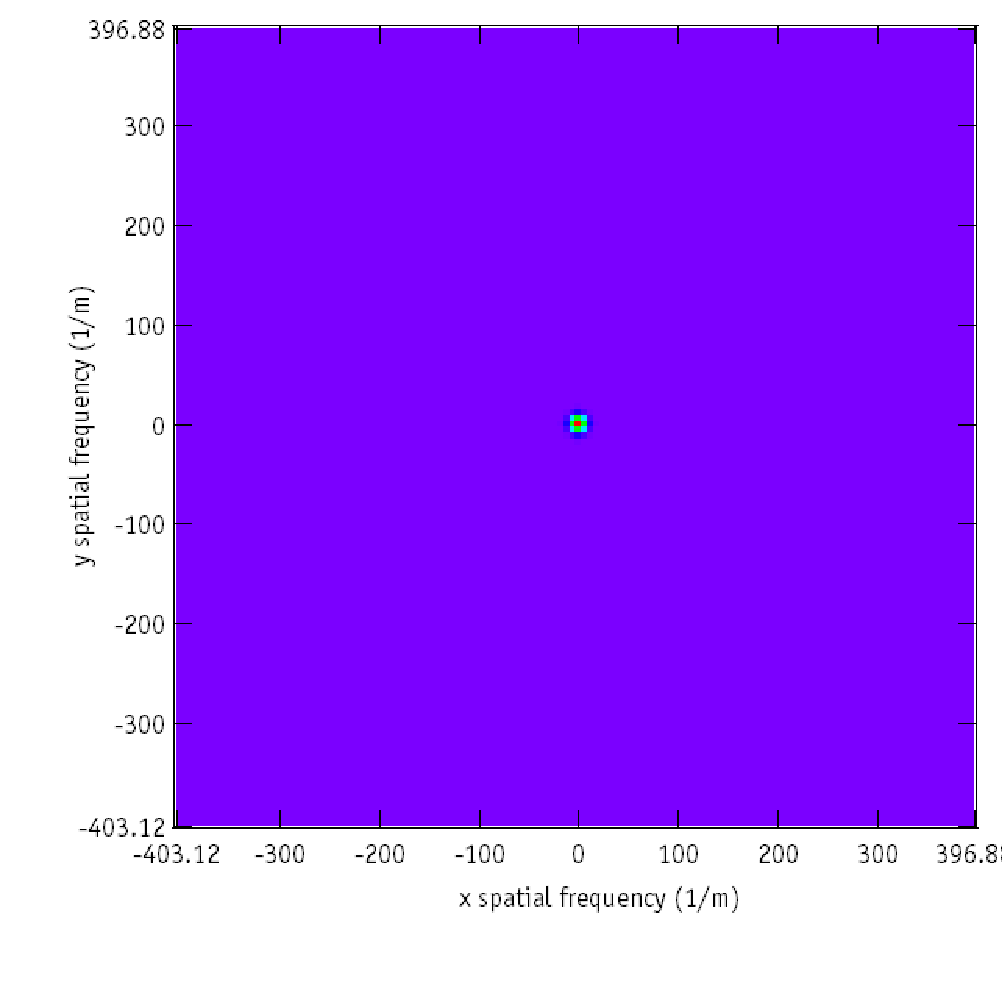
\includegraphics[width = 0.45\textwidth]{T1_FFT2b.pdf}

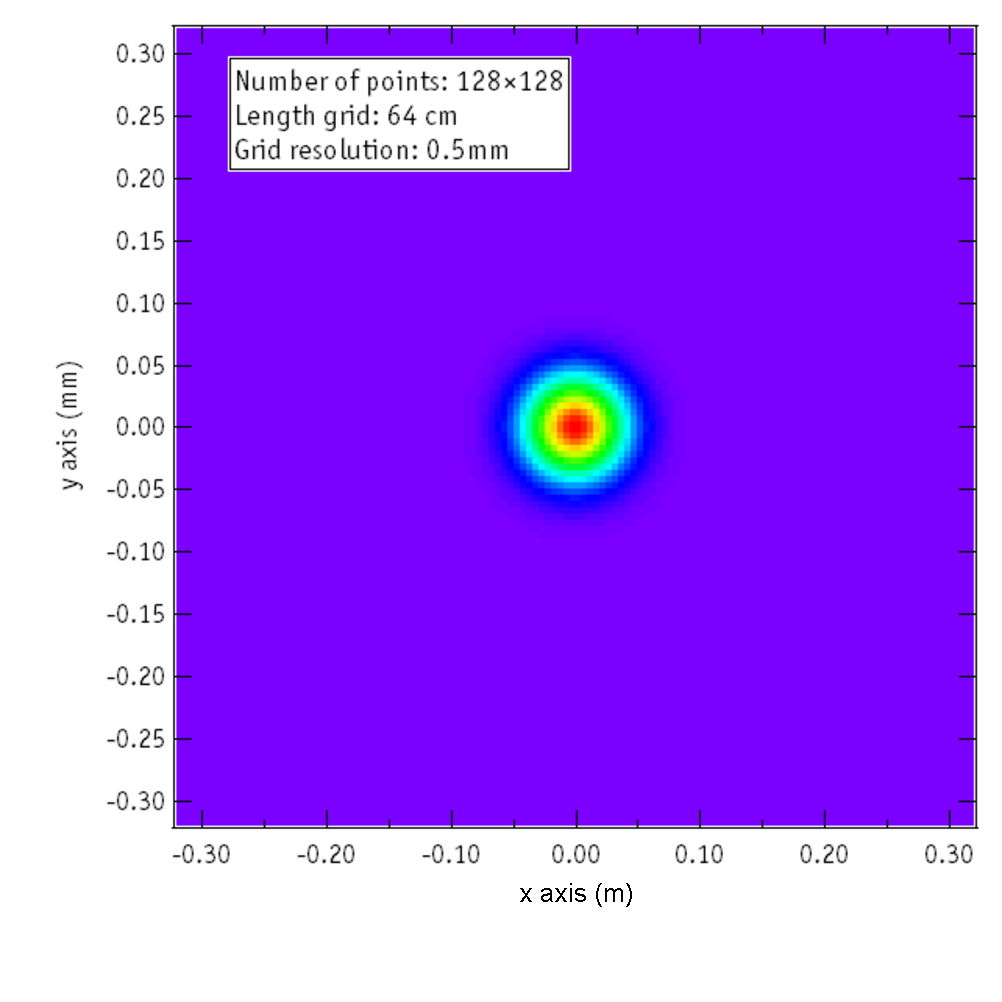
\includegraphics[width = 0.45\textwidth]{T1_FFT3a.pdf}\hfill
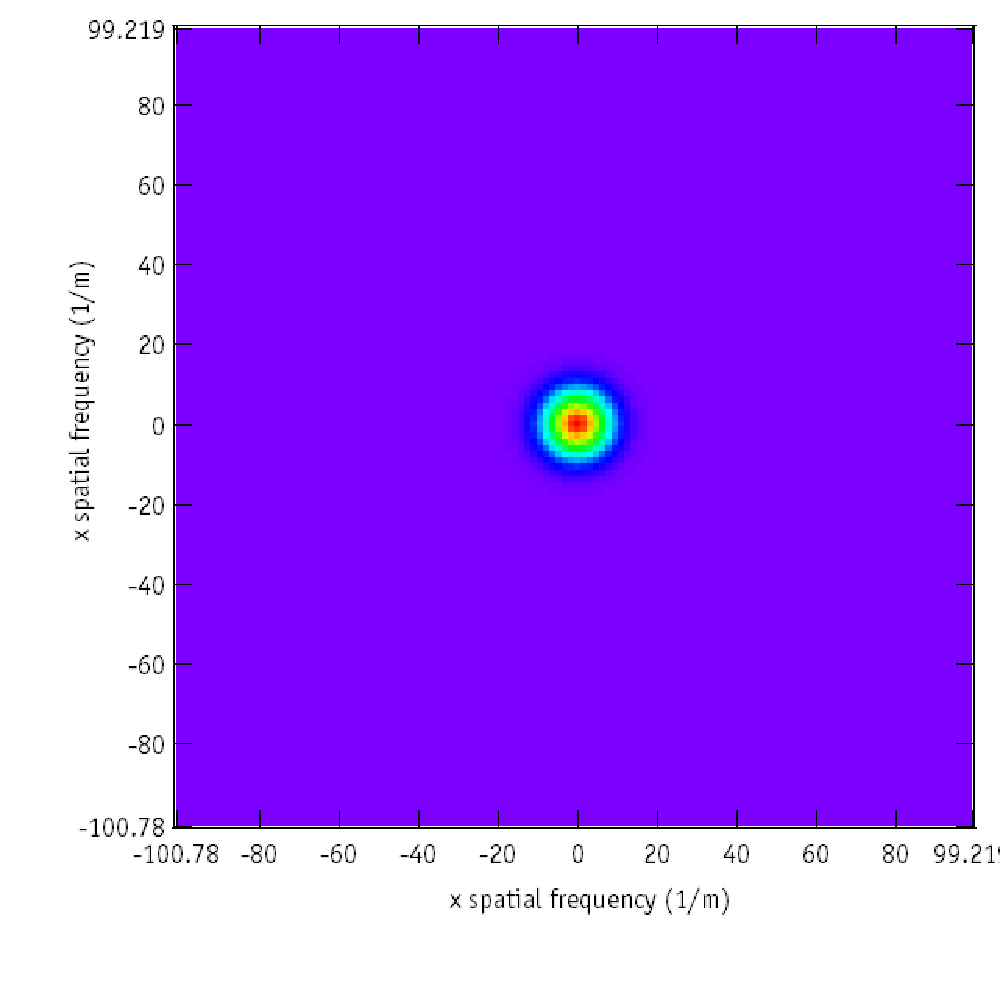
\includegraphics[width = 0.45\textwidth]{T1_FFT3b.pdf}

\end{center}
\vspace*{-0.8cm}
\caption{\label{fig1:FFT} Example of the influence of the physical size of the grid and the number of points used for the representation of a Gaussian beam (left column) and its Fourier transform (right column). As expected intuitively, to have a proper representation of both the Gaussian beam and its Fourier transform it is essential to have simultaneously a large space window (parameter: \textsl{Grid.Length}) and a large number of points (parameter: \textsl{Grid.Num\_point}). For this example the waist of the laser beam is 4~cm. }
\end{figure}

One natural question we could ask is what is the good size of the grid ? The size of the grid must be large enough to represent faithfully the Gaussian beam, no substantial energy from the beam must lay outside the grid. So the dimension of the grid must be \emph{at least} 3-4 times bigger than the biggest beam diameter encountered. A large grid size is also important to sample properly the low special frequency as shown at the bottom of figure \ref{fig1:FFT}. Remarkably even if the laser beam radius increased as the beam propagates from its waist, the amplitude of the Fourier transform is constant along the propagation. Indeed the propagation as shown in equation \ref{eq1:uel11} is simply represented by a phase shift in the Fourier domain.\\

After the physical size of the grid has been chosen, the second important parameter to be decided is the number of points in the grid. Because of the way the discrete Fourier transform is calculated in the FFT algorithm, it is strongly recommended to choose the number of points for the side of the matrix to be a power of 2. Usually a good compromise between speed and accuracy is given for N =64,128 or 256. The influence of the number of points on the accuracy of the results can (and should) always be checked by doing the same simulations with different mesh of the grid.\\

The size of the grid divided by the number of pixels is the dimension represented by one pixel, in other word the resolution of the grid (variable \emph{Grid.step}). Of course, the resolution of the grid must match the size of the physical feature we would like to simulate. For example it is useless to try to simulate the effect of features having a size 1~mm in a mirror map with a grid resolution of 1~cm.\\


We just saw how a square matrix can be used to represent a discrete electric field, so now we can try to simulate its propagation it using the 3 consecutive steps described by equations (\ref{eq1:uel10}), (\ref{eq1:uel11}) and (\ref{eq1:uel12}). During the second step, the Fourier transform of the electric field is multiply by a complex number depending of the distance of propagation and also the spatial frequency. Practically this multiplication is achieved by multiplying pixel by pixel 2 matrices: the Fourier transform matrix with a propagation matrix. The propagation matrix is usually defined before hand and only once since it will be used repeatedly as we will see later in section \ref{sec1.4}. The matlab code at the core of the FFT code is presented in the listing \ref{lis1:start2}, it is the direct sequel from the previous listing where we defined the matrix used to represent the electric field.\\

%\vspace*{1cm}

\begin{lstlisting}[float=tp,caption=The code used to propagate the matrix Field.Start \label{lis1:start2},frame=lines]

% Distance of propagation in meter
Distance_prop = 100;

% Spatial frequency of the pixels in the Fourier space
Grid.axis_fft = -1/(2*Grid.step) + (Grid.vector-1)*1/(Grid.Num_point*Grid.step);

% Define the propagation matrix

Mat_propagation = zeros(Grid.Num_point,Grid.Num_point,'double');

for m = 1:Grid.Num_point
    for n = 1:Grid.Num_point

        Mat_propagation(m,n) = exp(i*(-Laser.k_prop*Distance_prop + ...
            pi*Laser.lambda*(Grid.axis_fft(m)^2 + Grid.axis_fft(n).^2)*Distance_prop));

    end
end

%------------------ Propagate the field ---------------------------

Field.Fourier = fftshift(fft2(Field.Start));       % Do the Fourier transform of the input field
Field.Fourier = Field.Fourier .* Mat_propagation;  % Do the propagation in the frequency domain
Field.End = ifft2(ifftshift(Field.Fourier));       % Do the inverse Fourier transform

% As a result Field.End represents Field.Start propagated over 100 meters
\end{lstlisting}


The propagation of an electric field using a FFT code is an extremely powerful tool. With the FFT code we can propagate any arbitrary profile of the laser beam, not only the beams from the usual Hermite Gaussian set. Such an example is presented in figure \ref{fig4:FFTsquare}. The code used to produce these two plots is given with the OSCAR distribution, the name of the Matlab script is \textcolor{blue}{My\_First\_FFT\_code.m}. The initial field is a theoretical square of uniform amplitude (left plot). The resulting field after the propagation in free space over 100~m is shown in the right plot. A similar result could have been obtained based on the propagation of Hermite Gaussian modes. However to have an accurate representation of the initial field, a very large number of the higher order modes must have been taken into account which requires large amount of computer processing power. The field is discretise on a 1024 $\times$ 1024 matrix. The physical size of the grid is 16~cm $\times$ 16~cm.\\


% 1.5,2,3,0.5
% 14cm 11cm

\begin{figure}
\begin{center}
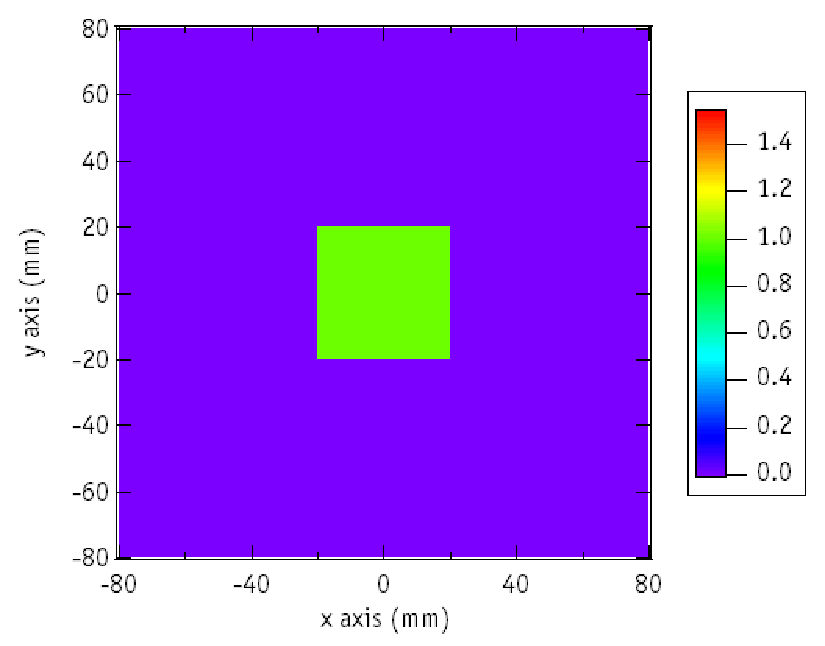
\includegraphics[width = 0.5\textwidth]{T1_Beam_before.pdf}\hfill
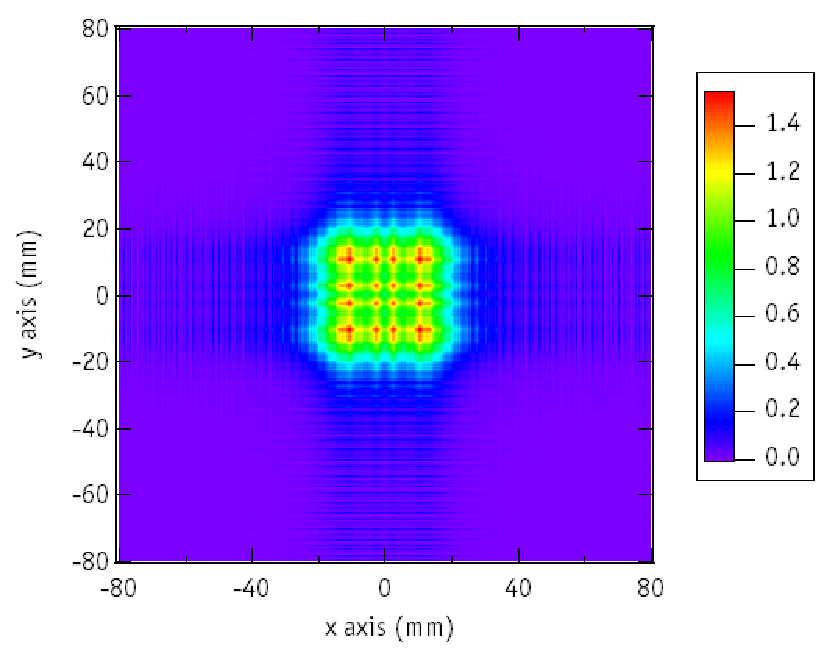
\includegraphics[width = 0.5\textwidth]{T1_Beam_after.pdf}
\end{center}
\caption{\label{fig4:FFTsquare} Propagation of an uniform square of light using our FFT propagation code. The initial square light field is presented on the left plot. The field resulting from the propagation of the initial field over 100~m is shown on the right plot. Structures similar to the Hermitte Gaussian modes begin to emerge when the square field propagates in free space.}
\end{figure}

We arrive now at the end of this section which is dedicated to understand how we can numerically simulate the propagation of an arbitrary laser beam. However having a code only capable to propagate a beam is seldom useful. We are usually more interested to simulate real optical system with mirrors, aperture and imperfect optics. How to include optics in the code is the subject of the next section.\\

\clearpage


\section{Adding realistic optics}
\label{sec1.3}

It is time now to introduce in our simulation two essential optical components: mirrors and lenses. Theses components alter the beam wavefront radius of curvature and so are used for beam shaping (in clear: they make the laser beam smaller or bigger). This can be easily implemented in OSCAR as we will discover in the following paragraphs.



\subsection{Arbitrary wavefront distortion}

Any wavefront distortion can be characterised by its induced optical path length difference $\Delta OPL(x,y)$. In a general manner, when the laser beam crosses a medium of non-uniform refractive index $n(x,y,z)$ the optical path length $OPL(x,y)$ along the optical axis parallel to the 'z' direction can be defined as:

\begin{equation}
OPL(x,y) = \int_0^L n(x,y,z) dz
\end{equation}

With L the length of the medium. Since we are not interested in any constant offset due to the optical path length, it is often more relevant to introduce the optical path length difference $\Delta OPL$ as:

\begin{equation}
\Delta OPL(x,y) = \int_0^L n(x,y,z) dz - \int_0^L n(0,0,z) dz
\end{equation}

The laser field $E_i$ passing trough an element inducing a wavefront distortion characterised by $\Delta OPN(x,y)$ get an additional space dependent phase shift according to:
\begin{equation}
E_o(x,y) = E_i(x,y) \exp{(-j k \Delta OPL(x,y))}
\label{eq1:mir_ref}
\end{equation}

As we can see the effect of the wavefront distortion can be implemented in the physical space and it is not related to any Fourier transform. In fact in any optical FFT code, the Fourier transform is only used to propagate the electric field  over a certain distance. Any other calculations are made in the usual physical space.

\subsection{Mirrors}
\label{sec1:3:2}

One of the most useful wavefront distortion is the one induced by mirrors. A mirror is a reflective spherical surface which is used to steer (flat mirror) or focus the beam (convergent or divergent mirrors). From simple geometrical consideration (see the top left plot in figure \ref{fig4:disct_mirror}) we can calculate the change in sagitta $\Delta s$ as a function of $ \Delta r$ the distance from the mirror center:

\begin{equation}
\Delta s = RofC - \sqrt{RofC^2 - \Delta r^2}
\end{equation}

With $RofC$ the radius of curvature of the mirror. The optical path difference is simply two times the sagitta:

\begin{equation}
\Delta OPL(x,y) = 2\left(RofC - \sqrt{RofC^2 - (x^2+y^2)}\right)
\label{eq1:mir_ref_OPN}
\end{equation}



\begin{figure}
\begin{center}
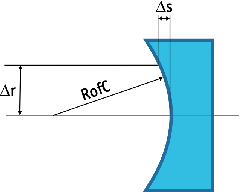
\includegraphics[width = 0.40\textwidth]{Mirrors_scheme1.pdf}\hfill
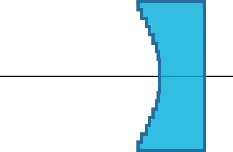
\includegraphics[width = 0.40\textwidth]{Mirrors_scheme2.pdf}\hfill

\vspace*{1cm}

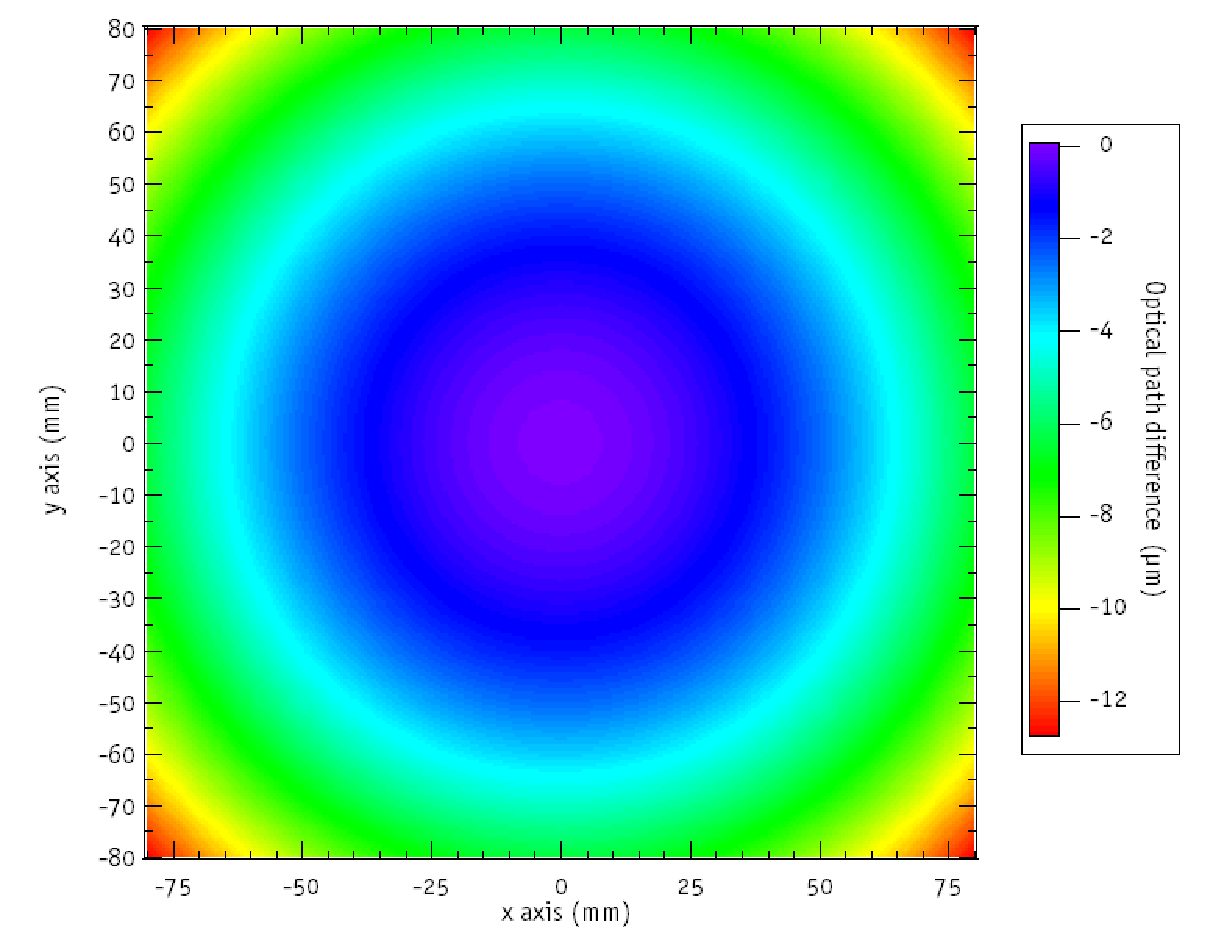
\includegraphics[width = 0.45\textwidth]{Mirror_map_fine.pdf}\hfill
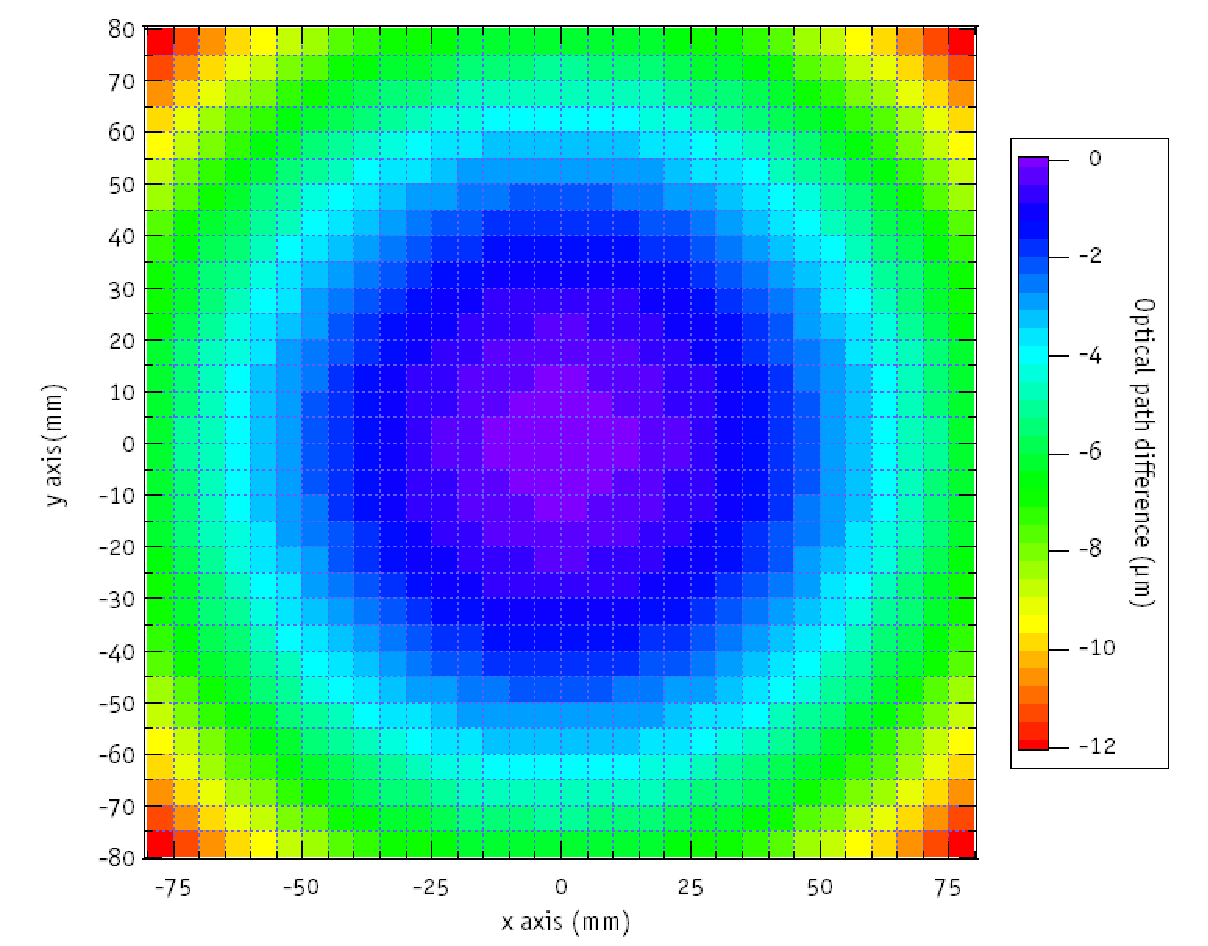
\includegraphics[width = 0.45\textwidth]{Mirror_map.pdf}
\end{center}
\caption{\label{fig4:disct_mirror} Example of the optical path difference induced by 1~km radius of curvature mirror. The optical path difference is simply two times the sagitta of the mirror. The right plot is the left plot discretised on a grid of $32 \times 32$ pixels.}
\end{figure}

Of course since we are using a numerical simulation, the optical path difference representing the mirror has also to be discretized using the same grid as the one used for the laser beam. A discretized optical path difference for a mirror is represented on the right part in the figure \ref{fig4:disct_mirror}.

There is no difficulty to create with Matlab the matrix used to represent the optical path difference induced by a mirror. The value of the optical path as a function of the coordinate $(x,y)$ has previously been shown in equation \ref{eq1:mir_ref_OPN}. The direct Matlab implementation is presented in the listing \ref{lis1:mir1}. By definition in OSCAR a concave mirror has a positive radius of curvature, which means the optical path difference is negative.\\

\begin{lstlisting}[float=htp,caption=The code used to create the mirror matrix \label{lis1:mir1},frame=lines]

% Definition of the mirror radius of curvature in meter
Mirror.RofC = 1000;

% Create mirror grid
Mirror.OPL = zeros(Grid.Num_point,Grid.Num_point,'double');


for m = 1:Grid.Num_point
    for n = 1:Grid.Num_point

        Radius_sqr = (Grid.axis(m)^2+Grid.axis(n)^2);
        Mirror.OPL(m,n) = -2*(Mirror.RofC - sqrt(Mirror.RofC^2 - Radius_sqr));

    end
end
\end{lstlisting}

If the mirror is not perfectly spherical because of thermal lensing effect or because the mirrors are part of a flat beam cavity, we simply have to modify the equation \ref{eq1:mir_ref_OPN} accordingly by adding the known deviation.


\subsection{Lenses}

In OSCAR, we use exactly same procedure as that for mirrors to simulate lenses. The optical path difference induced by the lens is the same as that induced by a mirror whose radius of curvature is two times the focal length of the lens we wish to simulate. The fact that the lens is used in transmission and a mirror in reflection is not relevant in OSCAR. Indeed the evolution of the laser beam confined between two mirrors can always be simulated by the propagation of a laser beam passing through a periodic system of lenses\cite{Kogelnik}.


\subsection{Aperture}

\label{sec1:aperture}

Apertures can be represented by two complementary physical areas: one area transmits integrally the light falling on it whereas the other area blocks integrally the light. Apertures are useful to simulate correctly finite size optics. In OSCAR, the optical path difference representing a mirror is defined over the whole calculation grid independently of the real size of the mirror. To simulate a finite size mirror, we multiply the reflected field by an aperture which has the same diameter as that of the mirror. The aperture simulates the fact that any light falling outside the mirror is lost.\\

Practically, an aperture $A(x,y)$ is represented by matrix of $0$ and $1$. A $0$ at the position $(x,y)$ indicates that the light is blocked and a $1$ indicates that the light is transmitted. An example of a circular aperture is presented in figure \ref{fig1:aperture}. So to simulate the reflection from a finite size mirror, we can include the aperture effect in the previous equation \ref{eq1:mir_ref}:

\begin{equation}
E_o(x,y) = E_i(x,y) \exp{(-j k \Delta OPL(x,y))} A(x,y)
\end{equation}


% 1.5,1.5,3,0.5

\begin{figure}
\begin{center}
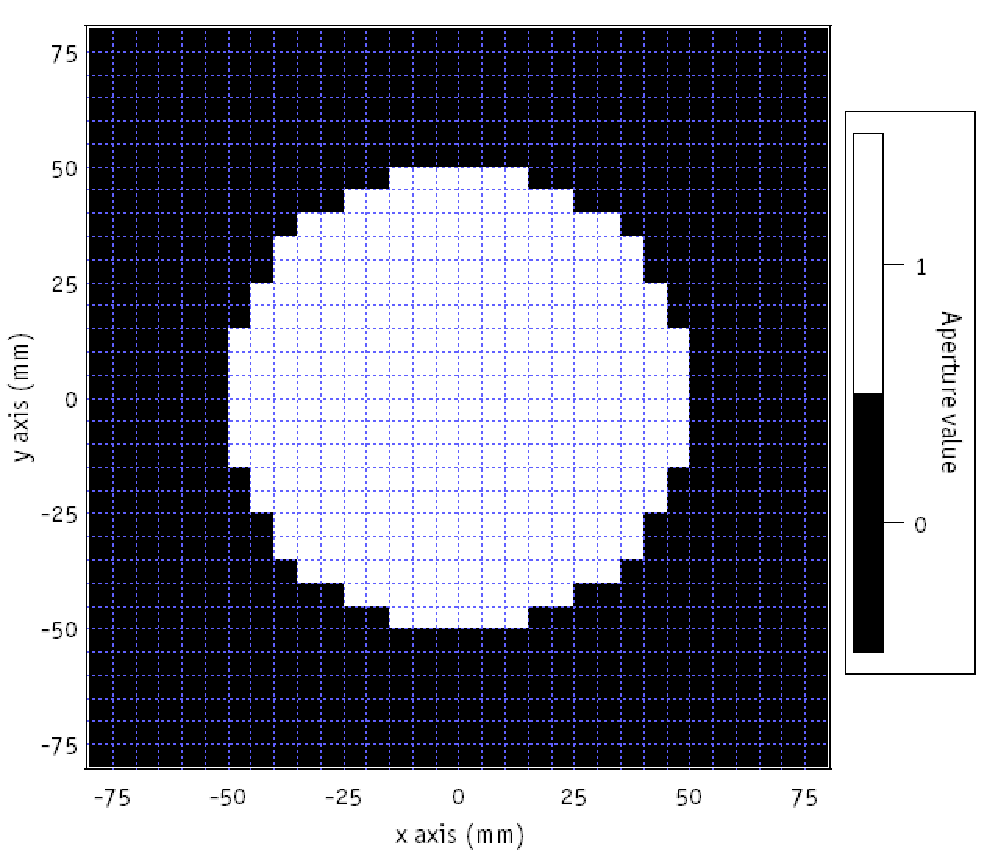
\includegraphics[width = 0.8\textwidth]{Mirror_mask.pdf}
\end{center}
\caption{\label{fig1:aperture} Plot of the 2D matrix representing a circular aperture of diameter 10~cm. The number of points for the grid is $32 \times 32$ points and the physical size of the grid is 16~cm $\times$ 16~cm.}
\end{figure}

As for the optical path induced by the mirror, we can also define a matrix representing the aperture. In the OSCAR code this matrix is called $Mirror.mask$. This matrix is only filled with $0$ and $1$, $1$ when the pixel is inside the mirror and $0$ otherwise. The simple Matlab code to create a circular aperture in OSCAR is described in the listing \ref{lis1:aper1}.\\

\begin{lstlisting}[float=htp,caption=The code used to create a circular aperture \label{lis1:aper1},frame=lines]

% Define aperture diameter in meter
Aperture_diameter = 0.1;

Mirror.mask = zeros(Grid.Num_point,Grid.Num_point,'double');

for m = 1:Grid.Num_point
    for n = 1:Grid.Num_point

        Radius = sqrt(Grid.axis(m)^2+Grid.axis(n)^2);
        if (Radius < Aperture_diameter/2)
            Mirror.mask(m,n) = 1;
        end
    end
end

\end{lstlisting}

\subsection{Code implementation}
\label{sec1:3:5}
To simulate the reflection of an electric field by a mirror (or a transmission through a lens), we define a function called \emph{Propa\_mirror}. The function takes for parameters the input electric field, the optical path difference induced by the mirror and the reflectivity of the mirror as shown in the listing \ref{lis1:refl1} . The output of the function is the electric field after the reflection on the mirror. The function is a direct implementation of the equation \ref{eq1:mir_ref}.

The aperture of the mirror is also included in the reflection however it is not an argument of the function \emph{Propa\_mirror} since we suppose that the mirrors have all the same diameter, so the aperture matrix is constant\footnote{The function can easily be modified if the mirrors have different sizes}. in the function, the reflectivity of the mirror is scalar, which means the reflectivity is homogenous and constant over the mirror surface. The reflectivity of the mirror can also be defined as a matrix if the reflective coating is not perfectly uniform.

\begin{lstlisting}[float=htp,caption=The function used to simulate the reflection of an electric field by a mirror\label{lis1:refl1},frame=lines]

function Output = Propa_mirror(Wave_field, Wave_mirror, reflectivity)

global Mirror;
global Laser;

Output = Wave_field .* exp(i * Wave_mirror*Laser.k_prop) * reflectivity .* Mirror.mask;

\end{lstlisting}


\section{Simulating a Fabry Perot cavity}
\label{sec1.4}

Since we have seen in the two last sections how to propagate a laser beam in free space (section \ref{sec1.2}) and how to simulate the reflection by a mirror (section \ref{sec1.3}), we have all what we need to simulate a Fabry Perot cavity.

A Fabry Perot cavity is usually constituted by two mirrors facing each other. Between these two mirrors, a light field is circulating, bouncing back and forth between the two reflective coatings. One of the main interest of the Fabry Perot is that the optical power of the circulating field can be much higher than the power of the input field. With OSCAR, it is possible for a given input field to calculate the total circulating power, reflected power and transmitted power as well as the spatial profile of all the light fields.\\

The method used by OSCAR to calculate the circulating field in a Fabry Perot cavity is well known for most readers. Indeed, the same method is often used in undergraduate lectures to calculate analytically the circulating field in the cavity\cite{Cav_circ}. OSCAR calculates the circulating field by propagating back and forth the laser beam between the two mirrors and then summing all the fields at one particular plane as shown in figure \ref{fig1:cavity}.

\begin{figure}
\begin{center}
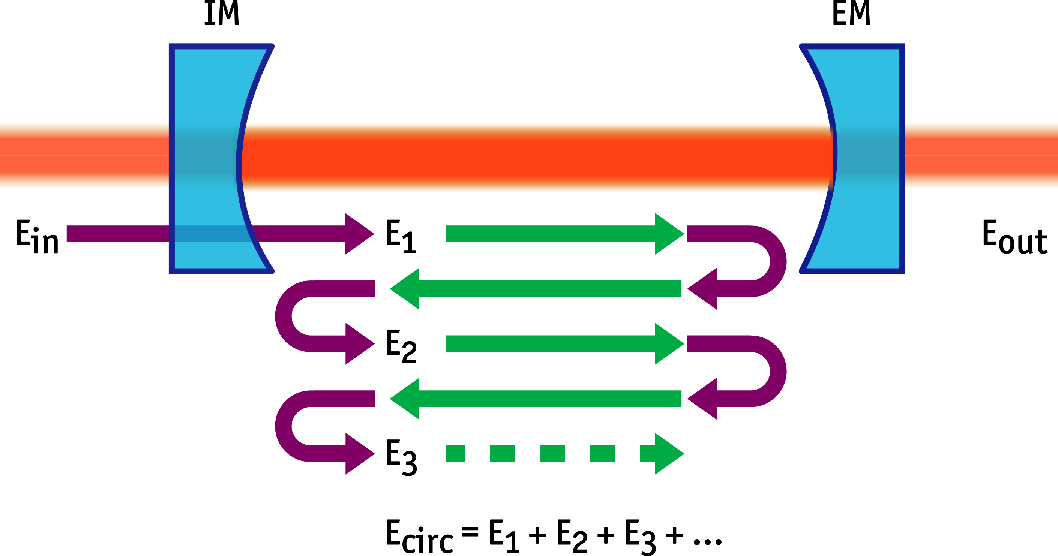
\includegraphics[width = 0.95\textwidth]{C1_cavity.pdf}
\end{center}
\caption{\label{fig1:cavity} Description of the algorithm used in OSCAR to calculate the circulating field in a Fabry Perot cavity. The violet arrows represent a change in phase for the light field which is described by equation \ref{eq1:mir_ref} and the green arrows represent the propagation of the light field using a FFT code. From $E_i$ to $E_{i+1}$, the light field has undergone one round trip in the cavity. IM and EM stand respectively for Input Mirror and End Mirror.}
\end{figure}

In more details, we can write the OSCAR algorithm used to compute the circulating power. Using the notation from the figure \ref{fig1:cavity} the different consecutive steps can be described as:

\begin{enumerate}
  \item Define the cavity parameters as well as the mirror profiles and the input beam.
  \item Propagate the input beam $E_{in}$ through the input mirror . For this purpose the input mirror can assimilated to a lens, so the listing \ref{lis1:refl1} can be used. As a result, we obtain the field $E_1$.
  \item After one round trip in the cavity, the field $E_1$ becomes $E_2$. One round trip in the cavity consists specifically of one propagation through the cavity length using the FFT code, one reflection on the end mirror, another propagation back to the input mirror and then finally a reflection on the input mirror.
  \item Repeat the last operation to create the set of electric field $E_i$.
  \item Then sum all the field $E_i$ to have the cavity circulating power $E_{circ}$. The number of light field $E_i$ to be considered to have an accurate result depends on the finesse of the cavity.
  \item The transmitted field $E_{out}$ is simply the circulating field transmitted through the ETM.
\end{enumerate}

In this above pseudo-code, we did not mention any resonance condition to maximise the circulating power in the cavity. Practically, we should always define the round trip phase shift for the field in the cavity (or a microscopic position shift for the cavity length) before calculating the cavity circulating power. The round trip phase shift allows us to set the cavity to be resonant for the fundamental mode or any other optical modes if necessary. The procedure to find the suitable resonance length is detailed in the next chapter in section \ref{sec2.2}.

\section{Further reading}

In this chapter, only a general and simplistic view of the FFT code has been presented. To have a better understanding of the power and limit of the code some further reading is highly recommended. Here some suggestions:
\begin{itemize}
  \item The thesis from Brett Bochner\cite{Bochner} which programmed one of the first FFT code used by LIGO is a mine of treasures. The chapter two of this thesis about the technical realization of an optical FFT code contains some essential issues to grasp for a successful code, for example how the radius of curvature of the mirror can set an upper limit on the resolution of the grid, the use of aliasing filters or methods to calculate the steady state fields.

  \item Andrew Trigdell wrote also a FFT code in the ANU group. His master thesis may be hard to find but a following article\cite{Tridgell} gives some good insights of the procedures involved in the code.

  \item A wonderful article to understand how to create a simple and robust FFT code to simulate high finesse cavity has been written by Partha Saha. The explanation how to calculate the steady state cavity circulating field is crystal clear and very elegant (however the end of the article may appear a little bit more obscure at the first reading).

  \item Technics to build a FFT code (and some other optical numerical codes) can be found in the recent thesis of Juri Agresti\cite{Juri}. This thesis is also an excellent example about how to deal with non spherical mirror.

 \item One of the first article describing how to use a FFT to calculate the eigen modes of a cavity by Gordon and Li\cite{Gordon}. Although the article is 40 years old, all the modern FFT program are still based on the fundamental method explained in this paper.

\end{itemize}









\part{OSCAR V1: the classic version}

\chapter{The OSCAR code in details}
\label{chap2}

This chapter is a step by step guide to run OSCAR \textbf{prior to version 3}. Using the simple example of a Fabry Perot cavity, we will describe the essential procedures and give some hints in order to obtain valid results. The different scripts for this example can be found in the folder entitled \textcolor{blue}{Calculate\_Pcirc}. To run the full simulation, execute the Matlab script called \textcolor{blue}{Run\_OSCAR.m}.\\

To be able to run all the examples quoted in this chapter, an older version of OSCAR must be used: the version 1. This chapter is still there for legacy reason since all the principles described are the base for the current version 3.

%\emph{For version 3.21 and above, the example scripts are now in the folder \textcolor{blue}{Examples}. To calculate the circulating field in a cavity please use the script called \textcolor{blue}{Example\_Pcirc.m}.}

\section{The cavity to simulate}
\label{chap2:1}
We are interested to simulate a Fabry Perot cavity with a slightly mismatched input beam. The physical parameters of the optical system to simulate are summarized in table \ref{tab2:param}. After defining our cavity, we have to choose 2 essential parameters for our simulation: the physical size of the grid \textsl{Grid.Length} and the number of points of the grid \textsl{Grid.Num\_point}. Our grid must include the mirror aperture, so the size of the grid must be at least equal to the mirror diameter. In our case the mirrors have a diameter of 25~cm, so the dimension of the grid could be 30~cm $\times$ 30 cm. Then, we can think about the number points required to sample the laser beam. Of course, a large number of points leads to accurate results but at the price of a lengthy computational time. From experience a grid with 128 $\times$ 128 is a safe choice to simulate a cavity with smooth mirrors.

\begin{table}[tbp]
  \centering
  \caption{\label{tab2:param} Parameters of the input beam and the Fabry Perot cavity we wish to simulate. The variable name is the name of the variable in the OSCAR program and so also in the Matlab workspace.}
\begin{tabular}{|l r|>{\slshape}l|c|}
  \hline
  {\large\strut} Parameters & & Variable name & Value \\
  \hline
  {\large\strut} Cavity length &(m) & Length\_cav & 1000 \\
  {\large\strut} Substrate refractive index & & Refrac\_index & 1.5 \\
  {\large\strut} Mirror diameter &(mm) & Mirror.Diam & 250 \\
  \hline
  \hline
  \multicolumn{2}{|c|}{{\large\strut} \textbf{Input laser}} \\
  \hline
  {\large\strut} Wavelength &(nm) & Laser.lambda & 1064 \\
  {\large\strut} Beam radius &(mm) & Laser.size & 20 \\
  {\large\strut} Wavefront curvature &(m) & Laser.radius & -2000 \\
  {\large\strut} Optical power &(W) & Laser.power & 1 \\
  \hline
  \hline
  \multicolumn{2}{|c|}{{\large\strut} \textbf{Input mirror}} \\
  \hline
  {\large\strut} Radius of curvature &(m) & ITM.RofC & 2500 \\
  {\large\strut} Transmission & & ITM.T & 0.005 \\
  {\large\strut} Loss &(ppm) & ITM.L & 50 \\
  {\large\strut} Reflectivity & & ITM.R & 1 - (Transmission + Loss) \\
  \hline
  \hline
  \multicolumn{2}{|c|}{{\large\strut} \textbf{End mirror}} \\
  \hline
  {\large\strut} Radius of curvature &(m) & ETM.RofC & 2500 \\
  {\large\strut} Transmission &(ppm) & ETM.T & 50 \\
  {\large\strut} Loss &(ppm) & ETM.L & 50 \\
  {\large\strut} Reflectivity & & ITM.R & 1 - (Transmission + Loss) \\
  \hline
\end{tabular}
\end{table}

To fasten the calculations, we suppose the substrate of the input and end mirror to be thin, so the substrates are equivalent to thin lenses for a beam passing through. We also suppose the laser beam to be defined at the input mirror reflective coating but still outside the cavity, so we do not have to propagate the input laser beam in space or in the substrate before the transmission through the input mirror.

\section{Declaration and initialisation}
\label{sec2:2.2}
The first Matlab script to run when starting a simulation is the script called \textcolor{blue}{CreateField.m}. During this script all the variables required for the simulation will be defined. That includes as well the matrix representing all the mirror maps (in reflection and transmission), mirror aperture(s) and the matrix describing the input laser beam. For coherence, all the variables must be defined in the International System of Units (SI), which means all the variables representing a length are in meter.

The script \textcolor{blue}{CreateField.m} is most of the time self explaining and does not require extensive thinking. First the variables \textsl{Grid.Length} and \textsl{Grid.Num\_point} are defined and then all the variables listed in the table \ref{tab2:param} are given. From the given parameters, the mirror aperture matrix is created (according to the listing \ref{lis1:aper1}), following by the propagation matrix (listing \ref{lis1:start2}), the mirror $\Delta OPL(x,y)$ maps (listing \ref{lis1:mir1}) and finally the matrix of the input beam.

For convenience, two matrices extensively used in intermediate calculations are also defined: \textsl{Grid.D2} is a matrix where the value of each pixel is the distance between the pixel and the origin, i.e $value = \sqrt{x^2+y^2}$ and \textsl{Grid.D2\_square} is the previous matrix but with every pixel squared, i.e $Grid.D2\_square = Grid.D2.^2$

\section{Finding the resonance length}
\label{sec2.2}

In this section the role of one of the most important script in OSCAR is explained. This script is called \textcolor{blue}{Find\_resonance\_length.m} and is used to find the microscopic shift of the cavity length which is required to be on resonance. This script is essential because before calculating the circulating field in a Fabry Perot cavity, the cavity has to be set on resonance where the circulating power of the fundamental mode TEM$_{00}$ will be maximized. In the domain of gravitational wave detection, all the optical cavities of the detector are resonant for the fundamental mode or very near the resonance as in the case of DC-readout or detuned signal recycling.\\


\subsection{Setting the resonance the length}

The first thing to understand is how OSCAR implements a microscopic length shift of the cavity length. For example, for setting the cavity on resonance we have to shift the cavity length (called \textsl{Length\_cav}) by a value $\delta L$ with $\delta L$ smaller than half a wavelength. The first (and the simplest) idea is to the set a new cavity length to \textsl{Length\_cav}$ + \delta L$. This solution is perfectly viable and gives correct result in Matlab for kilometer long cavities. However, from a numerical point of view it may not be the most robust solution since we have to add a length of the order of the kilometer with a length smaller than one micrometer\footnote{For reference, in Matlab the relative accuracy in the number representation can determined with the function eps('double'), on my computer it is of the order $10^{-16}$.}.

Another solution to set the cavity on resonance, is to add after each light round trip in the cavity a constant phase shift. This is this solution that we use in OSCAR. So to simulate a cavity length shift of $\delta L$, a phase shift of $ k 2 \delta l$ is added after each round trip of the field $E_i$. Practically, when calculating the circulating field, the matrix of the field $E_i$ is multiplied by a scalar factor $\exp{(j k 2 \delta l)}$ just before the field is reaching back the input mirror. To be consistent with the previous chapter it must have been $\exp{(-j k 2 \delta l)}$ however in the OSCAR code, it is implemented as $\exp{(j k 2 \delta l)}$, the sign convention can be arbitrary (as soon as it is kept constant for all the procedures).

In OSCAR, the variable which represents the shift in the cavity length necessary to be on the desired resonance is called \textsl{Length.reso\_zoom}. To determine the right value for \textsl{Length.reso\_zoom}, the script \textcolor{blue}{Find\_resonance\_length.m} has to be run first. By convention, \textsl{Length.reso\_zoom} is in fact $\delta l/2$ which means that the variable \textsl{Length.reso\_zoom} represents the shift in the round trip length to make the cavity resonant. With this convention if \textsl{Length.reso\_zoom} is shifted by one wavelength, the resonance frequency is shifted by one free spectral range.\\


\subsection{Finding the resonance the length in details}
\label{sec2:3}
The principle to find the resonance length of the cavity is quite simple: the cavity circulating power is monitored as the cavity round trip length is scanned over one wavelength. The resonance length \textsl{Length.reso\_zoom} is the length which maximises the circulating power. A typical plot of the circulating power as a function of the microscopic cavity round trip length is shown in figure \ref{fig2:cavres}.

The first idea to draw a plot of the cavity circulating power as a function of the cavity tuning is straight forward. We simply run the FFT code to calculate the circulating power for all the different detuning we would like to test. For example, in figure \ref{fig2:cavres}, the horizontal axis which spans over one wavelength is divided into 2000 points. So we can imagine to run the FFT code, 2000 times for each particular round trip length. This procedure is absolutely correct, however extremely slow.

% 23 12

\begin{figure}
\begin{center}
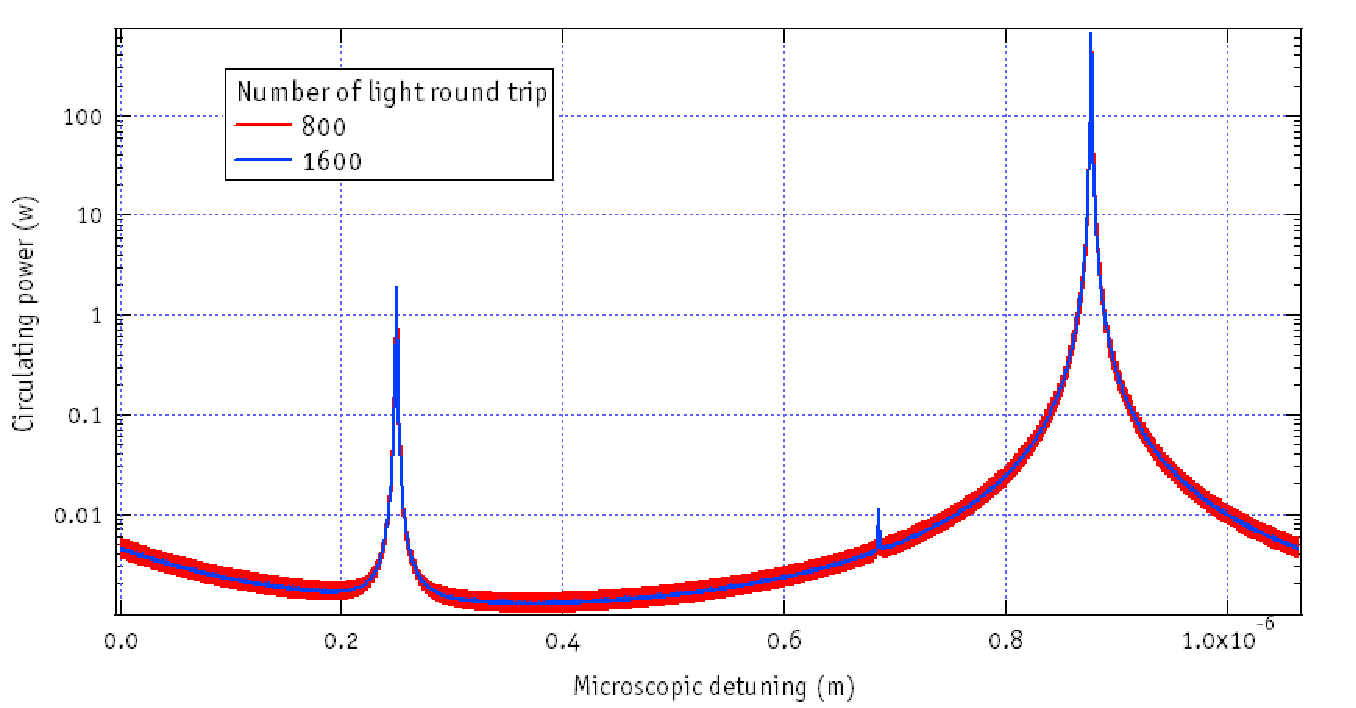
\includegraphics[width = 0.95\textwidth]{Fig2_resonance.pdf}
\end{center}
\caption{\label{fig2:cavres} Circulating power in the cavity as the function of the macroscopic round trip length detuning scanned over one wavelength. The higher peak indicates the resonance position of the fundamental mode TEM$_{00}$. We can also notice two smaller peak revealing the presence of higher order optical modes, this is a strong proof that the input beam is not matched with the cavity eigen mode. The figure has been plotted for two values of \emph{Length.nb\_iter}, this variable determines the number of field $E_i$ to cumulate when calculating the circulating power. On resonance, the build up circulating power is of course higher when we use 1600 fields instead of 800 (even if it is not obvious in the figure due to the large vertical scale).}
\end{figure}



Practically, in OSCAR to draw the plot in figure \ref{fig2:cavres}, a technique first described by Gordon and Li\cite{Gordon} is employed. The principle is explained by the follow step:
\begin{enumerate}
  \item First all the fields $E_i$ are calculated and stored for an arbitrary position of the cavity tuning (so for an arbitrary resonance length). This step is only done once.
  \item The circulating field $E_{circ}$ for a particular microscopic round trip length $\delta l$ is built up by summing all the field $E_i$ with the proper phase shift:
      \begin{equation}
      \label{eq2:buildup}
      E_{circ} = \sum_i E_i \exp\left(j k \delta l \right)
      \end{equation}
  \item Repeat the previous step over all the detuning length $\delta l$ we wish to try.
\end{enumerate}

The advantage of this technique is that the FFT code is just called once to calculate the field $E_i$, then the reconstruction of the power buildup for the various length detuning is just a matter of summing and multiplication. The only limitation of this technique is that a huge amount of memory is required since all the fields $E_i$ are to be stored. For example if we would like to store 500 complex matrices of 256 $\times$ 256 points,  500 megabytes of free memory is required.

%Example iter_propafield

\subsection{Code implementation}
\label{sec2:2.2.3}
To calculate the resonance length in OSCAR, so to calculate the value of \textsl{Length.reso\_zoom}, several script are involved. Here the list:

\begin{itemize}
  \item \textcolor{blue}{Find\_resonance\_length.m} is the main procedure. At the end of the procedure, the variable \textsl{Length.reso\_zoom} which maximises the cavity circulating power, is returned. This script is divided into two similar parts: first part the cavity detuning is scanned over one wavelength, then in the second part we scan around the maximum position found after the first scan with a much greater detuning resolution (we zoom around the maxima found in the first part). At the beginning of the script, two important variables are defined: \emph{Length.nb\_iter} determines the number of step used to scan the cavity over one wavelength (usually 2000) and \emph{Length.nb\_propa\_field} is the number of light round trip taken into account when calculating the circulating power (i.e. number of fields $E_i$ we used).
  \item \textcolor{blue}{Propagate\_Field.m} is script called at the beginning of \textcolor{blue}{Find\_resonance\_length.m}. This script calculates all the intermediate field $E_i$ using the FFT code and stores the results in one variable called \emph{Field.propa}. \emph{Field.propa} is a 3D matrix having with a size of \emph{Grid.Num\_point} $\times$ \emph{Grid.Num\_point} $\times$ \emph{Length.nb\_propa\_field}.
  \item \textcolor{blue}{Build\_Field\_Cavity.m} is a function called intensively by \textcolor{blue}{Find\_resonance\_length.m}. This function takes for argument a length detuning and returns the build-up circulating  field following the equation \ref{eq2:buildup}.
  \item \textcolor{blue}{Calculate\_power.m} is a simple function which takes for input a 2D electric field and returns the optical power in Watt of the input field.
\end{itemize}

\subsection{Some comments}

The method used by OSCAR to find the resonance length is slow. In term of calculation time, it is the bottleneck of this FFT code. It is possible to find different approaches to calculate the resonance length and some are much faster, however I prefer to keep the method described above. Why ? because the plot of the circulating power as a function of the wavelength (figure \ref{fig2:cavres}) contains numerous essential information which help debugging the simulation or understanding the optical system. Here some examples:

\begin{itemize}
  \item If during a simulation, the plot of the circulating power as a function of the detuning does not look like the one in figure \ref{fig2:cavres}, but instead looks flat or with very small bumps it means the cavity is unstable. In the same idea, the linewidth of the peak in the plot is inversely proportional to the finesse of the cavity so it is a good indication of the round trip loss in the cavity.
  \item The number of peaks in the plot is directly proportional to the mode mismatching or misalignment between the input beam and the cavity eigen modes. In the case of perfect mode matching only one peak is present, which means that all the input light coupled to only one optical mode (preferably the fundamental Gaussian beam). By looking at the shape of the higher order modes which are excited (see figure \ref{fig2:cavres}), we could have an idea of the type of mode mismatching and/or misalignment. For example, if all the higher order modes which are excited looks like TEM$_{m0}$, it means the input beam is misaligned with the cavity axis in the horizontal direction.
  \item Finally, since we also know the position detuning for the higher order modes, we can also set the cavity on the resonance of the higher order modes if necessary. The knowledge of the relative detuning position of the resonance for the higher order modes allows also the calculation of the Gouy phase shift between higher order modes (which maybe unknown if the beam is not Gaussian).\\
\end{itemize}

We do not need a lot of light round trip to have an accurate result for the resonance length position. In the previous example, we use 800 or 1600 round trips for the calculation but only 50 round trips can already give a correct answer. The only difference is that the plot of the circulating power as a function of the detuning may not look so sharp (so we can miss the presence of smaller resonance peaks).\\

For verification purpose, it may be important to check the shape of the circulating field for different detuning length. For example to display the circulating field for a detuning position of $2.5 \times 10^{-7}$ which corresponds to the first left peak in the figure \ref{fig2:cavres}, we just have to write the following command in Matlab:

\vspace*{0.5cm}

$>>$ Plot\_Field(Build\_Field\_Cavity(2.5E-7))

\vspace*{0.5cm}
\noindent With such command, we can check which optical modes can build up in the cavity. The 2D amplitude of the three optical modes corresponding to the three peaks in figure \ref{fig2:cavres} are presented in figure \ref{fig2:HOM} in the order of increasing detuning.

% 17 14

\begin{figure}
\begin{center}
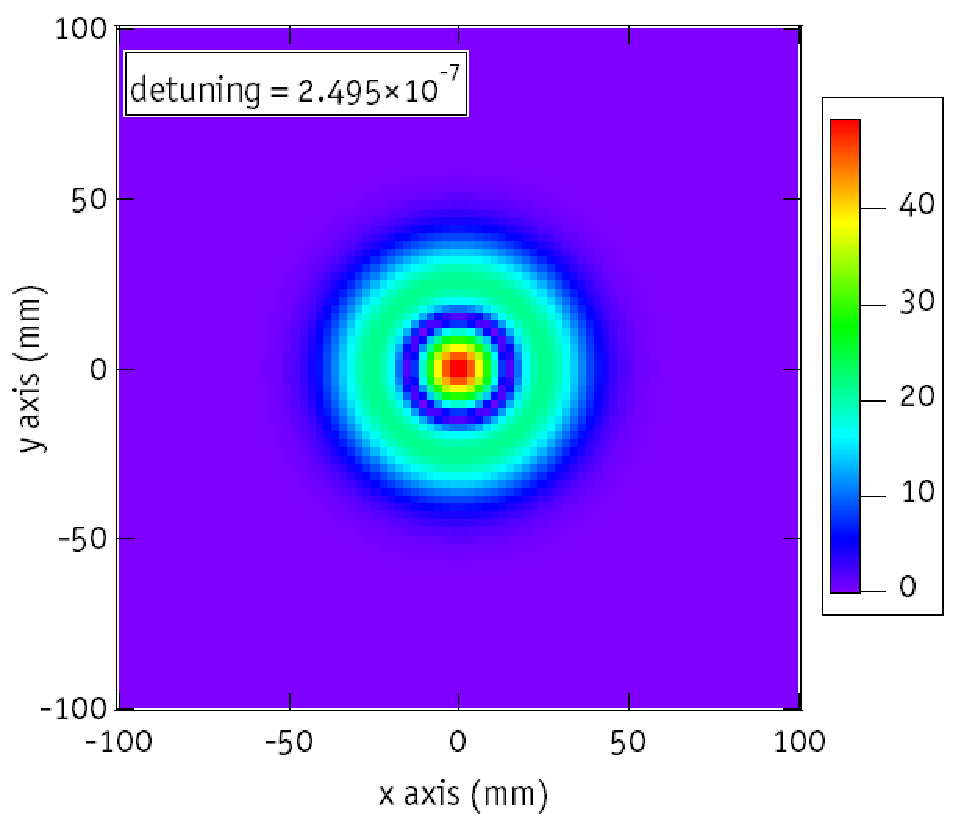
\includegraphics[width = 0.33\textwidth]{Fig2_mode1.pdf}\hfill
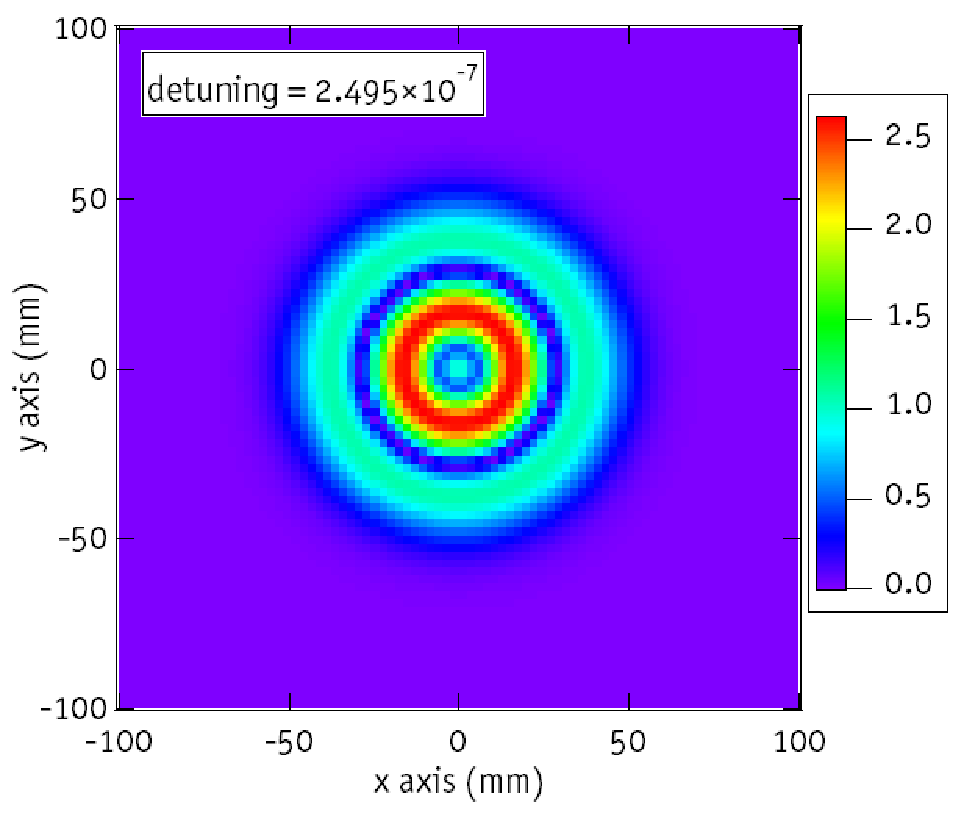
\includegraphics[width = 0.33\textwidth]{Fig2_mode2.pdf}\hfill
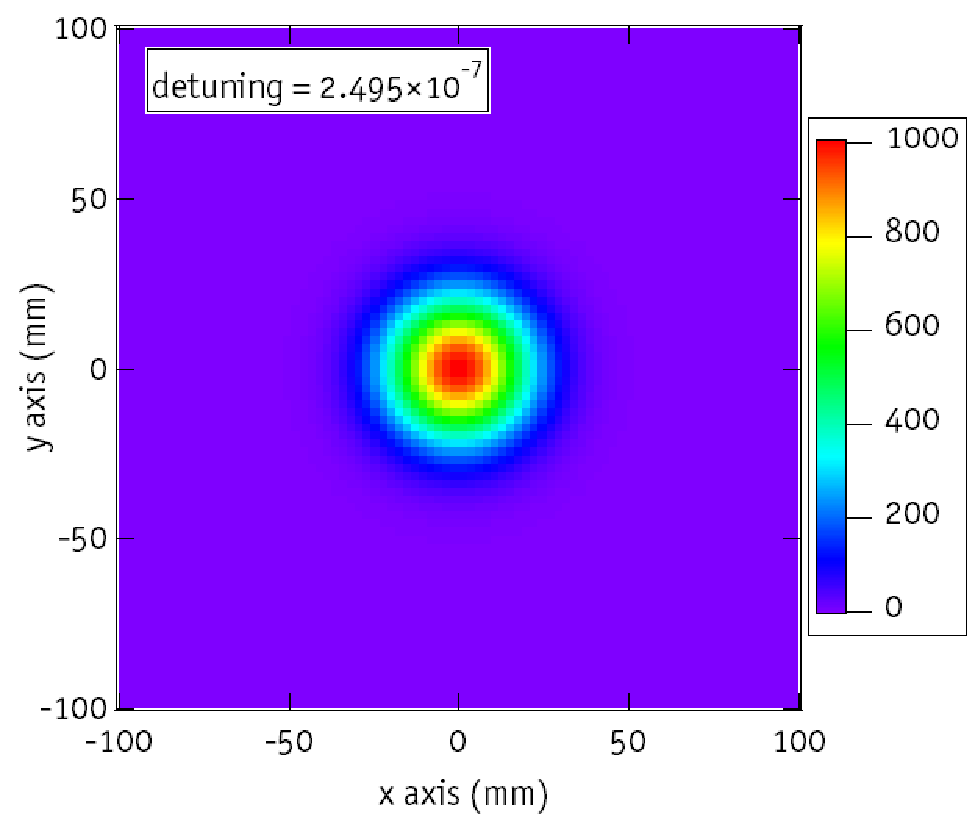
\includegraphics[width = 0.33\textwidth]{Fig2_mode3.pdf}\hfill
\end{center}
\caption{\label{fig2:HOM} 2D amplitude of the circulating field responsible for the 3 peaks in the plot of the cavity circulating as a function of the detuning (figure \ref{fig2:cavres}). We can recognise from left to right the mode LG$_{10}$, LG$_{20}$ and finally the fundamental mode LG$_{00}$. The presence of the there first LG$_{m0}$ optical modes indicates that the input beam is properly aligned with the cavity axis but we have a slight mode mismatching. }
\end{figure}

\section{Calculating the circulating field}
\label{sec2:4}
The previous procedure \textcolor{blue}{Find\_resonance\_length.m} is essential to determine the operating point for the cavity. In most cases the cavity is locked on the fundamental mode TEM$_{00}$, so the procedure \textcolor{blue}{Find\_resonance\_length.m} returns by default the value of the detuning required to make the TEM$_{00}$ resonant inside the cavity. It is always implicitly assumed that the maximum circulating power is obtained for a resonant TEM$_{00}$ and not for a higher order optical mode.\\

After we have calculated the resonance length, the script \textcolor{blue}{Get\_results.m} can be called. This script calculates the static fields in the Fabry perot cavity and displayed the total circulating power as well as other results.\\

The procedure to calculate the circulating field was explained in the section \ref{sec1.4} and is briefly reminded here. First the input laser field (variable \emph{Field.Start} in OSCAR) crosses the input test mass substrate, creating the intermediate circulating field (variable \emph{Field.Circ} and also called $E_1$ in figure \ref{fig1:cavity}). Then the intermediate circulating field is propagated back and forth between the cavity mirrors with the number of round trip determined by the variable \emph{Iter.final}. The total circulating field (variable \emph{Field.Total}) is derived by summing all the field intermediate field at a defined position in the cavity, in OSCAR it is done after the reflection from the input mirror. Everything described above can be simply achieved in Matlab as shown in the listing \ref{lis2:cav_circ}.\\

\begin{lstlisting}[float=htp,caption=The core of the OSCAR programm to calculate the circulating field in a cavity\label{lis2:cav_circ},frame=lines]

Length.reso_zoom = 8.7794200e-007;
Iter.final = 3000;

Phase_shift =  exp(i*Laser.k_prop* Length.reso_zoom);

Field.Circ = Propa_mirror(Field.Start, Mirror.ITM_trans,i*ITM.t);

for q = 1:Iter.final

    Field.Total = Field.Total + Field.Circ;

    Field.Circ = Make_propagation(Field.Circ,Mat_propagation);
    Field.Circ = Propa_mirror(Field.Circ,Mirror.ITM_cav,ETM.r);
    Field.Circ = Make_propagation(Field.Circ,Mat_propagation);
    Field.Circ = Field.Circ * Phase_shift;
    Field.Circ = Propa_mirror(Field.Circ, Mirror.ITM_cav,ITM.r);

end

\end{lstlisting}

After the calculation of the total circulating field in the cavity \emph{Field.Total}, the transmitted beam \emph{Field.Transmit} and the reflected beam \emph{Field.Reflect} can be easily derived. The transmitted beam is simply the total circulating field after a transmission through the end mirror. The reflected beam is the sum of the input field directly reflected by the input mirror and the field leaking from the cavity (which is the total circulating field transmitted by the input mirror).\\

\section{Displaying the results}
\label{sec2:5}
After the total circulating field, the transmitted field and the reflected field have been calculated, the results can be displayed. First some parameters (with obvious names) are written in the Matlab command window, then a 2D plot of the different optical fields present is displayed as shown in figure \ref{fig2:display}.

\begin{verbatim}
 ------ Display the results ------
 Circulating power (W): 749.256602
 Reflected power (W): 0.885891
 Transmitted power (W): 0.037463
 Beam radius on the ITM (m): 0.020574
 Beam radius on the ETM (m): 0.020577
 Cavity waist size (m): 0.016462
 Location of the waist from ITM (m): -499.853070
\end{verbatim}

\begin{figure}
\begin{center}
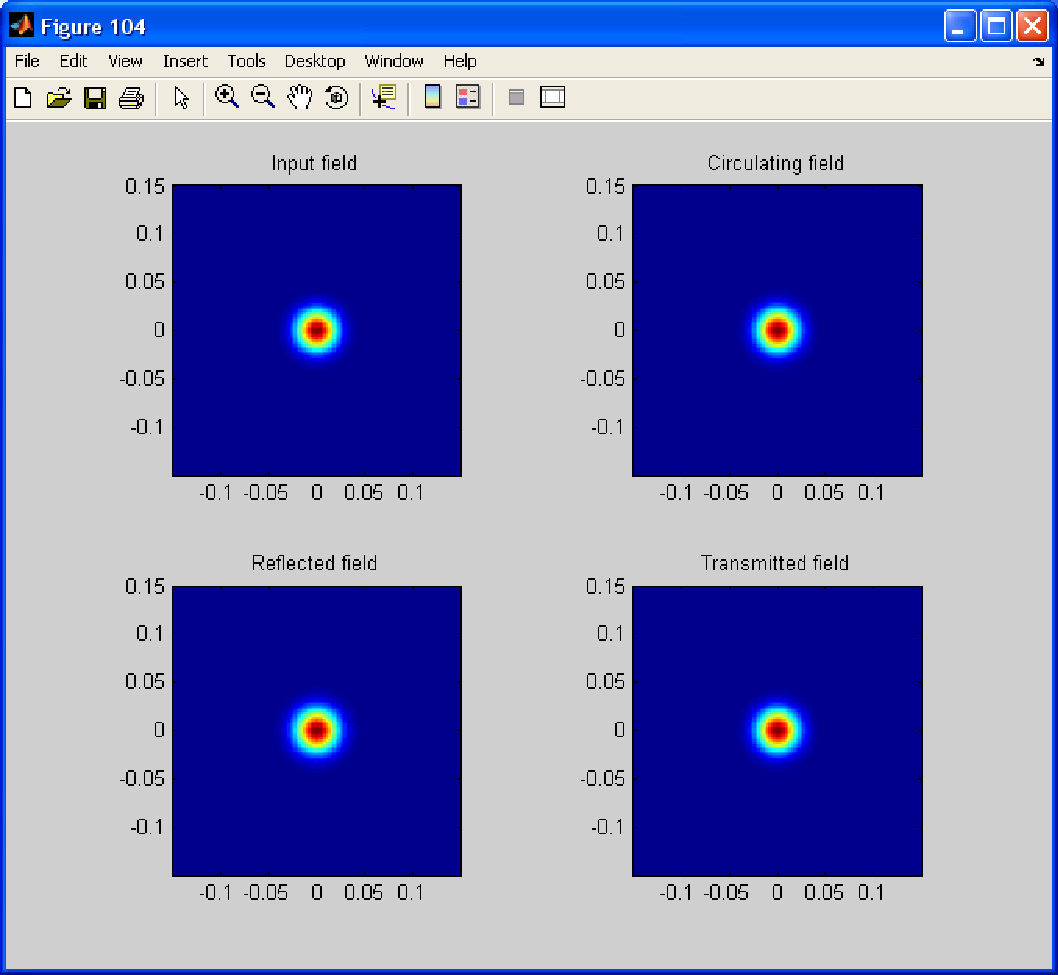
\includegraphics[width = 0.75\textwidth]{Fig2_results.pdf}
\end{center}
\caption{\label{fig2:display} Amplitude profile of the different steady state optical fields in the Fabry Perot cavity. }
\end{figure}

To feel confident in the results from OSCAR, it is always good to test the results with different parameters for the number of light round trip or the size of the grid. If the results are very sensitive to one parameters, it usually means that there is a problem somewhere, and further checks are required.

For example, the results as a function of number of light round trip are presented in the table \ref{tab2:RT}. As expected on resonance, the circulating power, defined by the power of the sum of all the fields $E_i$ increases when the number of field $E_i$ computed increases. The right number of iteration to consider for a simulation depends on the finesse of the cavity. For a low finesse cavity, with a high round trip loss, the power contained in the field $E_i$ will quickly decrease and rapidly becomes negligible after few round trips. In table \ref{tab2:RT}, the FFT results are compared with the results from the software Finesse \cite{Finesse}, which is based on mode expansion. The Finesse script used to simulate the Fabry Perot cavity is presented in appendix \ref{chaB}.\\

\begin{table}[tbp]
  \centering
  \caption{\label{tab2:RT} Influence of the total number of light round trip considered (variable \emph{Iter.final}) on the results. The size of the grid is set to 128 $\times$ 128.}
\begin{tabular}{|l|c|c|c|}
\hline
Number of  & Circulating & Cavity waist & Cavity waist \\
iteration &  power (W) & size (mm) &  position from IM (m) \\
\hline
1000 &  640.712 &  18.403 & -499.835 \\
2500 &  747.546 &  18.403 & -499.852 \\
5000 &  749.903 &  18.403 & -499.853 \\
10000 &  749.906 &  18.403 & -499.835 \\
\hline
\hline
Finesse &  749.906 &  18.403 & -500 \\
\hline
\end{tabular}
\end{table}

Another important parameter to test is the resolution of the grid. The results for different sizes of the grid are presented in the table \ref{tab2:grid_size}. As we can see the results are pretty robust even with a coarse grid. For a grid size of 32 $\times$ 32, the grid resolution is 1~cm, which means the beam radius is just represented by 2 pixels in the cavity. Even with such a low resolution, the results are still accurate.

\begin{table}[tbp]
  \centering
  \caption{\label{tab2:grid_size} Influence of the size of the grid (variable \emph{Grid.Num\_point}) on the results. The number of iteration is 5000. The computation time is normalised by the computation time required for a grid of size 128 $\times$ 128 (which is less than 2 minutes on a modern computer).}
\begin{tabular}{|l|c|c|c|c|}
\hline
Size of   & Circulating & Cavity waist & Cavity waist & Normalised \\
the grid &  power (W) & size (mm) &  position from IM (m) & computation time\\
\hline
32 $\times$ 32 &  749.902 &  18.403 & -499.854 & 0.09 \\
64 $\times$ 64 &  749.903 &  18.403 & -499.853 & 0.31 \\
128 $\times$ 128 &  749.903 &  18.403 & -499.853 & 1.00 \\
256 $\times$ 256 &  749.902 & 18.403 & -499.844 & 7.32\\
\hline
\hline
Finesse &  749.906 &  18.403 & -500 & - \\
\hline
\end{tabular}
\end{table}


%Circulating field
%
%?Other field
%
%
%
%More points
%
%comparison finesse result, size of the grid, finesse
%
%equivalent finesse file in annexe

%128 * 128
% Nb iter     Pcirc      Pref       Beam size ITM Cavity waist    Waist position
% 1000
% 2500
% 5000
% 10000
%
%10000
%Circulating power (W): 749.906250
% Reflected power (W): 0.887468
% Transmitted power (W): 0.037495
% Beam radius on the ITM (m): 0.020574
% Beam radius on the ETM (m): 0.020577
% Cavity waist size (m): 0.018403
% Location of the waist from ITM (m): -499.853070
%
% 5000
%  Circulating power (W): 749.902530
% Reflected power (W): 0.887459
% Transmitted power (W): 0.037495
% Beam radius on the ITM (m): 0.020574
% Beam radius on the ETM (m): 0.020577
% Cavity waist size (m): 0.018403
% Location of the waist from ITM (m): -499.853070
%
% 2500
%
%  Circulating power (W): 747.545912
% Reflected power (W): 0.881741
% Transmitted power (W): 0.037377
% Beam radius on the ITM (m): 0.020574
% Beam radius on the ETM (m): 0.020577
% Cavity waist size (m): 0.018403
% Location of the waist from ITM (m): -499.852995
%
% 1000
% Circulating power (W): 640.712171
% Reflected power (W): 0.633378
% Transmitted power (W): 0.032036
% Beam radius on the ITM (m): 0.020574
% Beam radius on the ETM (m): 0.020577
% Cavity waist size (m): 0.018403
% Location of the waist from ITM (m): -499.835107
%
% 5000 iter
%
% 64*64
% Circulating power (W): 749.902653
% Reflected power (W): 0.887459
% Transmitted power (W): 0.037495
% Beam radius on the ITM (m): 0.020574
% Beam radius on the ETM (m): 0.020577
% Cavity waist size (m): 0.018403
% Location of the waist from ITM (m): -499.853236
%Elapsed time is 34.988457 seconds.
%
%32*32
% Circulating power (W): 749.902499
% Reflected power (W): 0.887459
% Transmitted power (W): 0.037495
% Beam radius on the ITM (m): 0.020574
% Beam radius on the ETM (m): 0.020577
% Cavity waist size (m): 0.018403
% Location of the waist from ITM (m): -499.854544
%Elapsed time is 10.540556 seconds.
%
%128*128
% Circulating power (W): 749.902530
% Reflected power (W): 0.887459
% Transmitted power (W): 0.037495
% Beam radius on the ITM (m): 0.020574
% Beam radius on the ETM (m): 0.020577
% Cavity waist size (m): 0.018403
% Location of the waist from ITM (m): -499.853070
%Elapsed time is 111.589948 seconds.
%
%256*256
%Circulating power (W): 749.902387
% Reflected power (W): 0.887459
% Transmitted power (W): 0.037495
% Beam radius on the ITM (m): 0.020574
% Beam radius on the ETM (m): 0.020577
% Cavity waist size (m): 0.018403
% Location of the waist from ITM (m): -499.844147
%Elapsed time is 817.170512 seconds.

\section{Calculating the cavity eigen-mode and diffraction loss}
\label{sec2:6}
We can first wonder what is called a cavity eigen-mode ? A cavity eigen mode is an electric field which comes back exactly with the same spatial profile after one cavity round trip. The spatial profile must be identical but not necessary the amplitude since the cavity may be lossy. The usual cavity eigen modes are the set of Hermitte-Gauss and Laguere-Gauss for cavity with spherical mirrors, as most of the readers must already know.

For high finesse cavity\footnote{Quantitatively (and approximatively), we could say that a cavity has a high finesse when the the circulating power is much higher than the input power}, the circulating field is in fact a cavity eigen mode. This can be easily understood if the input cavity field is negligible in front of the cavity circulating field, a more rigorous demonstration can be found in \cite{Saha:97} for example. Mode cleaner cavities are based on this principle, the transmitted beam is the TEM$_{00}$ cavity eigen-mode, whereas the input beam may be composed of several optical modes.

Usually, we seldom need a FFT code to calculate the eigen modes of a Fabry Perot cavity with spherical mirrors since the exact analytical solutions are known \cite{Koechner}. However, we may want to know the cavity eigen modes if the mirrors are not perfectly spherical (because of thermal lensing) or if beam clipping due to finite size mirrors is important. To know the cavity eigen modes in this case, we defined an input beam close in shape to the supposed cavity eigen modes and then calculate the cavity circulating field. The cavity circulating field will be the cavity eigen mode. Some problems may arise if the cavity is nearly degenerated and the input beam is composed of several resonant or near resonant modes. In this case we can think of two solutions:
\begin{enumerate}
  \item Increase the cavity finesse to have a better separation between optical modes and if necessary generate some specific losses to attenuate the undesirable optical modes.
  \item Take the cavity circulating field as a new input field and start a new calculation. This step can be done several times and could be understood as cascading optical cavities to increase the mode cleaning effect.
\end{enumerate}

Since we have now an idea about how to calculate a cavity eigen mode, we can also try to calculate the diffraction loss for this mode. We called diffraction loss, the loss due to the finite size of the mirrors. This loss is also sometime referred as clipping loss. Since in theory, Gaussian beams have an infinite spatial extend, diffraction losses are always present. However the loss can become negligible for large diameter mirrors and
small laser beam radius. For example, the diffraction loss of a laser beam of beam radius 6~cm after reflection on a 15~cm radius mirror is only 4~ppm \cite{Siegman}. The diffraction loss are more important for higher order optical modes and ultimately can even affect the profile of the mode \cite{Pab}.\\

In OSCAR the diffraction loss of an eigen mode is computed by calculating the round trip loss of the mode when the reflectivities of the cavity mirrors are set to 1. So the first step is to calculate the cavity eigen mode, this is usually done by calculating the circulating field in a high finesse cavity. The second step is to normalised the power of the eigen mode to 1 and then propagate the mode one round trip in the cavity whose mirrors reflectivities are set to 1. Finally, the diffraction loss is simply the power lost by the mode during one round trip. The above steps are shown in the listing \ref{lis2:diffloss}.

\begin{lstlisting}[float=tp,caption=Piece of code used to calculate the diffraction loss. We suppose that we have already calculate the circulating field \emph{Field.Total}. \label{lis2:diffloss},frame=lines]
% Normalise the circulating field (=the eigen-nmode)
Field.loss = Field.Total;
Field.loss = Field.loss/sqrt(Calculate_power(Field.loss));

% Make a round trip with a reflectivity of 1 for the mirrors
Field.loss = Make_propagation(Field.loss,Mat_propagation);
Field.loss = Propa_mirror(Field.loss,Mirror.ETM_cav,1);
Field.loss = Make_propagation(Field.loss,Mat_propagation);
Field.loss = Propa_mirror(Field.loss, Mirror.ITM_cav,1);

% Calculate the diffraction loss
Dif_loss = (1 - Calculate_power(Field.loss));
fprintf('Diffraction loss per round trip: %d \n',Dif_loss);
\end{lstlisting}

An example about how to calculate diffraction loss with OSCAR can be found in the folder called \textcolor{blue}{Calculate\_diffraction\_loss}. This example is detailed in the chapter \ref{cha3.2} of this manual.

\section{A typical OSCAR run}

A typical run of OSCAR consists of running consecutively three different Matlab scripts:

\begin{enumerate}
  \item \textcolor{blue}{CreateField.m}, is the script used to initialised the variables and defined the optical cavity parameters, the mirror maps as well as the input beam.
  \item \textcolor{blue}{Find\_resonance\_length.m} is used to find automatically the resonance length of the cavity which maximise the circulating power. In most cases, the resonance length locks the cavity on the TEM$_{00}$. Manually it is possible to lock the cavity on any arbitrary position, for example to see the resonance of one higher order mode.
  \item \textcolor{blue}{Get\_results.m} is the main procedure which get the circulating field in the cavity and if required also the reflected and transmitted fields and the diffraction loss of the circulating field.
\end{enumerate}

The call for three previous script are usually reunited into one single scrip called \textcolor{blue}{Run\_OSCAR.m}.

\section{Script and function list}

Here the list of Matlab scripts that you may find in every OSCAR folders. Depending on the goal of the simulation, the scripts may not be exactly the same and some variations exist.

\begin{itemize}
  \item \textcolor{blue}{Beam\_parameter.m}, a function which takes for parameter a complex 2D Gaussian field and returns the beam radius and the wavefront radius of curvature. The fit only works for fundamental Gaussian beam but it can easily be adapted to also fit higher order modes.
  \item \textcolor{blue}{Build\_Field\_Cavity.m} is a function used to find the resonance length, see section \ref{sec2:2.2.3}.
  \item \textcolor{blue}{Calculate\_power.m} a simple function which takes a 2D field and returns the optical power of the field.
  \item \textcolor{blue}{CreateField.m}, the first script called in OSCAR to initialise all the variables, see section \ref{sec2:2.2}.
  \item \textcolor{blue}{CreateMirror.m} script to create the matrix representing the wavefront distortion induced by the mirrors, see section \ref{sec1:3:2}.
  \item \textcolor{blue}{Find\_resonance\_length.m} script to find the microscopic detuning required to set the cavity on resonance, see section \ref{sec2:3}.
%  \item \textcolor{blue}{Fit\_Gaussian.m} small function called by \textcolor{blue}{Beam\_parameter.m}. As the name says, the function does a 1D fit of a Gaussian beam at the waist.
  \item \textcolor{blue}{Get\_results.m} main OSCAR procedure to calculate the circulating power in the cavity. The script is also used to do some post processing of the results, see section \ref{sec2:4} and \ref{sec2:5}.
  \item \textcolor{blue}{Make\_propagation.m} propagates a 2D field over a certain distance. The function takes two arguments a field and a propagation matrix and return the field after propagation. The function is the implementation of the last three lines in listing \ref{lis1:start2}.
  \item \textcolor{blue}{Plot\_Field.m}, a function which takes a 2D field and plots the amplitude of the field in 2D (or 3D if it is desired).
  \item \textcolor{blue}{Propa\_mirror.m} a function to simulate the effect of a wavefront distortion. The function takes a 2D input field, a mirror map or any distortion and a reflectivity (or transmission) and returns the field after reflection (or transmission). The function is described in section \ref{sec1:3:5}.
  \item \textcolor{blue}{Propagate\_Field.m} creates the initial 3D matrix used to calculate the circulating field for the different detuning, see section \ref{sec2:2.2.3} for further explanations.
\end{itemize}




\chapter{Applications}

In this chapter, we provide examples of some typical results which can be obtained with OSCAR. These examples could be taken as a starting point to build more complex simulations. The OSCAR scripts associated with each examples are provided in the OSCAR package. The example described here are using the classic version of OSCAR (version 1.X) which can be downloaded here \cite{OS_down}. For new user, it is recommended to use OSCAR V3.0 and so jump directly to the section \ref{ch4:ex}

\section{Distortion of the optical field due to thermal lensing}\label{cha3.1}

Let's consider the same Fabry-Perot cavity as the one described in the previous chapter (section \ref{chap2:1}). Instead of using an input laser beam of 1~W, we upgrade the input power to 500~W (so the circulating power is now 375~kW) and we are interested to simulate some thermal lensing. Both input and end mirrors are supposed to be made of fused silica with a substrate absorption of 2~ppm/cm and a coating absorption of 0.5~ppm.

At least two distinctive effects can be induced due to the optical power absorbed in the mirrors:
\begin{itemize}
  \item A temperature gradient inside the substrates of the mirrors appears. The temperature gradient generates a refractive index gradient (thermo-optic effect) which induces a wavefront distortion for the beam crossing the optics.
  \item Since the temperature is no longer uniform in the test mass, the curvature of the optic surface will change as a result of thermal expansion. In this case we can expect the eigen mode of the cavity to change as well.
\end{itemize}

Before we continue, it is better to make some assumptions to lighten the calculations. If the reader understands the method described here it is straight forward to implement a full model. First we will suppose that we have uniform absorption in the test mass, so we can take advantage of the cylindrical symmetry. The power absorbed is dominated by the coating absorption, so we will only take into account the temperature gradient $T(r,z)$ in the optics and the thermal expansion of the mirror high reflective (HR) coating surface $\delta s(r)$. The deformations of the anti reflective coating are assumed to be negligible.

OSCAR can not simulate directly the effect of the optical absorption. If required an analytical formula can be implemented \cite{Hello321} however it is not as flexible as finite element simulations in particular if thermal lensing compensation scheme has to be investigated. I used the software ANSYS to simulate the temperature gradient $T(r,z)$ in the optics and the thermal expansion of the mirror surface $\delta s(r)$\footnote{We assume uniform absorption in the test mass, so we can take advantage of the cylindrical symmetry.}. A schematic of the hot cavity is shown in figure \ref{fig3:hotcav}.

\begin{figure}
\begin{center}
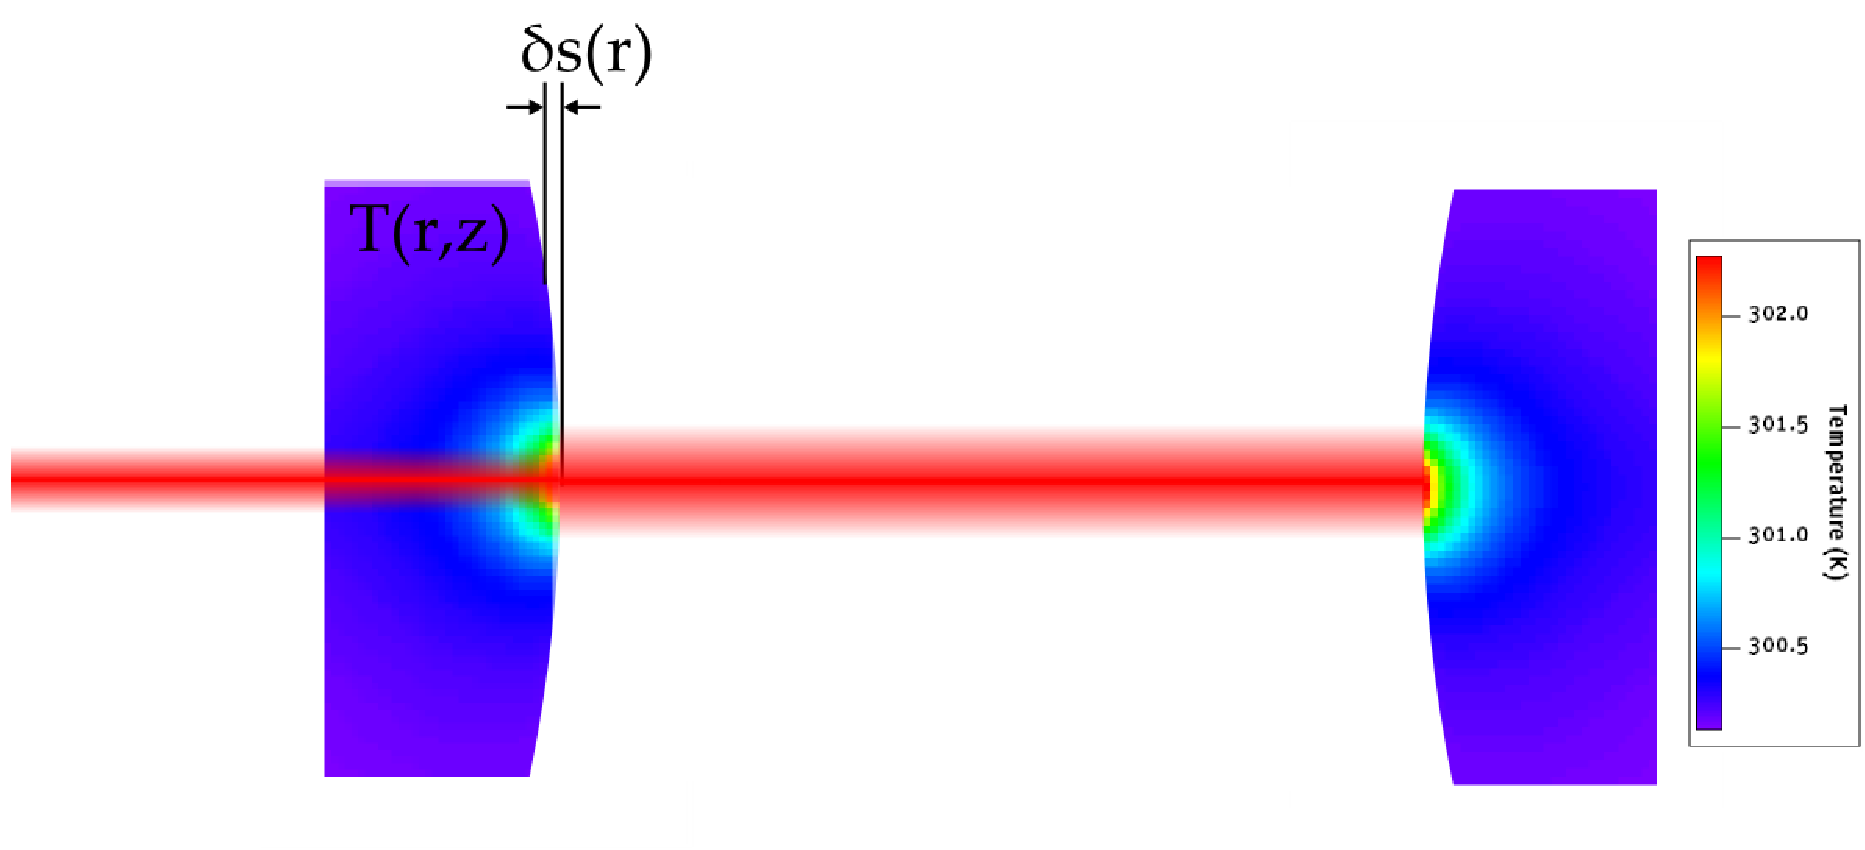
\includegraphics[width = 0.95\textwidth]{Fig3_Hot_cav2.pdf}
\end{center}
\caption{\label{fig3:hotcav} Schematics of the hot cavity. The mirror diameter is 250~mm and the thickness is 100~mm. We can notice that the temperature profile is dominated by the coating absorption. The optical parameters are detailed in the text. For clarity, we did not represent the curvature of the cold optics and we suppose the same distortion in the input and end mirrors. $T(r,z)$ represents the temperature distribution inside the test mass and $\delta s(r)$ the change in sagitta due to the optical absorption.}
\end{figure}

From the temperature distribution inside the substrate and the sagitta change, we can derive the optical path length difference $\Delta OPN_{sub}^{trans}(r)$ induced by the substrate in transmission according to:

\begin{eqnarray}\label{eq3:OPN1}
  \Delta OPN_{sub}^{trans}(r) &=& \int_0^L n(r,z) dz - \int_0^L n(0,z) dz + (n-1)\delta s(r) \nonumber \\
                &=&  \int_0^L \beta T(r,z) dz - \int_0^L \beta T(0,z) + (n-1)\delta s(r) dz
\end{eqnarray}

With $\beta$ the thermo-optic coefficent and n the refractive index of the substrate. Similarly, we can calculate the wavefront distortion $\Delta OPN_{sub}^{ref}(r)$ for the input beam reflected directly reflected on the input mirror:

\begin{equation}\label{eq3:OPN2}
  \Delta OPN_{sub}^{ref}(r) = 2\left( \int_0^L \beta T(r,z) dz - \int_0^L \beta T(0,z) + n\delta s(r) \right)
\end{equation}

And finally, the wavefront distortion of the beam reflected on the mirrors inside the cavity is:

\begin{equation}\label{eq3:OPN3}
  \Delta OPN_{cav}^{ref}(r) = 2 \delta s(r)
\end{equation}

Of course, the three wavefront distortions just defined, have to be added to any wavefront distortion already present when the cavity is cold, especially the ones induced by the curvature of the mirrors. For references, the main distortions due to thermal lensing which have to be included in OSCAR are plotted in figure \ref{fig3:OPN}.\\

Here an example how to proceed in reality. First run ANSYS to simulate the temperature distribution in the test mass as well as the thermal expansion of the optic. Then from these results, we can save a text file with two results, first the wavefront distortion induced by the thermo-optic effect for the optic in transmission and the change in sagitta of the optics. The text file is then loaded in OSCAR and the new wavefront distortions for the all optics of the cavity are calculated accordingly. An example of such a text file is presented below, the first column is the radius, the second the optical path length difference in transmission and the third the change in sagitta, all the columns are in meter.

\begin{verbatim}
 -1.2500000e-001 -1.0824598e-006 -2.6695000e-008
 -1.2142857e-001 -1.0731224e-006 -2.6433549e-008
 -1.1785714e-001 -1.0655394e-006 -2.6172131e-008
 -1.1428571e-001 -1.0577238e-006 -2.5911061e-008
 -1.1071429e-001 -1.0496365e-006 -2.5695000e-008
 -1.0714286e-001 -1.0398661e-006 -2.5695000e-008
 -1.0357143e-001 -1.0304229e-006 -2.5615955e-008
 -1.0000000e-001 -1.0216618e-006 -2.5349271e-008
\end{verbatim}

The file can found in the OSCAR distribution under the name \textcolor{blue}{From\_ANSYS.txt} in the folder \textcolor{blue}{Calculate\_TL\_effect}. A graphical representation of the data file from ANSYS is shown in figure \ref{fig3:OPN}.

% 17*11 cm

\begin{figure}
\begin{center}
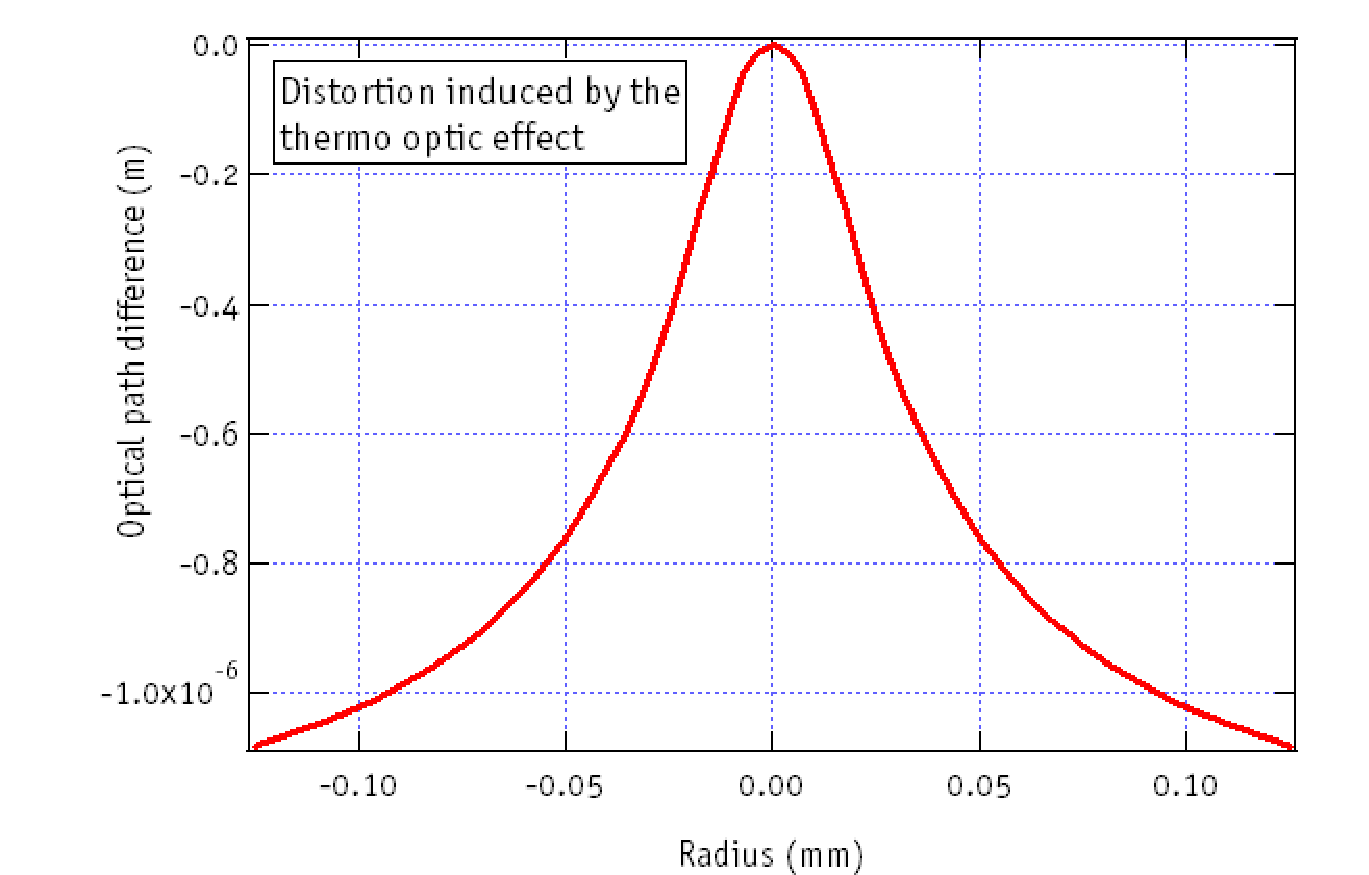
\includegraphics[width = 0.50\textwidth]{Fig3_OPN1.pdf}\hfill
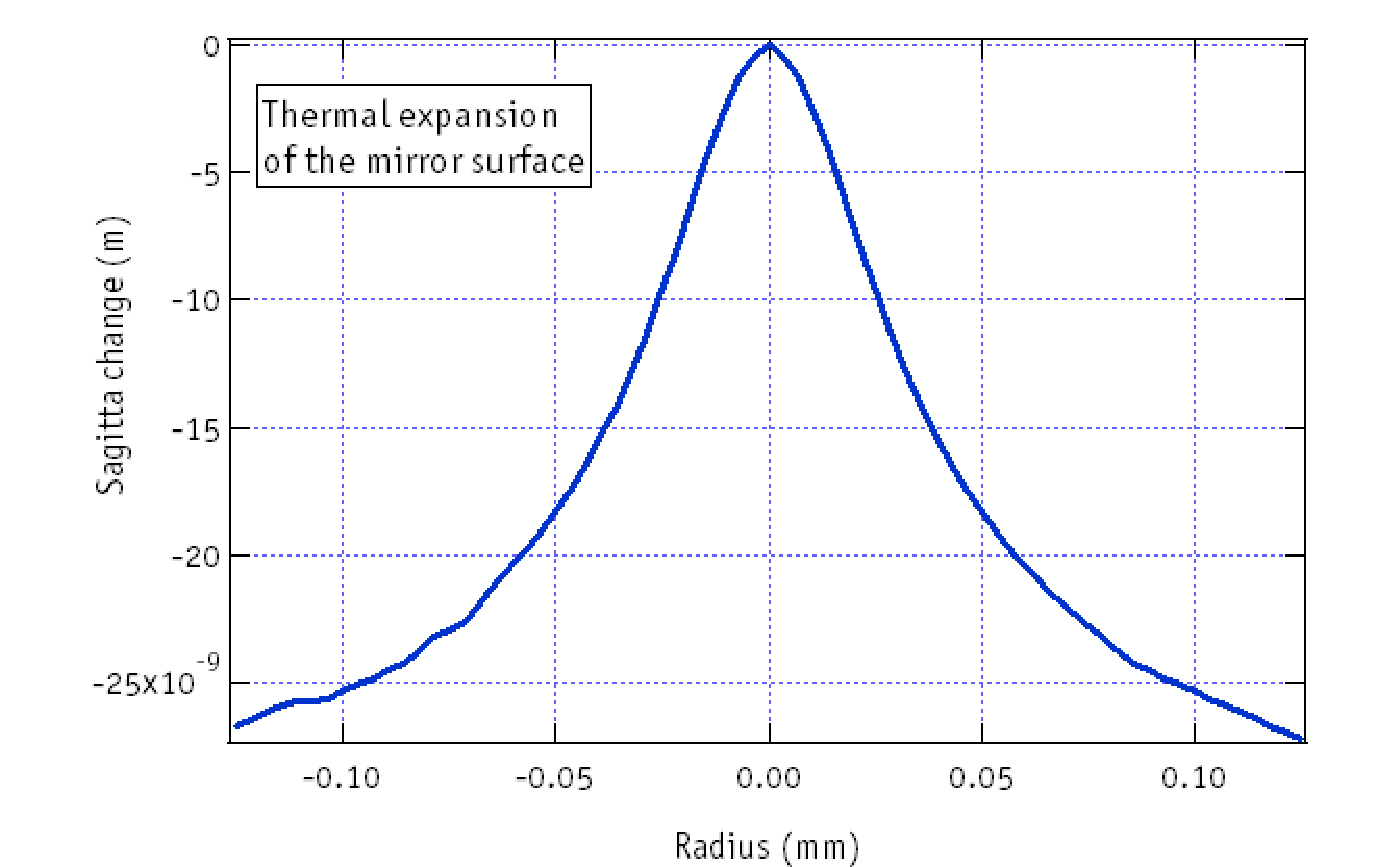
\includegraphics[width = 0.50\textwidth]{Fig3_OPN2.pdf}
\end{center}
\caption{\label{fig3:OPN} Optical path length difference induced by the mirror substrates in transmission when only the thermo optics effect is considered (left) and change in the sagitta of the reflective side of the mirrors (right). It interesting to note the difference between the two vertical scales, the left plot represents an optical path in micrometers, whereas the right plot is in tens of nanometers. These plots are derived from the results of ANSYS simulations and will then be integrated into OSCAR.}
\end{figure}

Most of the time, the resolution used with the results file from ANSYS is different from the grid resolution used in OSCAR so we have to resample the results using an interpolation method. How the results file is integrated into OSCAR is presented into the listing \ref{lis3:read}

\begin{lstlisting}[float=tp,caption=Commands used to read thermal lensing results from ANSYS. \label{lis3:read},frame=lines]
% Load the results file
load('From_ANSYS.txt')
loaded.radius = From_ANSYS(:,1);
loaded.TL = interp1(From_ANSYS(:,1),From_ANSYS(:,2),Grid.D2,'spline')*0.2;
loaded.sag = interp1(From_ANSYS(:,1),From_ANSYS(:,3),Grid.D2,'spline')*0;

% Add the thermal lensing distortion to the previous wavefront
% Special attention to the sign!

Mirror.ITM_cav = Mirror.ITM_cav - 2*loaded.sag;
Mirror.ETM_cav = Mirror.ETM_cav - 2*loaded.sag;

Mirror.ETM_trans = Mirror.ETM_trans + loaded.TL - (Refrac_index-1)*loaded.sag;
Mirror.ITM_trans = Mirror.ITM_trans + loaded.TL - (Refrac_index-1)*loaded.sag;

Mirror.ITM_ref = Mirror.ITM_ref + 2*loaded.TL - 2*Refrac_index*loaded.sag;
\end{lstlisting}

After implementing the distorted mirrors, we can calculate the resonance length for the fundamental mode and then calculate the total circulating field. This is done by running successively the scripts \textcolor{blue}{Find\_resonance\_length.m} and \textcolor{blue}{Get\_results.m}. The comparison between the cold cavity is presented in table \ref{tab3:res}.

\begin{table}[tbp]
  \centering
  \caption{\label{tab3:res} Comparison of the cavity gain and size of the beam on the input mirror for a cavity with and without thermal lensing.}
\begin{tabular}{|l |c|c|}
\hline
{\large\strut} & Cold cavity & Hot cavity \\
\hline
{\large\strut} Cavity gain & 749.3 & 444.8 \\
{\large\strut} Beam radius on IM (mm)& 20.6 & 20.8 \\
\hline
\end{tabular}
\end{table}

Some very interesting points can be deduced by understanding the two lines of the table \ref{tab3:res}:

\begin{itemize}
  \item Due to thermal lensing, the beam radius only increases by 1~\%. That indicates that the mirror profiles are only slightly affected by thermal lensing since the cavity eigen modes are very similar for both cases: cold and hot cavities. This is not a surprise since the change in sagitta of the reflective sides of the mirrors is relatively small as we have previously seen.
  \item The decrease in the optical gain is quite important, since the optical gain is almost divided by a factor 2 between the cold and hot cases. It means in the hot cavity case, we have a strong mode mismatching between the input beam and the cavity fundamental mode. Since the latter has almost not changed, we can deduce that the mode mismatching is induced by the thermal lens in the substrate of the input mirror.
  \item We have assumed a certain amount of optical power absorbed in the mirror, it was based on the optical power circulating in the cold cavity. But since the circulating has decreased due to the mode mismatching, our thermal lens calculating wrong. A simple iterative process can be written to solve this problem and find the steady state parameters.
  \item This simple example shows that in our fused silica mirrors, the main thermal lensing effect is due to the thermal lens in the substrate of the input mirror generated by the optical absorption in the high reflective coating. The conclusion may be different for different substrates such as sapphire or calcium fluoride.
\end{itemize}

\section{Calculating diffraction losses}
\label{cha3.2}

One of the most promising application of FFT optical codes is to calculate the diffraction loss of the circulating cavity field. The method used to calculate the diffraction loss has been explained in section \ref{sec2:6}. An example how to calculate the diffraction loss of the mode HG$_{10}$ is presented in the folder \textcolor{blue}{Calculate\_diffraction\_loss}.

The diffraction loss calculation can be decomposed into three steps:
\begin{enumerate}
  \item Find the resonance length of the cavity for the mode HG$_{10}$. For that we can inject a mode HG$_{10}$ and maximise the circulating power. This approach is too easy, instead we will inject a uniform pattern of light and excite all the optical modes HG$_{m0}$. Then we will select manually the resonance length of the mode HG$_{10}$ in the spectrum of the cavity.
  \item Find the HG$_{10}$ eigen mode of the cavity. The shape of this mode can be different from the theory if the mode undergoes some serious clipping.
  \item Calculate the diffraction loss as the power lost during one light round trip with perfect reflective mirror.
\end{enumerate}

We decide to not inject directly a mode HG$_{10}$ (right plot on figure \ref{fig3:strip}) but instead inject a simpler light pattern which will excite all the optical modes along the horizontal axis. This pattern is one vertical strip with positive amplitude and one vertical strip with negative amplitude as shown in the left plot figure \ref{fig3:strip}.\\

\begin{figure}
\begin{center}
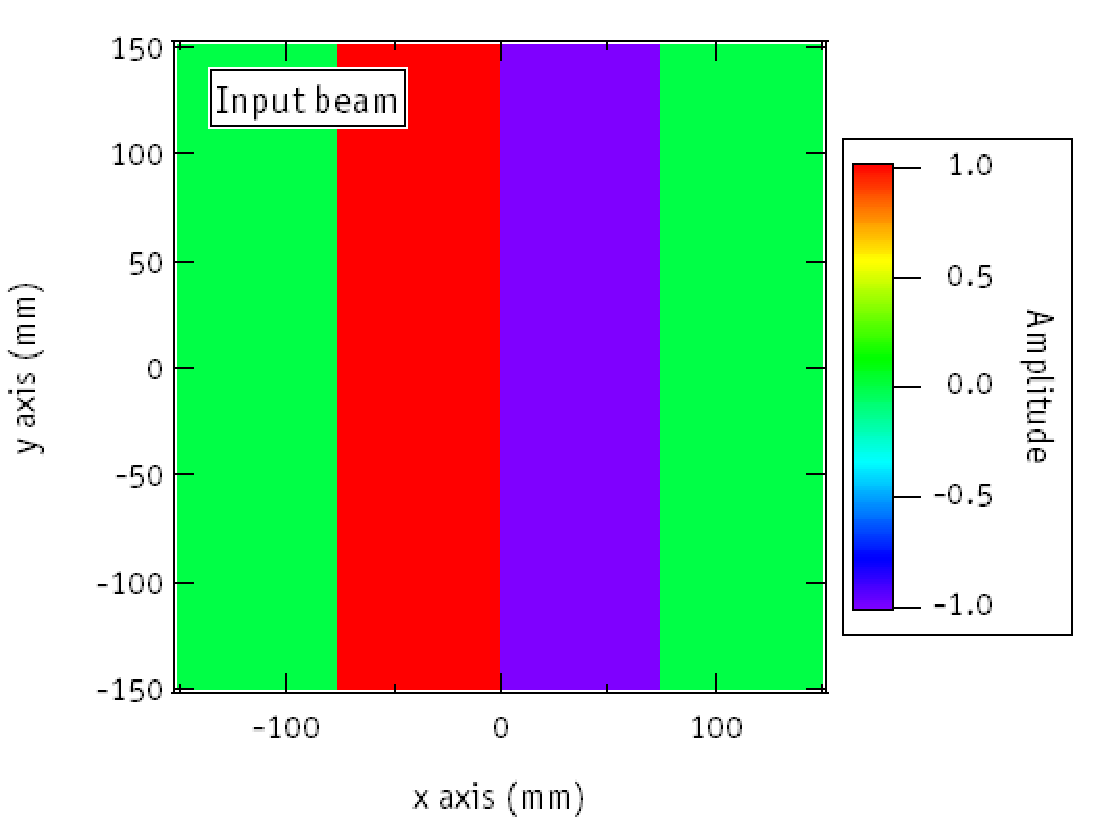
\includegraphics[width = 0.50\textwidth]{Fig3_inputbeam.pdf}\hfill
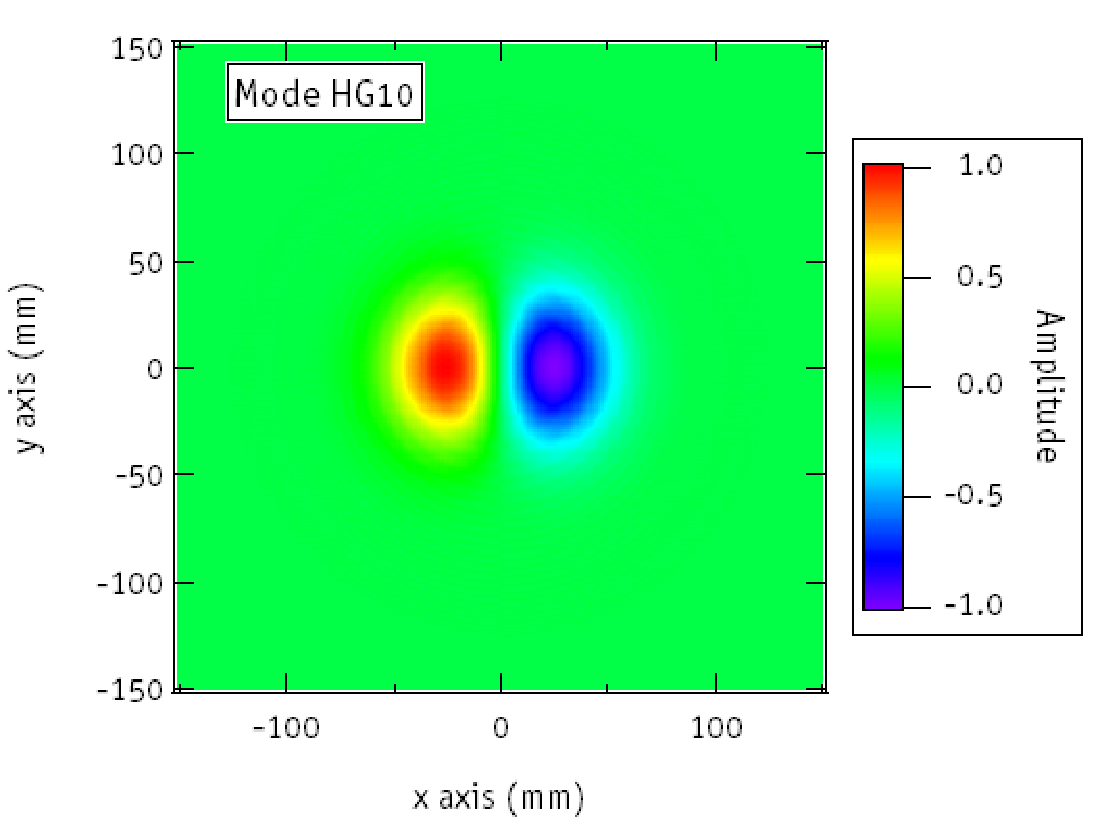
\includegraphics[width = 0.50\textwidth]{Fig3_HG10.pdf}
\end{center}
\caption{In the left plot, is the profile of the input electric field that we inject in the cavity to excite the HG$_{10}$ shown on the right. Both optical pattern are normalised in amplitude.\label{fig3:strip}}
\end{figure}

By using the procedure \textcolor{blue}{Find\_resonance\_length.m}, we can calculate all the cavity modes excited due to our particular input beam. The circulating power as the cavity is scanned over one FSR is shown in figure \ref{fig3:cav_spec}. Each peak in this plot represents the resonance of one of the cavity mode. We can display different cavity eigen modes for the first four highest peaks and we found that the mode HG$_{10}$ resonates for a detuning of $3.181\times 10^{-7}$~m.

\begin{figure}
\begin{center}
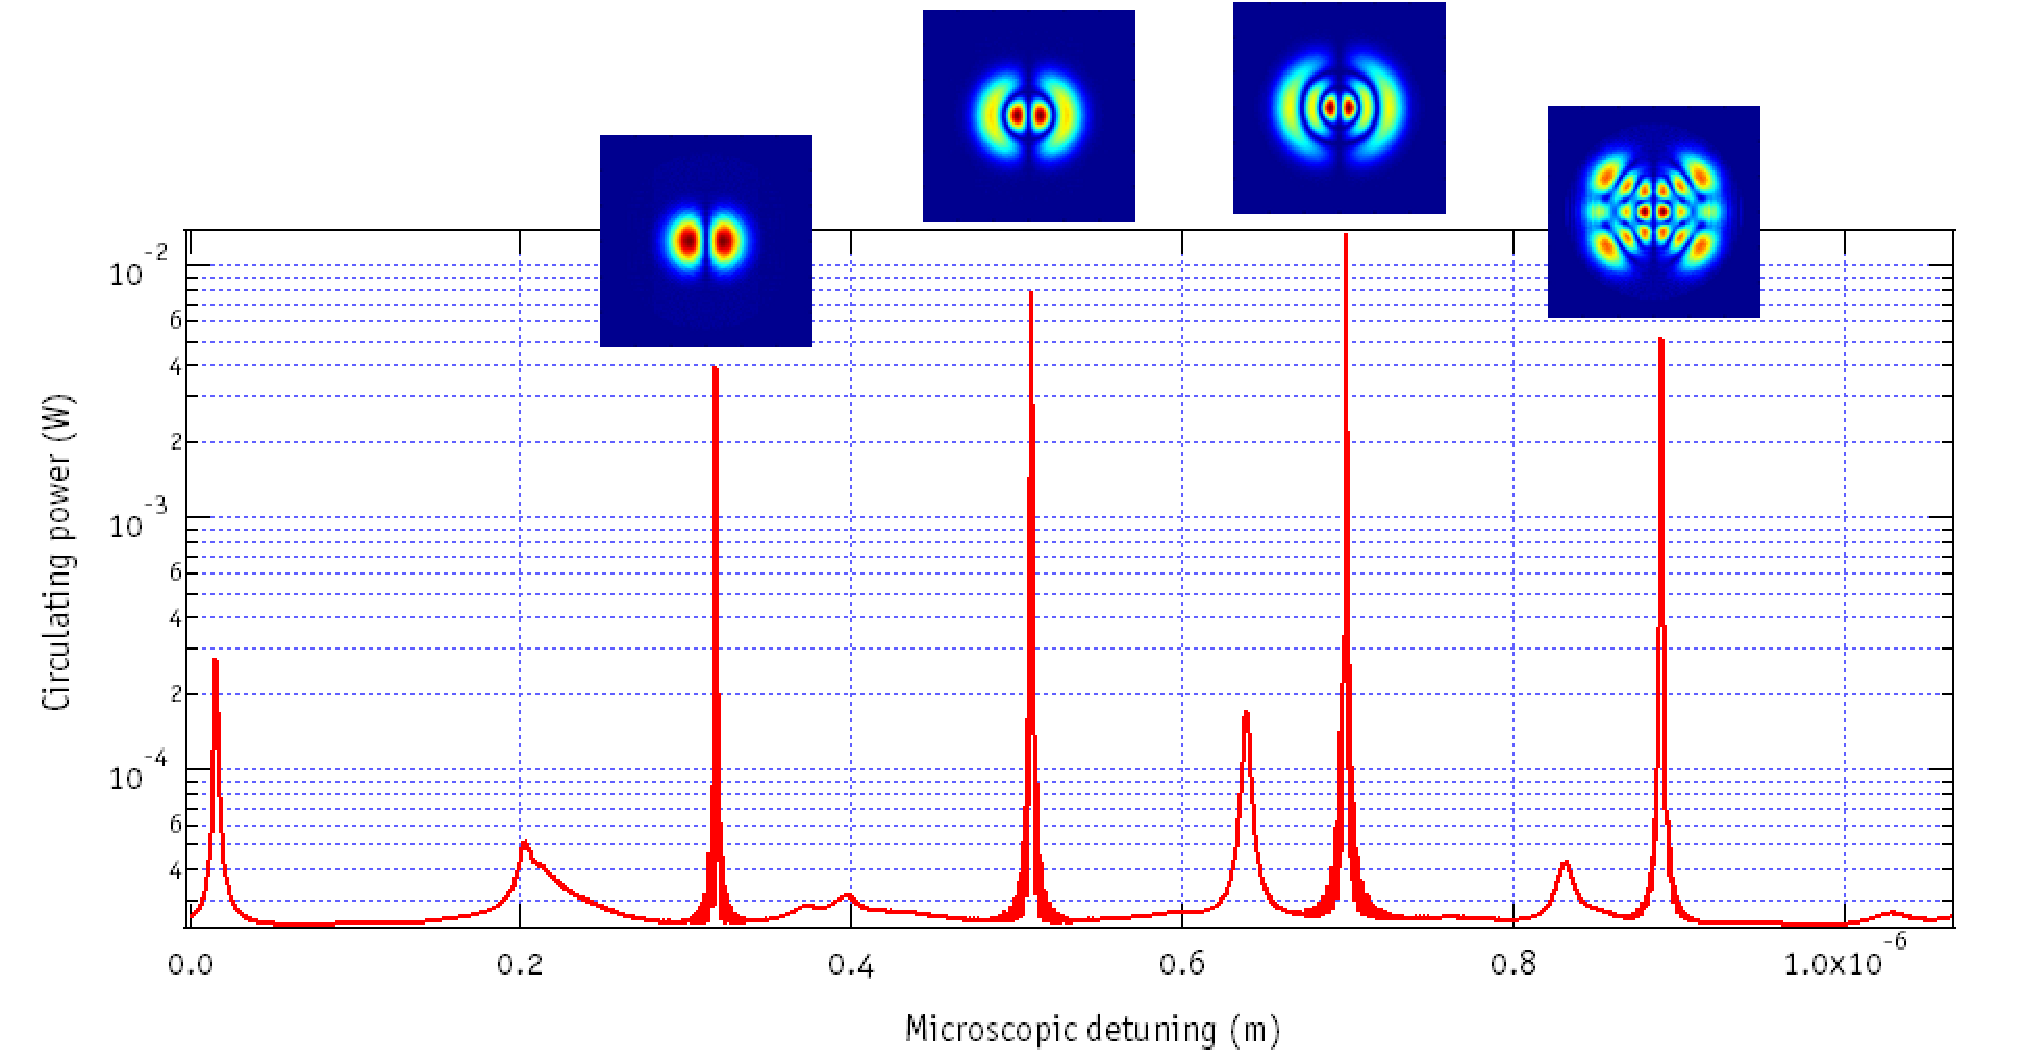
\includegraphics[width = 1\textwidth]{Fig3_Spectrum.pdf}
\end{center}
\caption{Cavity spectrum showing the different resonance lengths of the optical modes. The power profile of the main optical modes is presented above their respective resonance peaks.\label{fig3:cav_spec}}
\end{figure}

Since we have found the resonance length for the mode HG$_{10}$, we can now use the procedure \textcolor{blue}{Get\_results.m} to calculate the diffraction loss using the method described in section \ref{sec2:6}. As the result we found the diffraction loss equal to 618 ppm per round trip. Important beam clipping can also change the shape of the eigen mode of the cavity, this can be easily demonstrated using a FFT code\cite{Pab}.

We can now check how the diffraction loss depends of the size of the grid. The results are shown in \ref{tab3:grid_size}. As we can see the results do not change as we increase the size of the grid (which is a good sign). Below a grid size of 128 $\times$ 128, no realistic eigen modes can be found in the cavity.

\begin{table}[tbp]
  \centering
  \caption{\label{tab3:grid_size} Influence of the size of the grid on the diffraction loss).}
\begin{tabular}{|l|c|}
\hline
{\large\strut} Size of the grid  & Diffraction loss (ppm) \\
\hline
{\large\strut} 128 $\times$ 128 &  618 \\
{\large\strut} 256 $\times$ 256 &  620 \\
{\large\strut} 512 $\times$ 512 &  621 \\
\hline
\end{tabular}
\end{table}



\section{Using flat beams}
\label{cha3.3}

In this section, we will show how OSCAR can be used to calculate the frequency separation between higher order modes. This is in fact an indirect calculation of the Gouy phase shift between optical modes. To make the example more interesting, we will not use the usual Gaussian beams but flat beams. As a consequence of using flat beams, the mirrors of our cavity will no longer have spherical profiles \cite{Flat}.\\

To create the mirror profiles, we will not use directly the analytical formula which is relatively complicated, but instead we will use the wavefront curvature of the flat beam at the mirror position. Since the flat beam is an eigen mode of the cavity, the curvature of the mirrors must match the wavefront of the incoming beam. So the three steps to calculate will be:

%http://scitation.aip.org/getabs/servlet/GetabsServlet?prog=normal&id=PRVDAQ000074000008082002000001&idtype=cvips&gifs=yes


\begin{enumerate}
  \item Use the simple analytical formula to define the flat beam at the waist of the cavity. Since both mirror will have identical profile, we know that the waist position is in the middle of the cavity.
  \item Propagate the beam along half the cavity length, so the flat beam is now at the mirror position.
  \item Calculate the wavefront curvature of the beam at the mirror and then set the mirror profile to be identical to the wavefront.
\end{enumerate}

The method described in the three points above can be directly implemented in OSCAR as shown in the listing \ref{lis3:FB}.

\begin{lstlisting}[float=btp,caption=Script to create the mirror profiles used to support a given light field \label{lis3:FB},frame=lines]
%---------------------- Create nearly concentric flat beam -------------------
% Create the profile at the cavity waist

waist_0 = sqrt((Laser.lambda  * Length_cav) / (2*pi));
p = 3*waist_0; % Defined the width of the Mesa beam

x_temp = Grid.D2/waist_0;
Field.mesa_tmp = (1./x_temp).*exp(-x_temp.^2).*besselj(1,2*x_temp*p/waist_0);

clear('x_temp')

% Propagate the beam from the waist to the mirror
Field.On_mirror = Make_propagation(Field.mesa_tmp,Mat_propagation_h);

% Take the phase of the beam at the mirror and calculate the equivalent
% change in sagitta
Mirror.ETM_cav = (2/Laser.k_prop)*angle(Field.On_mirror);
Mirror.ITM_cav = Mirror.ETM_cav;

\end{lstlisting}


Since we are just interested in the frequency difference between 2 eigen modes of the cavity (and not in the cavity circulating power), the input laser beam only needs to be slightly matched to the cavity eigen modes (and we must have a high finesse to achieve a good mode selection). The important point is that the input beam couples (or excites) at least to the two cavity eigen modes of interest.

As for the input light field, we decided to use a classic fundamental Gaussian beam. By this way we will couple to most the cavity eigen modes which are circularly symmetric, e.g. the equivalent of the LG$_{m0}$ modes. For example the spectrum of the cavity as we scan over one wavelength is shown in figure \ref{fig3_mesa_spec}. As expected we managed to excite the fundamental mode and also some other higher order modes.

\begin{figure}
\begin{center}
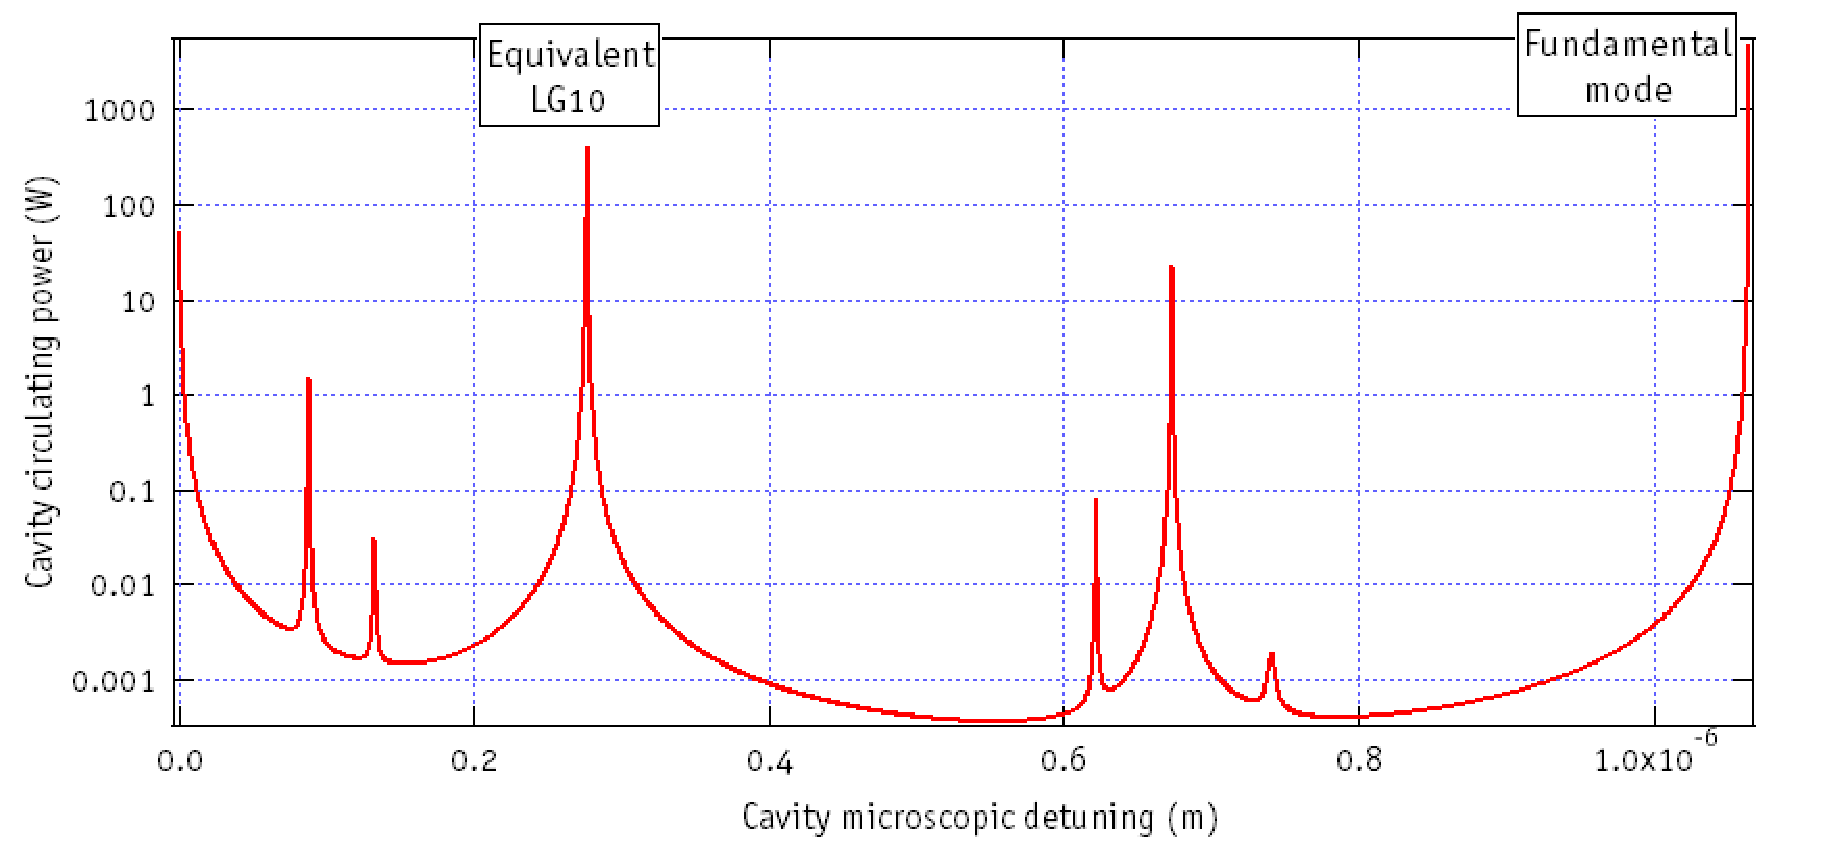
\includegraphics[width = 0.9\textwidth]{Fig3_mesa_spec.pdf}
\end{center}
\caption{Cavity spectrum of the cavity supporting flat beams. It is important to note the fundamental for a detuning of 0. This is not a coincidence, but a direct consequence of the way we defined the mirror profiles (by propagating a beam from the cavity waist).\label{fig3_mesa_spec}}
\end{figure}

Just to have a look, we can display a cross section of the fundamental flat beams and the equivalent LG$_{10}$ to compare the energy distribution. Such a comparison is shown in figure \ref{fig3_mesa_profile}.\\

\begin{figure}
\begin{center}
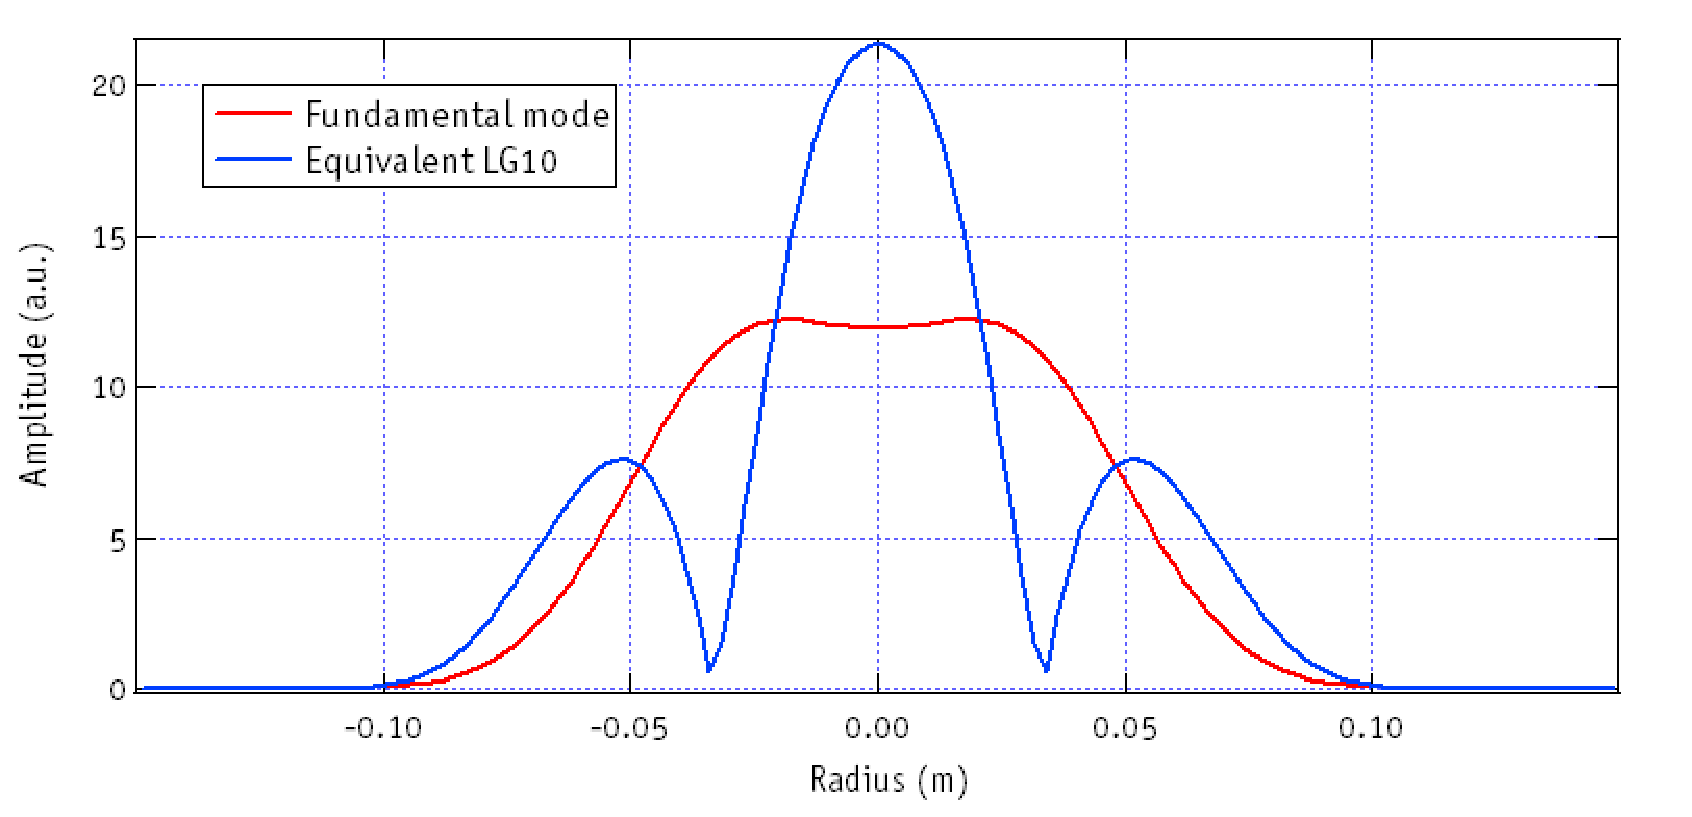
\includegraphics[width = 0.9\textwidth]{Fig3_mesa_profile.pdf}
\end{center}
\caption{Comparison of the profile of the fundamental flat beam with the equivalent LG$_{10}$. Both beam contains the same optical power.\label{fig3_mesa_profile}}
\end{figure}

So we can go back to our initial question what is the frequency separation between the fundamental mesa beam and the mode LG$_{10}$ ? From the spectrum plot, we know the difference of detuning in length between the fundamental mode and the equivalent LG$_{10}$ is $ \Delta l = 2.7664 \times 10^{-7}$~m. Since the displacement of one wavelength $\lambda$ is equivalent to one free spectral range $(c / 2L)$ , the frequency difference $\Delta f$ between the 2 modes is simply:

\begin{equation}
\begin{split}
\Delta f & = (c / 2L) * (\Delta l / \lambda)\\
& = (3 \times 10^8/4000)*( 2.7664 \times 10^{-7} / 1.064 \times 10^{-6}) \\
& = 19.5 \textrm{kHz}
\end{split}
\end{equation}

Using a similar calculation, we could also deduce the Gouy phase shift between the two cavity eigen modes.

\section{Deriving a Pound Drever Hall locking signals}
\label{cha3.4}

In this example, we will show how to implement sidebands in OSCAR. For testing purpose, we can try to derive the Pound Drever Hall (PDH) error signal which is used to lock a Fabry Perot cavity on resonance \cite{PDH}. The error signal is derived in reflection by combining a resonant (or near resonant) carrier field with a non resonant pair of sidebands. In this case, it can be shown that the error signal is in fact proportional to the imaginary part of the reflected field \cite{black:79}. The script for this example can be found in the folder \textcolor{blue}{Calculate\_PDH\_signals}

So the first thing to do, is to create sidebands using a phase modulator. Consider an electric field of amplitude $E_0$ and angular frequency $\omega_0$ incoming on a phase modulator. $E_m$ the electric field after the modulator can be written as:

\begin{equation}
\begin{split}
E_m & = E_0 \exp(i \omega_0 t + m \sin(\omega_m t))\\
    & = E_0 \exp(i \omega_0 t) \sum_{k = -\infty}^{+\infty} (-1)^k J_k(m) \exp(i k \omega_m t) \\
\end{split}
\label{eq3:bessel}
\end{equation}

\begin{table}[tbp]
  \centering
  \caption{\label{tab3:bessel} Values of the first Bessel functions for different modulating indexes m. Conveniently, the Bessel functions follow the property $J_{-k}(m) = (-1)^k J_{k}(m)$ }
\begin{tabular}{|l c c c|l|}
\hline
{\Large\strut} m & 0.1 & 0.2 & 0.4 & Taylor series\\
\hline
{\Large\strut} J$_0$(m) & 0.9975 & 0.9900 & 0.9604 & $1 - \frac{m^2}{4} + \mathcal{O}(x^4)$\\
{\Large\strut} J$_1$(m) & 0.0499 & 0.0995 & 0.1960 & $\frac{m}{2} + \mathcal{O}(x^3)$\\
{\Large\strut} J$_2$(m) & 0.0012 & 0.0050 & 0.0197 & $\frac{m^2}{8} + \mathcal{O}(x^4)$\\
{\Large\strut} J$_3$(m) & 0.0000 & 0.0002 & 0.0013 & $\frac{m^3}{48} + \mathcal{O}(x^5)$\\
\hline
\end{tabular}
\end{table}

With $m$ the modulating index and $\omega_m$ the modulation frequency. $J_k(m)$ is the bessel function of the first kind of order k. For example, the values for the first Bessel functions are shown in table \ref{tab3:bessel}. As a good approximation we can just consider the first order sidebands $k = \pm 1$. So equation \ref{eq3:bessel} can be simplified to:

\begin{equation}
E_m = E_0 \exp(i \omega_0 t) (1 + \frac{m}{2} \exp(i \omega_m t) -  \frac{m}{2} \exp(-i \omega_m t))
\end{equation}

So the electric field after the phase modulator can be expanded as the superposition of three electric fields of angular frequency $\omega_0$ (the carrier) and $\omega_0 + \omega_m$ and $\omega_0 - \omega_m$ (respectively the upper and lower sidebands). Since each field has different frequencies, they will also have different resonant conditions in the cavity.

Consider the sideband with the frequency $\omega_0 + \omega_m$. Propagating over a distance $L$ the sideband undergoes the phase shift $ \exp(i \frac{\omega_0 + \omega_m}{c} L)$. That means, the sideband phase shift is the phase shift of the carrier plus an additional phase shift. Since before entering the cavity, the carrier and the sidebands have the same spatial profile, we can simulate the sidebands in the cavity by taking the simulated carrier and by adding an extra phase shift.\\

Practically, to simulate the carrier and the sidebands, we can simulate independently three optical fields, the carrier and the lower and upper sidebands. The three fields can be treated the same way in the simulation, except that they have different round trip phase shift. Below is the three phase shifts for one round trip in the cavity:

%\begin{equation}
\begin{alignat}{2}
    \quad & \exp(i k Length.reso\_zoom) &\quad&   \text{for the carrier} \nonumber \\
    \quad & \exp(i k Length.reso\_zoom) \times \exp(i \frac{\omega_m}{c} 2 Length\_cav) && \text{for the upper sidebands} \nonumber \\
    \quad & \exp(i k Length.reso\_zoom) \times \exp(-i \frac{\omega_m}{c} 2 Length\_cav) && \text{for the lower sidebands}
\label{eq3:sid23}
\end{alignat}
%\end{equation}

As a reminder \textsl{Length\_cav} is the length of the cavity and \textsl{Length.reso\_zoom} is the microscopic tuning used to set the resonance condition for the carrier.

Since we know how to calculate the carrier and the sidebands fields circulating in the cavity, we can also calculate the reflected fields from the cavity. The reflected light is also the superposition of three fields, the reflected carrier, the reflected lower sidebands and the reflected upper sidebands with respective amplitude $E_0^{ref},\ E_-^{ref} \text{ and } E_+^{ref}$. The power $P_{det}$ detected by photodiode placed in reflection will then be:

\begin{equation}
\begin{split}
P_{det} =\ & |E_0^{ref} +  E_-^{ref}e^{-i \omega_m t} + E_+^{ref}e^{i \omega_m t}|^2 \\
     =\ & |E_0^{ref}|^2 + |E_-^{ref}|^2 + |E_+^{ref}|^2\\
    & + \cos(\omega_m t) \Re(E_0^{ref}E_-^{ref \ast}+E_0^{ref \ast}E_+^{ref})\\
    & + \sin(\omega_m t) \Im(E_0^{ref}E_-^{ref \ast}+E_0^{ref \ast}E_+^{ref})\\
    & + 2 \Re(E_+^{ref \ast}E_-^{ref} e^{-i 2\omega_m t})
\end{split}
\end{equation}

With $\Re$ and $\Im$ the real and imaginary part and $\ast$ designates the complex conjugate. The PDH error signal $e_{PDH}$ is derived by demodulating in phase $P_{det}$ and the resulting signal is then low-pass filtered. As a result $e_{PDH}$ can simply be written:

\begin{equation}
e_{PDH} = \Im(E_0^{ref}E_-^{ref \ast}+E_0^{ref \ast}E_+^{ref})
\label{A3:ePDH}
\end{equation}

The Matlab implementation of the method described above is straight forward. We first defined three electric fields: the carrier and then the lower and upper sidebands. Then we propagate each field in the cavity, calculate the reflected field and then plot the error signal using the formula \ref{A3:ePDH}. To make the result more pertinent, we fact scan the cavity over one free spectral range, so we can see the evolution of the error signal across the resonance.\\

To define the sidebands frequency and amplitude we have to define new variables (with self-explaining names) as shown in the script \ref{lis3:SB}.\\

\begin{lstlisting}[float=btp,caption=New variables to define the sidebands frequency and amplitude \label{lis3:SB},frame=lines]
% Frequency of the sidebands in Hertz and modulation index
Sidebands.frequency = 10E6;
Sidebands.modulation = 0.4;

% New carrier amplitude
Laser.amplitude = Laser.amplitude * besselj(0,Sidebands.modulation);
% Amplitude for one of the 2 sidebands
Sidebands.amplitude = besselj(1,Sidebands.modulation);
Ration_amp = Sidebands.amplitude/Laser.amplitude;

% To add the additional phase shift undergone by the sidebands during the propagation
Sidebands.k_prop = 2*pi*Sidebands.frequency/3E8;
\end{lstlisting}

Then we can calculate the three circulating fields in the cavity called \textsl{Field.Total} \textsl{Field.Total\_sidebands\_plus} and \textsl{Field.Total\_sidebands\_minus} using the usual method introduced in section \ref{sec2:4}. The only difference in the algorithm between the propagation of the carrier and the sidebands is the addition of an extra phase shift per round trip for the sidebands as shown in equation \ref{eq3:sid23}.

After we calculate the three reflected fields from the cavity named \textsl{Field.Reflect\_carrier} \textsl{Field.Reflect\_sidebands\_plus} and \textsl{Field.Reflect\_sidebands\_minus}, we can derive the PDH error signal using the formula shown by equation \ref{A3:ePDH}, the equivalent Matlab listing is shown in \ref{lis3:pdh3}.\\

\begin{lstlisting}[float=btp,caption=Calculating the PDH error signals from the fields reflected by the cavity \label{lis3:pdh3},frame=lines]
Field.PDH = imag(Field.Reflect_carrier.*conj(Field.Reflect_sidebands_plus)+...
            conj(Field.Reflect_carrier).*Field.Reflect_sidebands_minus);
% Normalised PDH signal
Power.PDH(r) = sum(sum(Field.PDH))/(Laser.amplitude*Sidebands.amplitude);
\end{lstlisting}

The plot of the power circulating in the cavity as a function of the microscopic detuning is presented in figure \ref{fig3:PDH_P}. The central peak is due to the resonance of the carrier and the two smaller peaks indicates the resonance position for the sidebands. Finally the usual PDH error signal as calculated by OSCAR is shown in figure \ref{fig3:PDH_E}. Around the resonance of the carrier, we have an error signal to lock the cavity. In theory, we have also an error signal to lock the cavity on the sidebands resonance (less useful).

\begin{figure}
\begin{center}
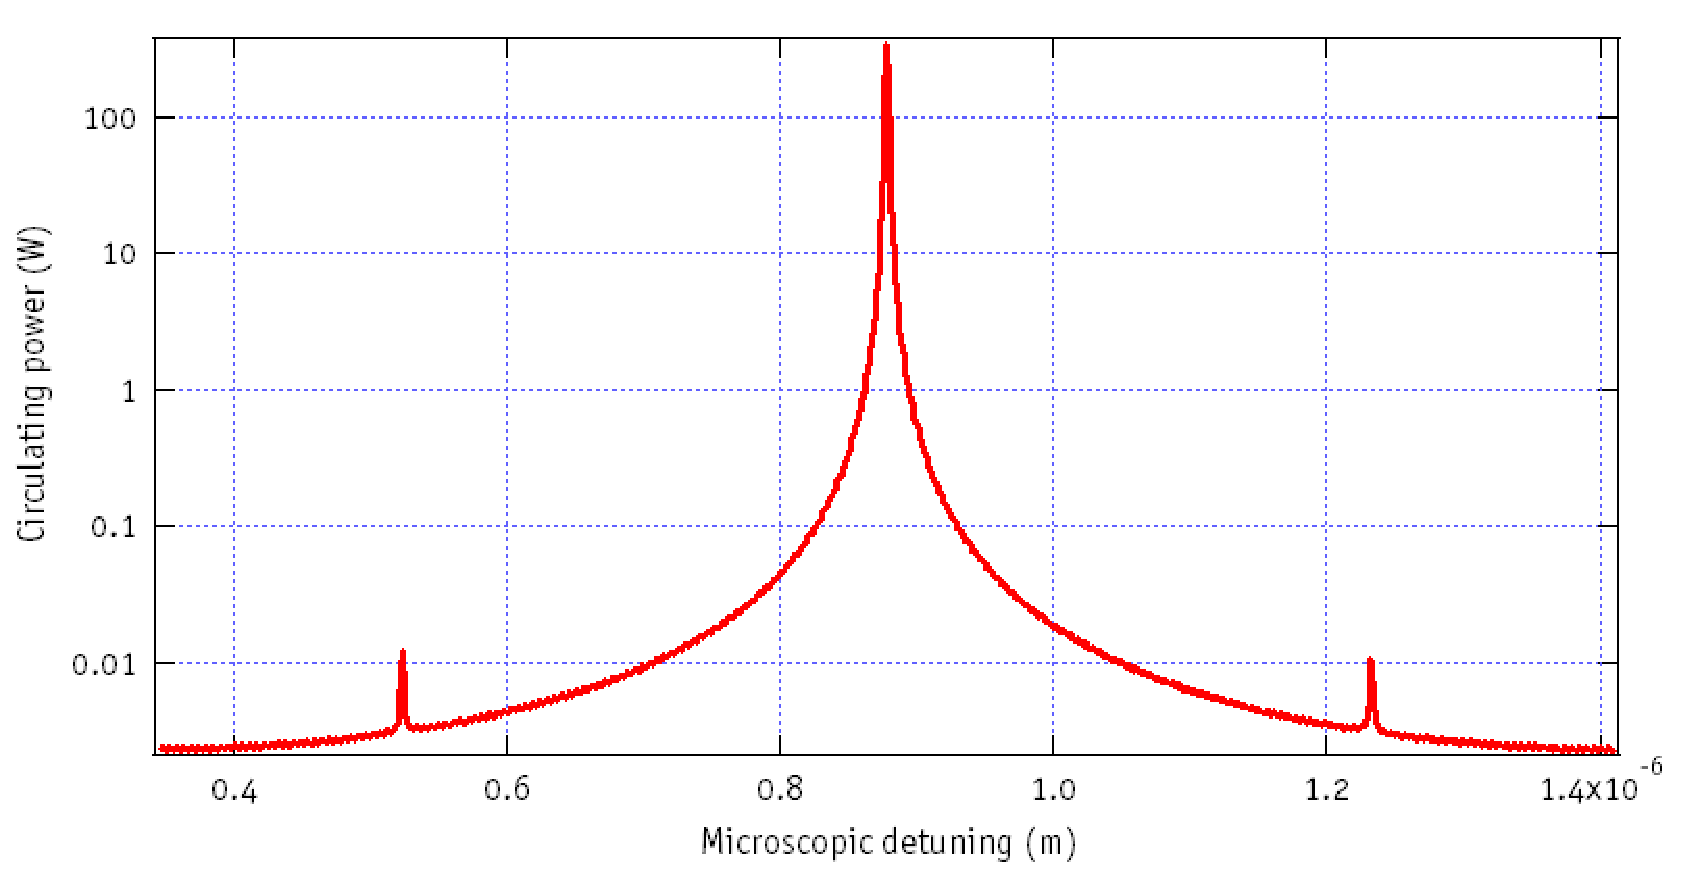
\includegraphics[width = 0.9\textwidth]{Fig3_PDH_Pcirc.pdf}
\end{center}
\caption{Circulating power inside the cavity as the cavity is scanned over one FSR. The two small peaks around the main resonance indicate the resonance of the sidebands. \label{fig3:PDH_P}}
\end{figure}

\begin{figure}
\begin{center}
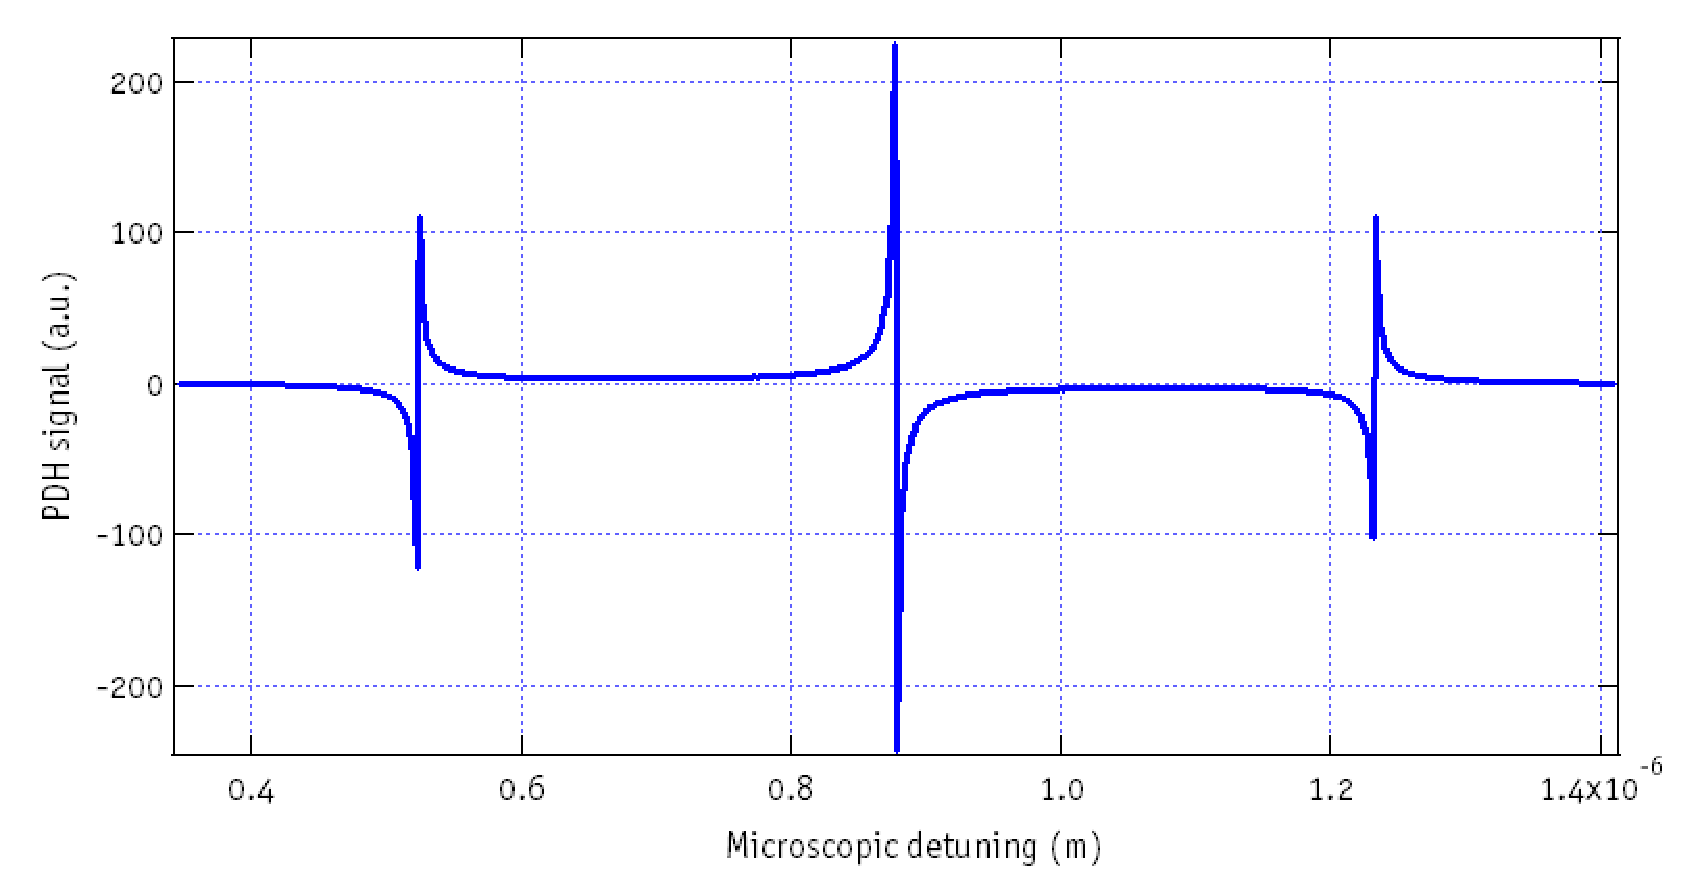
\includegraphics[width = 0.9\textwidth]{Fig3_PDH_E.pdf}
\end{center}
\caption{Pound Drever Hall error signal as a function of the detuning.\label{fig3:PDH_E}}
\end{figure}

\clearpage

\section{Simulation of a three mirrors ring cavity}
\label{cha3.5}

We can try now to add an additional mirror to our simulations and simulate a three mirrors ring cavity, often used as a mode cleaner. In the previous example we have been dealing with an optical beam perpendicular to the optical surface, this is no longer the case as seen in figure \ref{fig3:MC1}. The fact that the incident beam arrives with an angle to the surface is the main difficultly for this kind of simulation. However as we will see this problem can easily be overcome.\\

\begin{figure}
\begin{center}
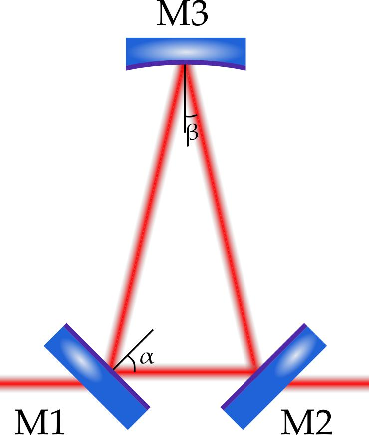
\includegraphics[width = 0.5\textwidth]{Fig3_MC.pdf}
\end{center}
\caption{Optical setup of a three mirrors ring cavity. Unlike a Fabry-Perot cavity, where the mirrors are usually perpendicular to the incident beam, for the mode cleaner the incoming beam arrives with a large angle on the two bottom mirrors. The mirror notation used in the OSCAR example are also indicated. \label{fig3:MC1}}
\end{figure}

In the OSCAR mode cleaner example (folder \textcolor{blue}{Simulate\_mode\_cleaner}), we suppose that the incident plane is horizontal. We keep this convention in the manual and it is relatively easy to adapt the code for any arbitrary angle of incidence. Let's examine what is happening on reflection: as soon as the angle of incidence of an electric field to a reflective surface is different from zero, two effects can arise:
\begin{itemize}
  \item The reflected beam will present astigmatism directly related to the angle of incidence.
  That can be understood by imagining that the incident beam will be stretched in the horizontal direction as it is projected to the mirror surface upon reflection.
  \item The beam on reflection will get flipped in the horizontal direction, this is purely a geometrical effect and the reader can easily be convinced by looking at the figure \ref{fig3:MC_flip}.
\end{itemize}

\begin{figure}
\begin{center}
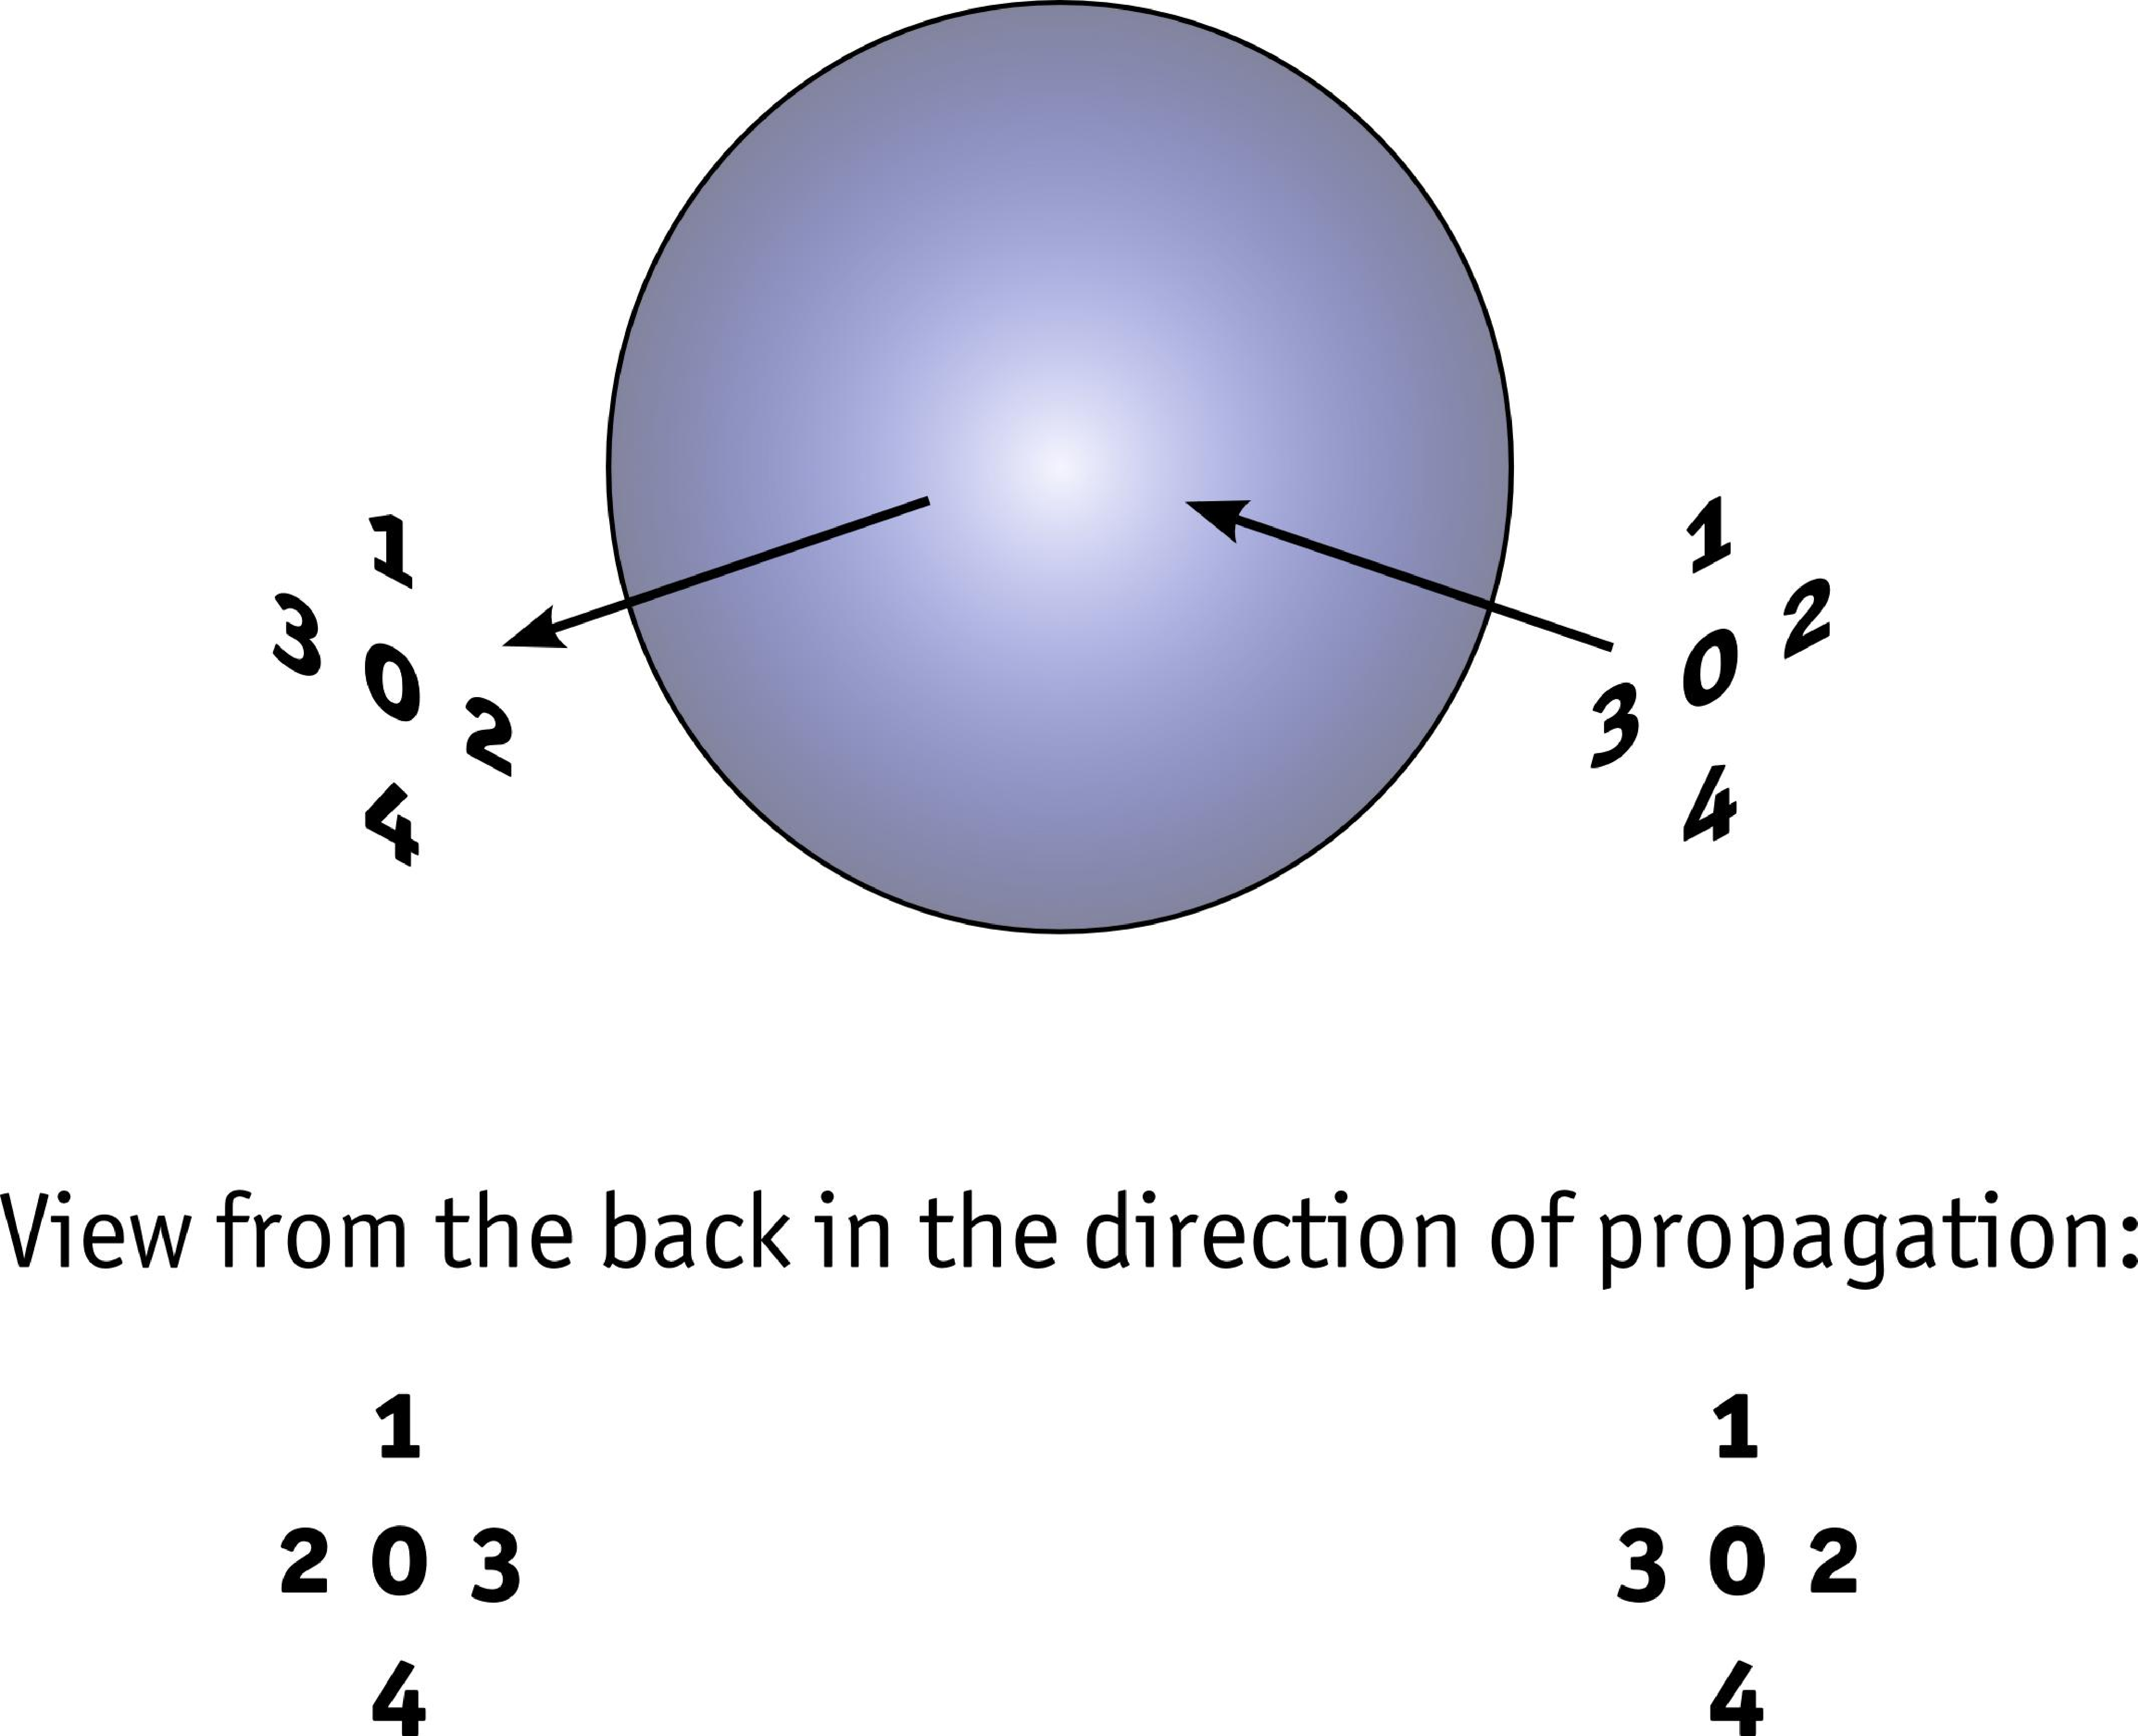
\includegraphics[width = 0.5\textwidth]{Fig3_MC_flip.pdf}
\end{center}
\caption{Example of an image reflected by a mirror. It is interesting to see that after reflection the image is flipped in the horizontal direction. \label{fig3:MC_flip}}
\end{figure}

The two items described above are implemented in OSCAR in the new function \emph{Propa\_mirror} showed in the listing \ref{lis3:mc}. Compared to the function \emph{Propa\_mirror} seen in the first chapter (section \ref{sec1:3:5}), we have added one new input parameter: \textsl{Grid\_angle\_X}. \textsl{Grid\_angle\_X} is a new distorted 2D grid representing the projection of the grid used for propagation (called \textsl{Grid.D2}) to the mirror surface.

\begin{lstlisting}[float=btp,caption=Reflection on a mirror for arbitrary angle of incidence\label{lis3:mc},frame=lines]
% Stretch the laser beam as seen by the mirror
Output = Propa_mirror(Wave_field, Wave_mirror, reflec,Grid_angle_X)

Output = interp2(Grid_angle_X,Grid.Y,Wave_field,Grid.X,Grid.Y,'cubic');

Output = Output .* exp(-i * Wave_mirror*Laser.k_prop) * reflec .* Mirror.mask;


% Go back to the normal grid
Output = interp2(Grid.X,Grid.Y,Output,Grid_angle_X,Grid.Y,'cubic',0);

% Flip the matrix along the x axis
Output = Output(:,Grid.Num_point:-1:1);
\end{lstlisting}

The function used to simulate the reflection on a mirror can be decomposed in the following steps:
\begin{enumerate}
  \item Project the incident beam on the mirror surface. So the incident beam will look astigmatic.
  \item Reflect the projected incident beam in the same way as a incoming beam normal to the mirror surface
  \item Project the reflected beam to the on the plane of propagation
  \item Flip the beam in the horizontal plane
\end{enumerate}

The steps described above are directly implemented in Matlab as shown in the script \ref{lis3:mc}.

In the examples provided with OSCAR, the transmission of a 3 mirrors ring cavity is presented. To show the mode cleaning effect, the input beam is the normalised sum of the TEM$_{10}$ and TEM$_{01}$. As expected both modes have different resonance condition inside the mode cleaner as shown in figure \ref{fig3:MC_reso}. The microscopic resonance length of the two modes is separated by half a wavelength, which is the expected result since the mode TEM$_{10}$ encountered an extra $3\pi$ shift during its round trip propagation.


\begin{figure}
\begin{center}
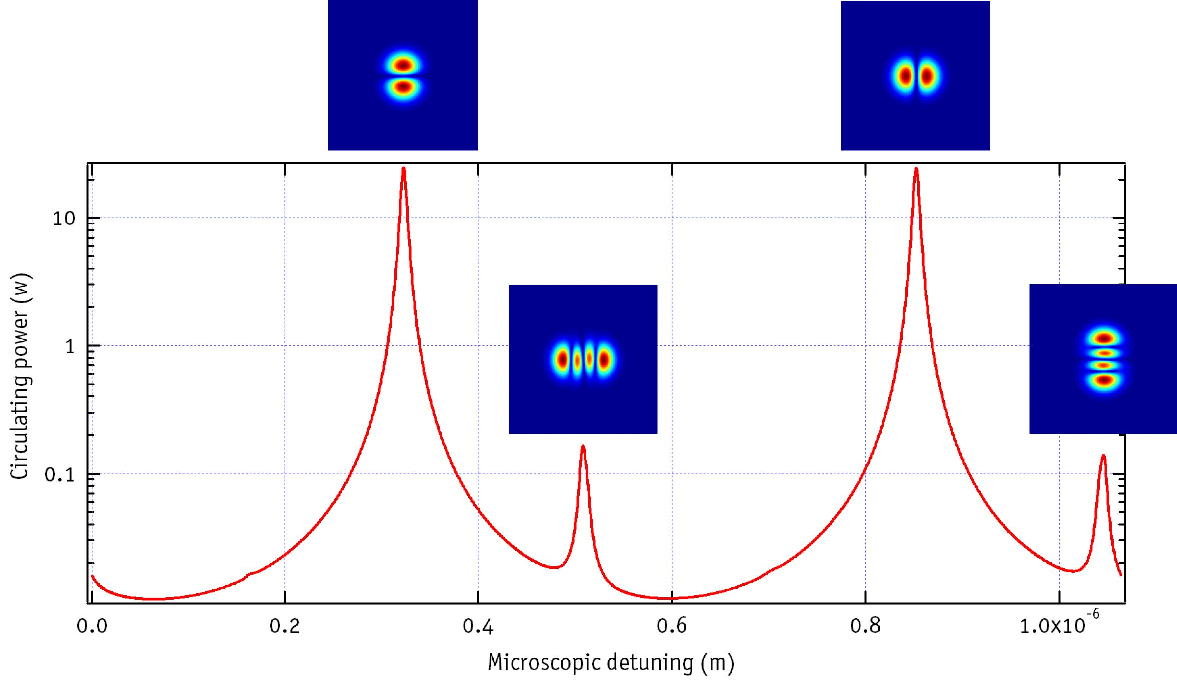
\includegraphics[width = 0.8\textwidth]{Fig3_MC_reso.pdf}
\end{center}
\caption{Scan of the mode cleaner over one free spectral range. The two main peaks are due to the resonance of the TEM$_{01}$ and TEM$_{10}$. Additional peaks in the spectrum indicates a slight modemismatching. \label{fig3:MC_reso}}
\end{figure}


For this example, we set the working point of the cavity for the mode TEM$_{10}$ to be resonant inside the cavity. The transmitted field from the mode cleaner is shown at the bottom right corner of figure \ref{fig3:MC_res}. As we would hope the transmitted field is a pure TEM$_{10}$. For consistency, we also check that the reflected field is very similar to a pure TEM$_{01}$, but not exactly since the input beam was not perfectly matched to the cavity.

\begin{figure}
\begin{center}
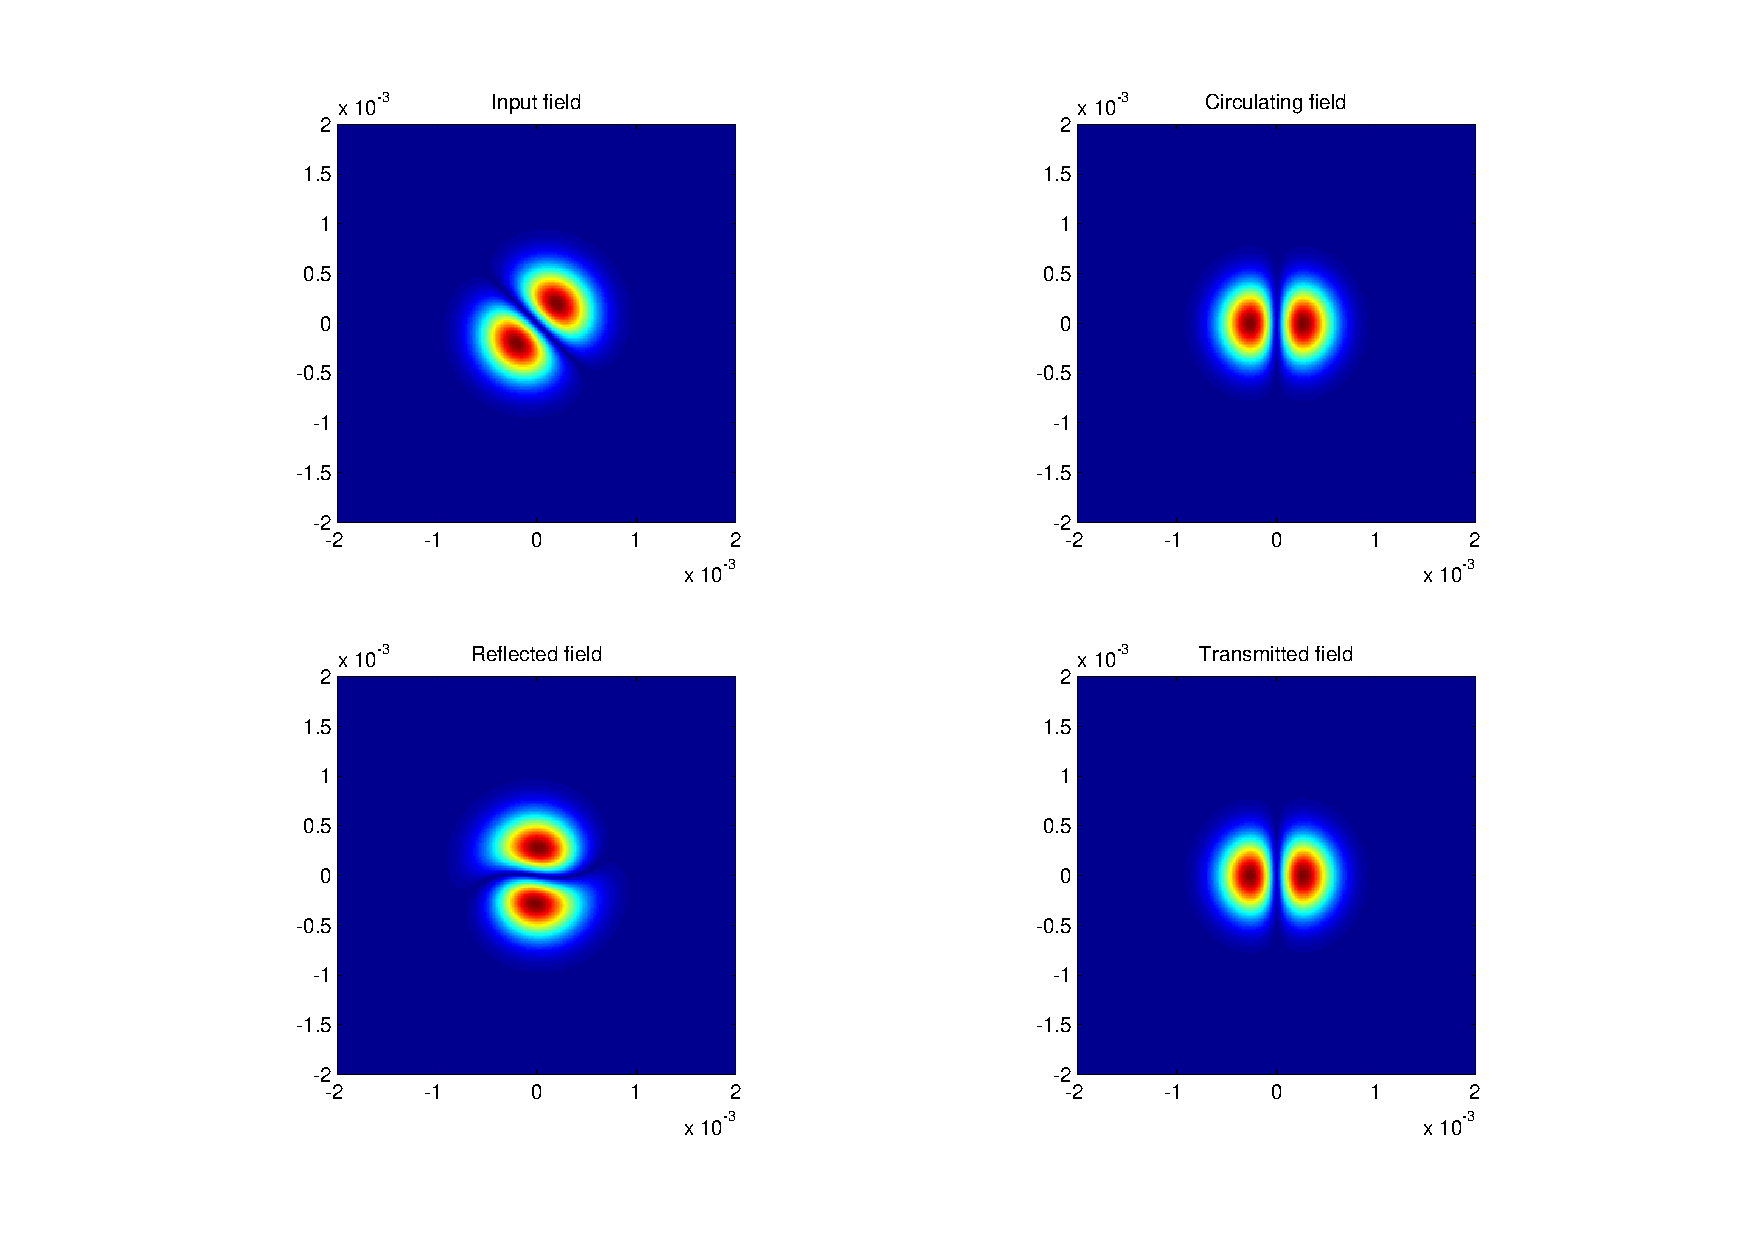
\includegraphics[width = 1.0\textwidth]{Fig3_MC_res2.pdf}
\end{center}
\caption{Output screen from OSCAR. The input field, a sum of TEM$_{10}$ and TEM$_{01}$ is shown on the top left corner. The reflected and the transmitted field are shown respectively in the bottom left and right picture.  \label{fig3:MC_res}}
\end{figure}

Below is the output from OSCAR:

\begin{verbatim}
 ------ Display the results ------
 Circulating power (W): 49.524735
 Reflected power (W): 0.503506
 Transmitted power (W): 0.495243
\end{verbatim}

So the mode cleaner was able to separate the mode TEM$_{10}$ and TEM$_{01}$. We have slightly more power reflected than transmitted by the cavity, this is a direct consequence of the fact that the input beam is not perfectly matched to the cavity.

\begin{verbatim}
 ---- Display results for cavity C1 -----
 Round trip diffraction loss: 35.6127 [ppm]
 Circulating power: 49.8224 [W]
 Size of the beam on the end mirror: 0.0205821 [m]
 Size of the beam on the input mirror: 0.020576 [m]
 Size of the cavity waist: 0.0183982 [m]
 Distance of the cavity waist from the input mirror: -500.471 [m]
\end{verbatim}




\part{OSCAR V3: the Oriented Object version}

%\textcolor{blue}{My\_First\_FFT\_code.m}
%\chapter{Version 3.0: some big changes}


\chapter{The big changes}

For this new version of OSCAR the code has been totally rewritten using the Oriented Object capability of Matlab. The code is now more user friendly and less prone to errors. Moreover some new functions has been added and the higher order optical modes are supported from the start.

The principle of the FFT code and the method to derive results are still unchanged, so for people not familiar with FFT code, it is strongly recommended to read the first part of this manual.

\paragraph{Requirements} The new OSCAR works with Matlab version superior to 2009a and the \textsl{Optimization Toolbox} is necessary if beam fitting functions are used.

\section{Motivation and goals}

 First, the curious reader may wonder why there is no version 2.0 of OSCAR. Such a version exists, it is OSCAR classic with the implementation of a power recycled Michelson with Fabry Perot arm cavities. This version was developed to simulated LIGO-Virgo type of interferometers but was never officially distributed.

 The code of version 2.0 was becoming messy since OSCAR was not intended to be so advanced (remember, it was only supposed to simulate the test cavity at Gingin in Australia). To include all the code developed for the version 2.0, it was decided to write a full new version of OSCAR taking also into account all what I learned as a OSCAR user.

 Doing a new version allowed some radical changes: no more global variables, add change of refractive index, sidebands field managed automatically at the same time as the carrier, manage higher order modes and much more\dots In the long term OSCAR should be able to simulate Advanced gravitational wave detectors with realistic optics and that in a very simple script.

 The new code should also take into account the computing progress made in recent years. For example, the version 3.0 has been written with parallel processing in mind, for example the North and West arms could be computed in parallel on different cores of the CPU (the Parallel Processing Toolbox is then required) or a cavity scan can use up to 8 cores. Calculations on the GPU will also be integrated (when I get suitable computer).

 The new code can also use separate grid size in the same simulation. That could be used to simulate non degenerated recycling cavities, where the laser beam has to be strongly focused and could change size by a factor 10.

\section{The new objects and how to use them}

The main change of this version for the user is the use of Oriented Object programming for OSCAR. A laser field or a mirror are no longer complex 2D matrices but are objects with different attributes. Each object is part of a class, for example the laser beam is an instance of the class \textsl{E\_field}, a mirror surface is an object from the class \textsl{Interface}. Functions are defined to work on specific class and not on any random 2D data.

The definition of the classes and their associated functions are presented in the following subsections. In the description of the function call, argument and output variables in \textbf{bold} are mandatory. For more detailed descriptions of the functions and the associated syntax, the help of Matlab can be used (help followed by the name of the function).

\subsection{The class Grid}
\textbf{G1} = \textcolor{blue}{Grid}(Nb\_points\_grid,Size\_grid)
by default: Nb\_points\_grid~=~256 and Size\_grid~=~1 \\

The class \textsl{Grid} is used to represent the discretisation of the space and all the associated variables (see \ref{App3:grid} for the details). It was formerly known as the global variable \textsl{Grid} in OSCAR classic. One \textsl{Grid} object is the first object to be defined in a OSCAR script. To define an instance of the class \textsl{Grid}, 2 parameters are necessary: the number of pixels used (typically 128 or 256) and the size of the grid in meter. For example:

\begin{verbatim}
G1 = Grid(128,0.40);
\end{verbatim}

Define the object \textsl{G1} of the class \textsl{Grid}, then later all the objects for the simulations will be defined on a grid of $128 \times 128$ with a side length of 40~cm.

Only one function is associated with the class \textsl{Grid}, it is \textcolor{blue}{What\_is\_possible}. \textcolor{blue}{What\_is\_possible}(\textbf{G1}) returns for the grid \textsl{G1} what is the maximum curvature or tilt for a mirror of diameter \textsl{diam}. By default the mirror diameter is 80\% of the size of the grid and the wavelength is set to 1064~nm.

It is is possible to change manually the diameter of the mirror and the wavelength of the laser by using the optional arguments \emph{'diam'} and \emph{'wavelength'}: \verb? What_is_possible(G1,'diam',0.2,'wavelength',633E-9) ?

\noindent \textbf{map2D} = \textcolor{blue}{Do\_Virtual\_map}(\textbf{G}, \textbf{Power\_law})
\vspace*{-0.2cm}
\begin{quote}
Function to create a synthetic map from a given PSD. The PSD is parameterized as a (or several) power law. The function return a 2D height map of the surface which can then after be applied to a Interface object. See the example \textcolor{blue}{Example\_Display\_Create\_maps.m} for a practical implementation.
\end{quote}


\subsection{The class E\_field}
\textbf{E1} = \textcolor{blue}{E\_field}( \textbf{Grid\_name} , \emph{options}) by default the laser beam is in the fundamental mode

Instances of the class \textsl{E\_field} are laser beams, represented as electric field in a complex 2D matrix. The objects \textsl{E\_field} contain a wavelength (1064 nm by default) and also the refractive index of the medium where the laser beam is. If sidebands are present, they are also implemented in the object at the same time as the carrier. All the variables and parameters of objects \textsl{E\_field} are detailed in \ref{App3:E_field}.

Since OSCAR version 3.05, there is now different ways to define a laser beam:
\begin{itemize}
  \item with the waist: \\
        \verb? E_input = E_Field(G1,'w0',0.02) ?
  \item with the waist and a distance: \\
        \verb? E_input = E_Field(G1,'w0',0.02,'z',-10) ?
  \item with a beam radius and a wavefront curvature: \\
        \verb? E_input = E_Field(G1,'w',0.018,'R',-1420) ?
  \item with the complex q parameter: \\
        \verb? E_input = E_Field(G1,'q',12 + 1200*1i) ?
  \item the optical mode can also be specified, for example for a helicoidal mode LG 3 3:
        \verb? E_input = E_Field(G1,'w0',0.02,'mode','LG_HELI 3 3') ?
        To define the mode basis, 3 options are possible: 'HG n m', 'LG\_HELI n m' or 'LG\_SIN n m'
\end{itemize}
A non distributed function exist also to create astigmatic beam. Most of OSCAR's functions are applied to objects of this class. The essential functions are described below:\\

\noindent \textbf{E2} = \textcolor{blue}{Add\_HOM}(\textbf{E1}, \textbf{max\_mode\_order})
\vspace*{-0.2cm}
\begin{quote}
Add some higher order optical modes to a fundamental mode. It is possible to choose the power distribution of the higher order modes.
\end{quote}

\noindent \textbf{E2} = \textcolor{blue}{Add\_sidebands}(\textbf{E1}, \textbf{mod freq}, \textbf{mod index})
\vspace*{-0.2cm}
\begin{quote}
Create two frequency shifted sidebands fields from a carrier E\_Field \textsl{E1} as the phase modulator would do in the optic lab. The separation frequency between the carrier and the sideband is given by \textsl{mod freq}, and the modulation index by \textsl{mod index}. At present in OSCAR, no sidebands of sidebands is allowed.
\end{quote}

\noindent overlap = \textcolor{blue}{Calculate\_Overlap}(\textbf{E1,E2})
\vspace*{-0.2cm}
\begin{quote}
Calculate the overlap integral between 2 E\_field. The function returns the complex normalised overlap between the 2 fields. Without any output argument, the function returns in the command window the power coupling (i.e. square of the absolute value of the overlap integral) between the field E1 and E2.
\end{quote}

\noindent overlap = \textcolor{blue}{Calculate\_Overlap\_SB\_Car}(\textbf{E1})
\vspace*{-0.2cm}
\begin{quote}
Calculate the overlap integral between the carrier and the lower and upper sidebands for one E\_field. The function returns two complex normalised numbers which are the overlap between the carrier and the two sidebands. Without any output argument, the function returns in the command window the power coupling (i.e. square of the absolute value of the overlap integral).
\end{quote}

\noindent power = \textcolor{blue}{Calculate\_power}(\textbf{E1},'include','carrier'|'all'|'SB')
\vspace*{-0.2cm}
\begin{quote}
Calculate the total power of the E\_Field \textsl{E1}. The function can either return a number or display the value in the Matlab command line if no output variable is used. A similar function \textcolor{blue}{Calculate\_power\_SB} exists to calculate the power of the sidebands fields.
To simulate a DC photodiode, which will sum all the field frequencies, one can use  \textcolor{blue}{Calculate\_power}(E1,'include','all').
\end{quote}

\noindent \textbf{E2} = \textcolor{blue}{Change\_E\_n}(\textbf{E1},\textbf{n})
\vspace*{-0.2cm}
\begin{quote}
Change the refractive index where the laser beam is. Could be use to pass through a flat interface from a vacuum to a mirror substrate for example.
\end{quote}

\noindent return\_param = \textcolor{blue}{Check\_pos\_tilt}(\textbf{E1})
\vspace*{-0.2cm}
\begin{quote}
Use as a diagnostic tool to check the centroid position of the beam on the grid as well as its tilt, function in both directions at the same time.
\end{quote}

\noindent [\textbf{sig\_p sig\_q}] = \textcolor{blue}{Demodulate\_SB}(\textbf{E1})
\vspace*{-0.2cm}
\begin{quote}
Demodulate the field \textsl{E1} with the present pair of sidebands. As the result, the in phase \textsl{sig\_p} and in quadrature \textsl{sig\_q} signals are given. This function could be used to derive a Pound Drever Hall error signal as shown in \ref{ch4:ex_PDH}.
\end{quote}

\noindent Mat\_scattered = \textcolor{blue}{Expand\_HOM}(\textbf{E1},\textbf{max\_mode\_order})
\vspace*{-0.2cm}
\begin{quote}
Expand the beam \textsl{E1} into the Hermitte Gauss basis defined by \textsl{E1} (\textsl{E1} must be close to a fundamental mode). The result is given as the normalised power content in the different optical modes. If not output is given a plot is made. Several options are possible:
\end{quote}
\begin{itemize}
  \item to output all the power content into the different higher order modes up to the order 10 \\
        \verb? Expand_HOM(E1,10,'display','pyramid') ?
  \item to define a different basis for the calculation given as beam radius and complex wavefront curvature in meter\\
        \verb? Expand_HOM(E1,10,'basis',[0.05 -1400]) ?
\end{itemize}


\noindent \textcolor{blue}{E\_plot}(\textbf{E1})
\vspace*{-0.2cm}
\begin{quote}
Display a 2D plot of the field amplitude in a new Matlab figure window. Function can also be used as \textsl{E1}.E\_plot(). We can also display the amplitude in log scale \verb?E_plot(E1,'space','log')? or the propagating angle of the beam \verb?E_plot(E1,'angle')?. To create illustrative picture of the beam without all the axis, one can use the option \verb?'no_axis',true?.

A similar function exist also for the sidebands (but with less options): \noindent \textcolor{blue}{E\_plot\_SB}
\end{quote}


\noindent [beam\_radius wavefront\_RofC] = \textcolor{blue}{Fit\_E\_Field}(\textbf{E1})
\vspace*{-0.2cm}
\begin{quote}
This function is used to find the beam parameter of the field \textsl{E1}, it can also be used for higher order modes. If no output are given the result is written in the Matlab command window. To fit only the fundamental mode, it is faster to use the function \textcolor{blue}{Fit\_TEM00}.

For the fit of an astigmatic fundamental mode, it is recommended to use the function \textcolor{blue}{Fit\_TEM00\_xy}.
\end{quote}


\noindent [\textbf{Eout},\textbf{Gout}] = \textcolor{blue}{Focus\_beam\_with\_telescope}(\textbf{Ein},\textbf{array\_L\_D})
\vspace*{-0.2cm}
\begin{quote}
With this function, one can now simulate mirrors with small radius of curvature to simulate strongly focused beam. The method has been inspired by the work done J.Y. Vinet \cite{Virgo_PB} and H. Yamamoto \cite{Hiro1}.
The new function can dynamically adapt the size of the grid and as such the focused beam is defined on a new grid. This function is used to simulate the focusing mode matching telescope at the input or output of the interferometer.
The input argument is the input field and a vector with the focal length of the equivalent mirror/lens and the separation between the optical elements in meters. A telescope with several lenses can be simulated with only one call of the function.
See the provided example for more details.
It has also the possibility to add maps and finite size optics to the telescope.
\end{quote}

\noindent \textbf{E2} = \textcolor{blue}{Normalise\_E}(\textbf{E1},power)
\vspace*{-0.2cm}
\begin{quote}
Normalise the E\_field \textsl{E1} to 1~W if no \textsl{power} argument is specified. Only the carrier is affected by this function and not the sidebands.
\end{quote}

\noindent \textbf{E2} = \textcolor{blue}{Propagate\_E}(\textbf{E1},\textbf{dist})
\vspace*{-0.2cm}
\begin{quote}
Propagate the field \textsl{E1} over a distance \textsl{dist} in meter. If sidebands are present, the sidebands are automatically propagated at the same time, with of course the adequate phase shift.
\end{quote}

\noindent \textbf{E2} = \textcolor{blue}{Reflect\_mirror}(\textbf{E1},\textbf{I1})
\vspace*{-0.2cm}
\begin{quote}
Returns the field after reflection on a mirror. \textsl{I1} is an Interface object which must have been previously defined. An alternative syntax could be \textcolor{blue}{Reflect\_mirror}(\textbf{E1},\textbf{R1}), with \textsl{R1} the radius of curvature of the mirror to be reflected on. A concave mirror is represented by a positive \textbf{R1}.

Reflections inside the substrates are allowed since the index of refraction is taken into account for the reflection.
\end{quote}


\noindent E3 = \textcolor{blue}{ Remove\_00\_part}(\textbf{E1},E2)
\vspace*{-0.2cm}
\begin{quote}
Remove the fundamental Gaussian part from a field \textbf{E1}. That is useful to see which higher order modes are superposed with the fundamental mode following some cavities simulations. Can also be used to subtract 2 fields E1 and E2 as in the case of destructive interferences.
\end{quote}


\noindent \textbf{E2} = \textcolor{blue}{Transmit\_Aperture}(\textbf{E1},\textbf{size}, 'circle' $\mid$ 'square')
\vspace*{-0.2cm}
\begin{quote}
Transmit the field \textsl{E1} through an aperture of diameter \textsl{size}. The aperture could be round or square, if not specified it is round. Custom aperture can also be defined see the function help for example.
\end{quote}

\noindent \textbf{E2} = \textcolor{blue}{Transmit\_lens}(\textbf{E1},\textbf{focal length})
\vspace*{-0.2cm}
\begin{quote}
Transmit the field \textsl{E1} through a lens of a given focal length.
\end{quote}

\noindent [\textbf{E\_trans} E\_ref]= \textcolor{blue}{Transmit\_Reflect\_Interface}(\textbf{E1},\textbf{I1})
\vspace*{-0.2cm}
\begin{quote}
Transmit and reflect the field \textsl{E1} through an interface \textsl{I1}. The orientation of the interface is given by the refractive index of the incoming field \textsl{E1}.
\end{quote}

For convenience, the operators +,- and * have also been overloaded to work with any object \textsl{E\_field}.

\subsection{The class Prop\_operator}
\label{Sec:DI}
This is an internal class which must be almost invisible for the user. The objects of this class allows to speed up the propagation of electrical field \textsl{E\_Field} thanks to the pre-calculation of the propagation matrix. A \textsl{Prop\_operator} is automatically created when a cavity is created. It represents the propagation operator over one cavity length.

Since OSCAR 3.10, a new method of propagation has been implemented based on the method of digital integration \cite{DI_paper}. This method is slower, however it eliminates the light leaking out from the simulation grid. With the direct implementation, a minimal distance of propagation is essential for the validity of this technique. The distance depends on the size of the grid and can be checked with the function \textcolor{blue}{What\_is\_possible}.

To enable the digital integration, one has to set the logical variable \textsl{Prop\_operator.Use\_DI} to true. For example, to use the digital integration for the simulation of the cavity \textsl{C1}, we will write:

\verb? C1.Propagation_mat.Use_DI = true; ?

The parameters included in the class \textsl{Prop\_operator} are described in \ref{App3:Prop_OP}\\


The creator for this class is:

\noindent \textbf{Prop} = \textcolor{blue}{Prop\_operator}(\textbf{Grid\_name},\textbf{Length}, n)

\vspace*{-0.2cm}
\begin{quote}
The variable \textsl{Length} represents the propagation length in meter. One can also specify an optional parameter \textsl{n}, the refractive index of the media, that way, thick substrate can also be implemented.
\end{quote}
To propagate a laser beam (and its sidebands) one can simply use:

\verb?  E2 = Propagate_E(E1, Prop) ?

\subsection{The class Interface}
\textbf{I1} = \textcolor{blue}{Interface}(\textbf{Grid\_name},options)

The class \textsl{Interface} is used to represent a surface which separates two media of refractive index. Objects of this class are used to represent mirrors, lenses or curved interfaces between air and glass. The structure of the class \textsl{Interface} is described in \ref{App3:Inter}.

To define a concave mirror for a laser beam, the radius of curvature must be positive. Internally in OSCAR, the sagitta of the surface view from the medium n1 toward n2 will be negative by convention. The surface is stored in the variable \textsl{I1.surface}.

Below are some ways to define an interface:
\begin{itemize}
  \item Interface to define a curved surface of radius 1000~m between the refractive 1 and 1.45 \\
        \verb?  Interface(Grid,'RoC',1E3,'n1',1,'n2',1.45) ?
  \item a mirror with an aperture of 20~cm of diameter \\
      \verb?  Interface(Grid,'RoC',1E3,'CA',0.2) ?
   \item a mirror with an aperture of 20~cm of diameter and angle of incidence of 3 degrees \\
      \verb?  Interface(Grid,'RoC',1E3,'CA',0.2,'AoI',3) ?
  \item add the transmission of 1\% and loss of 50 ppm\\
        \verb?  Interface(Grid,'RoC',1E3,'CA',0.2.'T',0.01,'L',50E-6) ?
\end{itemize}
The options can be defined in any order. To define flat mirrors, a \verb?'RoC'? of \verb?0 or Inf? can be used. Check the file \verb?@Interface/Interface.m? to see the default parameters.

The list of methods associated with the objects of the class \textsl{Interface} is given below:

\noindent \textbf{I2} = \textcolor{blue}{Add\_astigmatism}(\textbf{I1}, \textbf{Zernike amplitude}, \textbf{Diameter})
\vspace*{-0.2cm}
\begin{quote}
Add to the surface of the interface \textsl{I1} the Zernike polynomial 2,2 (which represents the astigmatism) with an amplitude of \textsl{Zernike amplitude} and over a diameter \textsl{Diameter}.
\end{quote}


\noindent \textbf{I2} = \textcolor{blue}{Add\_map}(\textbf{I1}, \textbf{filename}, options)
\vspace*{-0.2cm}
\begin{quote}
Add to the surface of the interface \textsl{I1} a square map loaded from the file \textsl{filename}. For square maps, the resolution of one pixel must be given by the parameters \verb?'reso'?. The map can also be normalised to a certain RMS using the option \verb?'RMS'? or the height can be scaled by scalar with the option \verb?'scale'?. One can also rotate the map by a number of time 90 degrees with the option \verb?'rotate'?. The option \verb?'remove the tilt and focus'? can remove the tilt focus from the added map. The tilt/focus is removed over all the surface but with the optimal calculated only over a diameter.

Here some examples:
\begin{itemize}
  \item load the file map1.dat \\
        \verb? I1 = Add_map(I1,'map1.dat','reso',3.5E-4) ?
  \item load the map and scale it to 1 nm RMS \\
        \verb? I1 = Add_map(I1,'map1.dat','reso',3.5E-4,'RMS',1E-9) ?
  \item rotate the map by 90 degree \\
        \verb? I1 = Add_map(I1,'map1.dat','reso',3.5E-4,'rotate',1) ?
  \item remove the tilt and focus \\
         \verb? I1 = Add_map(I1,'map1.dat','reso',3.5E-4,'remove_tilt_focus',0.150) ?
\end{itemize}

Maps with cylindrical symmetry can be loaded as a 2 columns text file. First column is the radius and the second is the height in meter. In that case the resolution does not have to be specified. To supress the output, the option \verb?'verbose',false? can be used. A new experimental argument is \verb?'centering'? to offset the map if this region of interest is not at the center.
\end{quote}


\noindent \textbf{I2} = \textcolor{blue}{Add\_tilt}(\textbf{I1}, \textbf{tilt\_angle}, 'x')
\vspace*{-0.2cm}
\begin{quote}
Tilt the whole surface of the interface \textsl{I1} by the amount \textsl{tilt\_angle} in radian. It is possible to specify the direction of the tilt by setting the third argument \textsl{'x'} or \textsl{'y'}. By default the tilt is in the vertical direction (recommended solution).
\end{quote}


\noindent \textbf{I2} = \textcolor{blue}{Cut\_frequency\_Interface}(\textbf{I1},\textbf{Option},\textbf{f\_cut})
\vspace*{-0.2cm}
\begin{quote}
Remove given spatial frequency within a given interface object. The argument \textsl{Option} is a string \verb?'LP'?, \verb?'HP'? or \verb?'BP'? for respectively low pass, high pass or band pass filter. \textsl{f\_cut} is the cutting spatial frequency in m$^{-1}$, for band pass filtering \textsl{f\_cut} is vector of two frequencies.\\
The implementation for the filtering is done in a straight forward manner (see the simple code), so as a result artefact may appear in the resulting object \textsl{I2}.
\end{quote}


\noindent I2 = \textcolor{blue}{Expand\_Zernike}(\textbf{I1},options)
\vspace*{-0.2cm}
\begin{quote}
Expand in Zernike polynomials the interface \textsl{I1}. Two options are available: 'Z\_order', an integer which represents the maximum order of the Zernike polynomials to take in to account in the calculations and 'diam', the diameter where the Zernike polynomials are defined. This function returns the interface \textsl{I2}, which is the interface reconstructed by the Zernike polynomials. Example:
\verb? I2 = Expand_Zernike(I1,'Z_order',10,'diam',0.2) ?
\end{quote}


\noindent \textcolor{blue}{I\_plot}(\textbf{I1})
\vspace*{-0.2cm}
\begin{quote}
Plot the surface of the interface \textsl{I1}. The color scale is in meter. \verb? I_plot(I1,'diam',0.160)? will only plot the surface over a diameter of 160mm.
\end{quote}


\noindent \noindent [\textbf{PSD\_1D} \textbf{freq}] = \textcolor{blue}{Plot\_PSD}(\textbf{I1}, options)
\vspace*{-0.2cm}
\begin{quote}
Function used to calculate the one dimension Power Spectral Density (PSD) of a surface. The two output arguments are the vector of the PSD and the vector of the frequency. By default before calculating the PSD 2D, a Hanning window is applied to the data and the PSD is calculated summing all the frequencies over one direction to pass from 2D to 1D. A detailed explanation of the different ways to calculate the PSD can be found in a Hiro LIGO note \cite{Hiro_PSD}.

An example for the possible options can be found below, combination of the different options is allowed:
\begin{itemize}
  \item Calculate the PSD over a given diameter, given in meter \\
        \verb? [PSD_1 freq] = Plot_PSD(I1,'diam',0.150) ?
  \item Calculate the PSD by summing radial frequencies \\
        \verb? [PSD_1 freq] = Plot_PSD(I1,'rect_1D',false) ?
  \item Use a Gaussian weighting to calculate the PSD, must input the Gaussian beam radius (in meter) \\
        \verb? [PSD_1 freq] = Plot_PSD(I1,'window_Gaussian',0.05) ?
  \item Plot directly the PSD in the current window \\
        \verb? [PSD_1 freq] = Plot_PSD(I1,'display',true) ?
\end{itemize}
\end{quote}


\noindent RMS = \textcolor{blue}{Weighted\_RMS}(\textbf{I1,Ein})
\vspace*{-0.2cm}
\begin{quote}
Calculate the RMS of the surface \textsl{I1} weighted by the intensity of the field \textsl{Ein}. A diameter can also be given as the second argument. Beware the curvature is not subtracted before the calculation, so a perfectly curved spherical mirror will have a non zero RMS.
\begin{itemize}
  \item Calculate the weighted RoC \\
        \verb? RMS = Weighted_RMS(I1,E_Field(G1,'w',0.05)) ?
  \item Display directly the calculated RMS \\
        \verb? Weighted_RMS(I1,0.2) ?
\end{itemize}
\end{quote}


\noindent RoC\_fitted = \textcolor{blue}{Weighted\_RoC}(\textbf{I1,Ein})
\vspace*{-0.2cm}
\begin{quote}
Calculate the radius of curvature of the surface \textsl{I1} weighted by the intensity of the field \textsl{Ein}. This calculation is useful to fit non perfectly spherical surface. A diameter can also be given as the second argument.
\begin{itemize}
  \item Calculate the weighted RoC \\
        \verb? RoC = Weighted_RoC(I1,E_Field(G1,'w',0.05)) ?
  \item Display directly the radius of curvature \\
        \verb? Weighted_RoC(I1,0.2) ?
\end{itemize}
\end{quote}

The operators \verb?+?,\verb?-? have also been overloaded to be used with object of the class \textit{Interface}.

\subsection{The class Mirror}
\textbf{M} = \textcolor{blue}{Mirror}( \textbf{I\_HR}, \textbf{I\_AR}, \textbf{Substrate\_length})

This class can simulate thick substrates. The substrate can be part of a cavity as an input mirror for example. If the substrate is part of the cavity, the surface \textsl{I\_HR} is supposed to be the HR coating (and hence inside the cavity).

\textsl{I\_HR} and \textsl{I\_AR} are 2 objects of the class \textsl{Interface}. The 2 interfaces must share the same refractive index superior to 1. \textsl{Substrate\_length} is a scalar used to represent the thickness of the substrate in meter.

The mirror object can also be used to simulate the etalon effect. Indeed if the AR surface is imperfect (R\_AR $>$ 0), light can be bounced several times within the substrate before exiting. The number of round trip is hard-coded but can be changed using the line (by default it is 1):

 \verb? M.RT_inside=3 ?

Two similar procedures can be used with the class \textsl{Mirror}. The procedures simulate the transmission and reflection of an E\_field by an instance of the class \textsl{Mirror}:

\noindent [\textbf{E\_trans} E\_ref]= \textcolor{blue}{Transmit\_Reflect\_Mirror}(\textbf{E1},\textbf{M1},'AR')
\vspace*{-0.2cm}
\begin{quote}
Calculate the transmitted and reflected fields (\textsl{E\_trans} and \textsl{E\_ref} respectively) by an object \textsl{M1} of the class Mirror. The input beam is \textsl{E1}. The first interface to consider, indicating the direction of the incoming beam can be either the HR or AR surfaces according to the last argument 'HR' or 'AR' .
\end{quote}

A new function \textcolor{blue}{Transmit\_Reflect\_Optic} has also been created which can be used by either Interface object or Mirror object. Internally, this function calls the function \textcolor{blue}{Transmit\_Reflect\_Interface} or \textcolor{blue}{Transmit\_Reflect\_Mirror} depending on the input parameters.

\subsection{The class Cavity1}
\textbf{C1} = \textcolor{blue}{Cavity1}( \textbf{I1}, \textbf{I2}, \textbf{Cavity\_length}, \textbf{E1})

This class is used to simulate Fabry Perot cavities. Objects of the class \textsl{Cavity1} are cavities constituted by two Interface objects \textsl{I1, I2} separated by a distance \textsl{Cavity\_length}. An input field \textsl{E1} must also be given. \textsl{I1} is considered as the input surface where the input beam is defined, whereas \textsl{I2} is the end mirror.

The input field can be defined either inside the cavity on the surface \textsl{I1} or outside the cavity. In the later case, the input beam will first be transmitted through \textsl{I1} which can act as a lens. By default the input beam is defined inside the cavity, if it is not the case the user can add in his script:
\begin{verbatim}
C1.Laser_start_on_input = false ;
\end{verbatim}

Variables of instances of the class \textsl{Cavity1} are listed in {App3:Cavity}.

\noindent Several functions are associated with the class \textsl{Cavity1}:

\noindent \textbf{Cout} = \textcolor{blue}{Calculate\_fields}(\textbf{Cin})
\vspace*{-0.2cm}
\begin{quote}
\textcolor{blue}{Calculate\_fields} calculates the fields on resonance inside the cavity and stored them for future use. Compared to \textcolor{blue}{Get\_info} this function also calculates the reflected field, so the input laser beam has can not be defined inside the cavity. The results can be displayed using \textcolor{blue}{Display\_results}(Cout).
Before the finding the steady state fields inside the cavity, the cavity working point (i.e the resonance condition) has to be set, for example using the function \textcolor{blue}{Cavity\_resonance\_phase}.
With the option argument \verb?'iter'? or \verb?'accuracy'?, one can set the level of accuracy (and hence the computational time) for the simulation.
\end{quote}

\noindent \textbf{Cout} = \textcolor{blue}{Calculate\_fields\_AC}(\textbf{Cin})
\vspace*{-0.2cm}
\begin{quote}
\textcolor{blue}{Calculate\_fields\_AC} is similar to the function \textcolor{blue}{Calculate\_fields} except it used the accelerated convergence scheme \cite{Saha:97,DAY_AC} to find the steady state fields inside the cavity. The gain in speed could be important if the cavity is close to a perfect cavity, so the steady field is near a perfect fundamental mode.
This function works for the carrier and for the sideband fields, if present. Also for a better convergence it is recommended to use the digital integration method for the propagation of the field (see \ref{Sec:DI}).
A second function \textcolor{blue}{Calculate\_fields\_AC2} using another more advanced convergence scheme which can give more accurate results.
\end{quote}

\noindent \textbf{Cout} = \textcolor{blue}{Calculate\_RT\_mat}(\textbf{Cin})
\vspace*{-0.2cm}
\begin{quote}
Calculate the round trip kernel of the cavity for the electrical field. This is later use to calculate the cavity eigenmodes and eigen values. The kernel itself is a 2D complex matrix of size \textsl{Nb\_points}$^2$ $\times$ \textsl{Nb\_points}$^2$, so the kernel can real take out a lot of memory. On a desktop, one might want to limit textsl{Nb\_points} to 64, while on a powerful desktop one can go up to 128.

To calculate the kernel, the digital integration technique has to be used for the beam propagation. This technique to be valid required a minimum propagation distance which depends on the size of the grid. If this is a problem, the kernel can be calculated on a different grid (contact the author for more details on this topic).
\end{quote}

\noindent \textbf{Cout} = \textcolor{blue}{Cavity\_lock\_PDH}(\textbf{Cin})
\vspace*{-0.2cm}
\begin{quote}
Adjust the resonance condition to minimise the error signal derived from a Pound Drever Hall locking scheme \cite{black:79}. To calculate the error signal a pair of sidebands must be present and the function \textcolor{blue}{Cavity\_resonance\_phase} must first be run.
\end{quote}

\noindent \textcolor{blue}{Check\_stability}(\textbf{Cin})
\vspace*{-0.2cm}
\begin{quote}
Calculate the radius of curvature of the input and end mirrors and then check the stability and gain of the cavity. Function useful when mirror maps with curvature are used. An optional second argument could be given to specify the diameter on which the mirror radius of curvature is calculated. For example to calculate the stability of the cavity only taking into account the central 6 cm diameter of the mirror, one can use:
\verb? Check_stability(C1,'diam',0.06) ?
The function also return the input beam parameters of the fundamental mode for a perfect mode matching.

\end{quote}

\noindent \textcolor{blue}{Check\_matching}(\textbf{Cin},nb\_RT)
\vspace*{-0.2cm}
\begin{quote}
Propagate the input beam back and forth between the cavity input and end mirrors and check the beam size before each reflection. The mode matching is good if during multiple round trips the beam size on the mirror does not fluctuate (but could be different of course on the input and end mirror). The optional argument \textsl{nb\_RT} can set the number of round trip to be done.
\end{quote}

\noindent \textbf{Cout} = \textcolor{blue}{Cavity\_resonance\_phase}(\textbf{Cin})
\vspace*{-0.2cm}
\begin{quote}
Calculate the macroscopic length tuning to bring the cavity on resonance for the input field. The cavity resonance has to be found before any calculations on the cavity (circulating fields, loss calculations,\dots) are launched. The input and output arguments are usually the same.
A second function \textcolor{blue}{Cavity\_resonance\_phase2} is also present, this function gives more accurate results when the cavity is degenerated.
\end{quote}

\noindent \textbf{Cout} = \textcolor{blue}{Cavity\_scan}(\textbf{Cin})
\vspace*{-0.2cm}
\begin{quote}
Scan the cavity over one free spectral range and then set the cavity resonance to maximise the circulating power. This procedure is much slower than \textcolor{blue}{Cavity\_resonance\_phase} but can still be useful to check if some higher order modes are excited since after the FSR scan can be displayed.
The presence of sidebands in the input beam of the cavity can also be implemented. First the sidebands have to be defined and then the option \verb? 'With_SB',true? must be added in the command.
\end{quote}

\noindent \textcolor{blue}{Display\_cavity\_modes}(\textbf{Cin},'N',10,'Airy',1)
\vspace*{-0.2cm}
\begin{quote}
Display the cavity eigen modes. The function \textcolor{blue}{Calculate\_RT\_mat} must first has been run, so the cavity kernel has been calculated. With this function one can display an arbitrary number of modes (by default the first 20) and also draw the Airy peak of the cavity with the command:

  \verb? Display\_cavity\_modes(C1,'N',30,'Airy',1) ?

An example of how to use the function \textcolor{blue}{Display\_cavity\_modes} is shown in the script \textcolor{blue}{Example\_cavity\_eigenmodes.m}
\end{quote}

\noindent \textcolor{blue}{Display\_scan}(\textbf{Cin})
\vspace*{-0.2cm}
\begin{quote}
Display the scan from a cavity after the procedure \textcolor{blue}{Cavity\_scan} was run. By moving the cursor on the upper plot (circulating power vs tuning), the profile of the optical modes can be checked in the lower right plot.
\end{quote}

\noindent \textcolor{blue}{Get\_info}(\textbf{Cin})
\vspace*{-0.2cm}
\begin{quote}
\textcolor{blue}{Get\_info} calculates the fields on resonance inside the cavity. The function is also use to calculate the diffraction loss due to the mirror finite size.
\end{quote}



\subsection{The class CavityN}

\textbf{CN} = \textcolor{blue}{CavityN}( \textbf{I}, \textbf{D}, \textbf{E1})

This class introduces linear cavity with arbitrary number of mirrors. \textsl{I} represents a vector of object Interfaces, \textsl{D} is a vector of distances and finally \textsl{E1} is the input laser field.

Two kinds of cavity could be defined:
\begin{itemize}
  \item A ring cavity where the laser beam is reflected on each mirror only once during one round trip (3 or 4 mirrors mode cleaner cavity falls in this category). In that case, the length of the vector \textsl{I} is the same as the one of \textsl{D}.
  \item A folded cavity, where during one round trip the laser beam is reflected twice by the intermediate mirrors (think recycling folded cavity of LIGO). In that case, it has one more interface \textsl{I} than length \textsl{D}.
\end{itemize}


The distance  \verb|D(n)| is defined as the distance between the interfaces  \verb|I(n)| and  \verb|I(n+1)|. The functions suitable for the class \textsl{CavityN} are the same as for the class \textsl{Cavity1} without exception.

An example of how to use the class \textsl{CavityN} is shown in the script \textcolor{blue}{Example\_4mirrors.m}

\subsection{The class Mirror}

This class is used to simulate optics with thick substrates. So a mirror is defined as 2 surfaces separated by a distance with a certain refractive index. Typically, one surface is coated with an anti-reflective coating while the second surface has a high reflectivity coating.

Similar to a cavity, the light can do several round trip within the substrate if the anti-reflection is not perfect. So the Mirror object can be used to simulate the etalon effect within a substrate. It is not possible to set the resonance condition in the substrate but one can scan the substrate length over wavelength to check this effect.

Mirror object can be used with the class \textsl{Cavity1} to form a cavity between the 2 high reflectivity surfaces.


\section{What to expect in the following versions}

Most of the code for the release V3.0 was frozen in September 2012. Some additional functions have already been implemented and are little by little moving in the official distribution. The motor behind most the new development is the need to simulate accurately the off axis secondary beams in the Advanced Virgo marginally stable recycling cavities.

Two main new features have already been implemented but not released:

\begin{itemize}
  \item \textbf{Use of rectangular grid.} It is possible to use grid with different size and number of points in the horizontal and vertical directions. That is useful to simulate tilted beams with large angle along one direction since in that case a fine resolution is required. A special version of OSCAR in 1D has also been made but may never get released.
  \item \textbf{Simulation of a dual recycled Michelson interferometer.} A new class has been defined to simulate a dual recycled Michelson interferometer. That is done for marginally stable cavity but not yet released due to a lack of comprehensive documentation.
   \item \textbf{GPU portability.} Use of Nvidia graphic card to speed up the calculation.
\end{itemize}

If need urgently some new functions and can not wait for future versions, you can contact directly the author.

%-----------------------------------------------------------------------------------

\chapter{New examples of simulations}\label{ch4:ex}

After the formal previous chapter, here is the most interesting part: the concrete examples. In this part we will see how easy it is to create simulations with the new OSCAR, few lines of code are usually enough to get a result.

\section{Beam parameters after a thick lens}

Before learning how to define cavities, we can already see how to propagate a laser beam through a custom made thick lens. The lens is bi-convex, made of fused silica (n=1.45) and is 4\,cm thick . The first surface has a radius of 1\,km and the second 2\,km. At the exit of the lens, we propagate the beam further by 200\,m and then measure its parameter. The commented script is called \textcolor{blue}{Example\_Thick\_lens.m} and can be found in the OSCAR folder.\\

The first surface is defined in OSCAR by the line:

\noindent \verb|L1 = Interface(G1,-1000,0.10,1,0,1,1.45)|. Since the surface is convex as seen from the incoming laser beam there is a minus sign. The second argument is the clear aperture of the optic, then there are the transmission and the loss (in power) and finally the two refractive index of the media on either part of the interface.

To transmit the laser beam \verb|E1| through the interface, the command is simply \verb|E2 = Transmit_Reflect_Interface(E1,L1)|. Then the beam is propagated along 4\,cm with the command \verb|E2 = Propagate_E(E2,0.04)| and finally passes through the second interface.

At the end of the script, the laser beam parameter are displayed using the command \verb|Fit_TEM00(E3)|. The condensed script for the transmission of the thick lens is shown in the listing \ref{lis4:ex_Thick_lens}.\\

\begin{lstlisting}[float=htp,caption=Example of OSCAR script to simulate a thick lens\label{lis4:ex_Thick_lens},frame=lines]
G1 = Grid(256,0.3);
E1 = E_Field(G1,0.02);

L1 = Interface(G1,-1000,0.10,1,0,1,1.45);
L2 = Interface(G1,2000,0.10,1,0,1.45,1);

E2 = Transmit_Reflect_Interface(E1,L1);
E2 = Propagate_E(E2,0.04);
E2 = Transmit_Reflect_Interface(E2,L2);

E3 = Propagate_E(E2,200);
Fit_TEM00(E3);
\end{lstlisting}

At the end, the beam radius is measured to be 1.76283\,cm and the wavefront curvature -1765.36\,m. To be compared with the result found using the ABCD matrix for the same setup: Beam radius of 1.76283\,cm and wavefront curvature of -1763.79\,m. So both results are in good agreement.

Since OSCAR 3.10, the thick lens can be made with an instance of the class Mirror. This example has been updated accordingly.

\section{Calculating diffraction loss and circulating power}

In this example, we will calculate the circulating power in a Fabry Perot cavity. At the same time, we can also derive the diffraction loss due to the finite size of the mirrors.

The Fabry Perot cavity is 1\,km long and the input and end mirrors have a radius of curvature of 2500~\,m. Both mirrors have a transmission of 2\% and no loss. The diameter of the mirror is set to 10~cm. The incident beam has a beam radius of 2\,cm and a radius wavefront curvature of 2500\,m.\\

The 7 lines of the script to define and the cavity and do the calculations can be found in the listing \ref{lis4:cav_circ}. This script with additional commented lines can be found in the OSCAR3.0 folder under the name \textcolor{blue}{Example\_Pcirc.m}.

\begin{lstlisting}[float=htp,caption=Example of OSCAR script to calculate the circulating power\label{lis4:cav_circ},frame=lines]
G1 = Grid(128,0.3);
E_input = E_Field(G1,0.02,-2500);

IM = Interface(G1,2500,0.10,0.02,0);
EM = Interface(G1,2500,0.10,0.02,0);

C1 = Cavity1(IM,EM,1000,E_input);
C1 = Cavity_resonance_phase(C1);
Get_info(C1);
\end{lstlisting}

The script takes less than 10s to run on a modern laptop. At the end, \emph{Get\_info(C1)} returns a detailed list of information regarding the cavity with a plot of the circulating power and the power buildup. Return of \emph{Get\_info(C1)} in the Matlab command line:

\newpage

\begin{verbatim}
 ---- Display results for cavity C1 -----
 Round trip diffraction loss: 35.6127 [ppm]
 Circulating power: 49.8224 [W]
 Size of the beam on the end mirror: 0.0205821 [m]
 Size of the beam on the input mirror: 0.020576 [m]
 Size of the cavity waist: 0.0183982 [m]
 Distance of the cavity waist from the input mirror: -500.471 [m]
\end{verbatim}

To speed up the calculation of the steady state field, it is possible to use the function \emph{C1 = Calculate\_fields\_AC(C1)} in conjunction with \emph{C1.Display\_Results}.

\section{Scan of a misaligned cavity}

Using the same cavity parameters as in the previous example, we will now tilt the end mirror in the vertical direction by 1~microradian. To see the excitation of higher optical modes, we will display the circulating power over one free spectral range. The script for that simulation is presented in the listing \ref{lis4:cav_scan}.

\begin{lstlisting}[float=htp,caption=Example of OSCAR script to scan a cavity \label{lis4:cav_scan},frame=lines]
G1 = Grid(128,0.3);
E_input = E_Field(G1,0.02,-2500);

IM = Interface(G1,2500,0.10,0.02,0);
EM = Interface(G1,2500,0.10,0.02,0);
EM = Add_tilt(EM,1E-6,'y');

C1 = Cavity1(IM,EM,1000,E_input);
C1 =  Cavity_scan(C1);
Display_scan(C1);
\end{lstlisting}

The script takes around 2 minutes to run. The output is the Matlab figure shown in the figure \ref{fig4:scan}. The top plot is a cavity scan over one free spectral range. We can notice 3 peaks, from left to right the first peak is a LG$_{10}$ due to imperfect mode matching, the second is the mode HG$_{10}$ and the third one, the highest is the fundamental mode.

\begin{figure}
\begin{center}
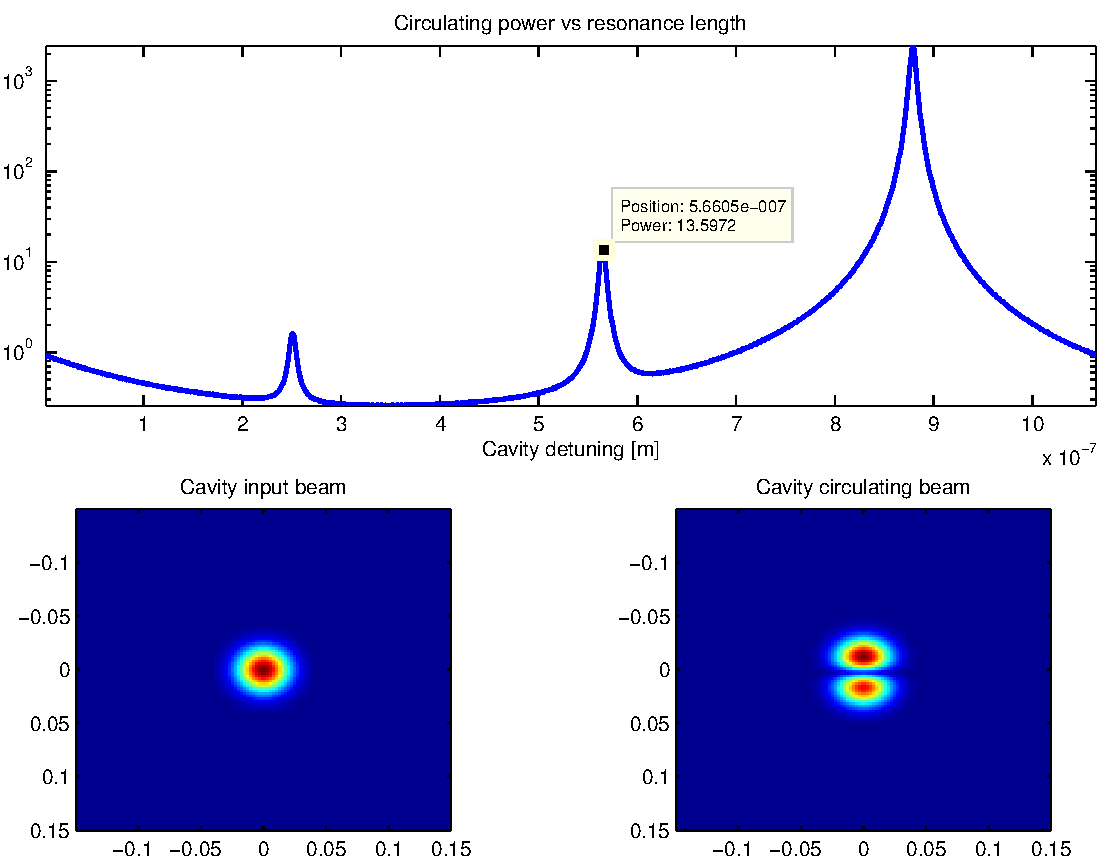
\includegraphics[width = 0.99\textwidth]{Fig5_scan.pdf}
\end{center}
\caption{\label{fig4:scan} Output window of the function \emph{Display\_scan(C1)} with the cavity scan over one FSR on top.}
\end{figure}

\section{Mirror maps and higher order modes}

In this example, we will demonstrate how to use higher order optical modes in conjunction with mirror maps. The mirror maps are stored in text files under the form of a matrix which represents the mirror height fluctuations in meter. In the maps given, the mirror curvature is not included (but it could be done). The RMS of the mirror maps is around 2~nm, typical of very good large mirrors.

The laser beam is now defined outside the cavity, so the cavity reflected field can also be calculated. The script for this example is called \textcolor{blue}{Example\_HOM\_with\_maps.m} and is shown in the listing \ref{lis4:cav_HOM} without any comments.\\

\begin{lstlisting}[float=htp,caption=Example of OSCAR script to calculate the reflected field from a cavity with maps \label{lis4:cav_HOM},frame=lines]
G1 = Grid(512,0.4);
E_input = E_Field(G1,0.043,-1034,'LG',3,3);

IM = Interface(G1,1500,0.35,0.02,0);
EM = Interface(G1,1700,0.35,0.02,0);

IM = Add_map(IM,'Map1.txt',1.5E-3);
EM = Add_map(EM,'Map2.txt',1.5E-3);

C1 = Cavity1(IM,EM,3000,E_input);
C1.Laser_start_on_input = false ;

C1 = Cavity_resonance_phase(C1);

C1 = Calculate_fields(C1);
Display_results(C1);
\end{lstlisting}

The line \verb|IM = Add_map(IM,'Map1.txt',1.5E-3)| is used to add the custom 2D map to the surface \verb|IM|. The map does not have to have the same size of the grid since internally an interpolation is done. The third argument \verb|1.5E-3| is the step size of the map in meter. The map can be normalise to a certain RMS by including a fourth argument such as: \verb|IM = Add_map(IM,'Map1.txt',1.5E-3,1E-9)|. In that case the map is automatically normalise to have a RMS of 1~nm.
Regarding the sign convention, positive values in the mirror maps reduce the length of the cavity.\\

After the definition of the cavity and the calculation of the resonance length, the command \verb|C1 = Calculate_fields(C1)| is used to calculate the circulating, reflected and transmitted fields from the cavity. The fields are then stored in the instance \verb|C1| where they could be access later. To display the result graphically the command \verb|Display_results(C1)| is then used. An example of the output screen is shown in figure \ref{fig5:LG33}

\begin{figure}
\begin{center}
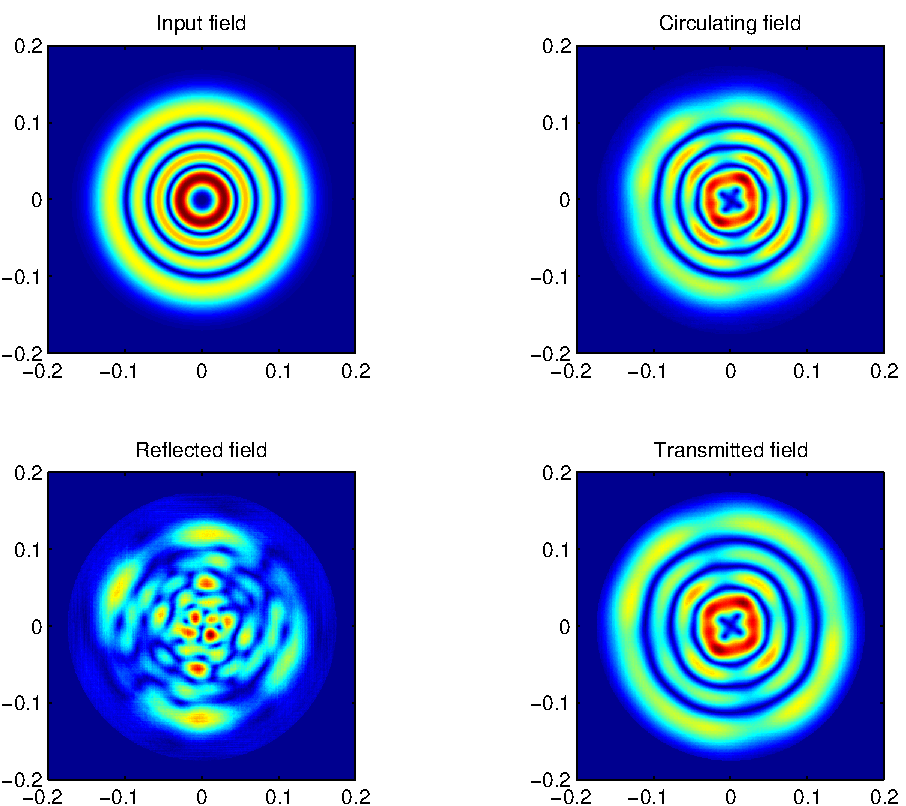
\includegraphics[width = 0.99\textwidth]{Fig5_Ref_LG.pdf}
\end{center}
\caption{\label{fig5:LG33} Output window of the function \emph{Display\_results(C1)} when a LG33 mode is expected to circulate in a cavity with realistic mirrors.}
\end{figure}

\clearpage
\section{Plotting Pound Drever Hall error signal} \label{ch4:ex_PDH}

In this example, we will learn how to create sidebands and derive a Pound Drever Hall locking signal in reflection. After the input laser \verb|E1| is defined, a virtual phase modulator creates a pair of sidebands with the command: \verb|E_input = Add_sidebands(E_input,6.7234E6,0.3)| (sideband frequency: 6.7234\,MHz and modulation depth: 0.3\,. Then the fields inside the cavity are computed for a given resonance phase.\\

To draw the PDH error signals, the reflected field from the cavity is demodulated to get the in phase and in quadrature signals. The simulation is relatively long since for the cavity scan 200 points are taken. That takes around 12 minutes on my laptop. A plot of the circulating power and the reflected PDH error signal is shown in figure \ref{fig5:PDH}.

\begin{figure}
\begin{center}
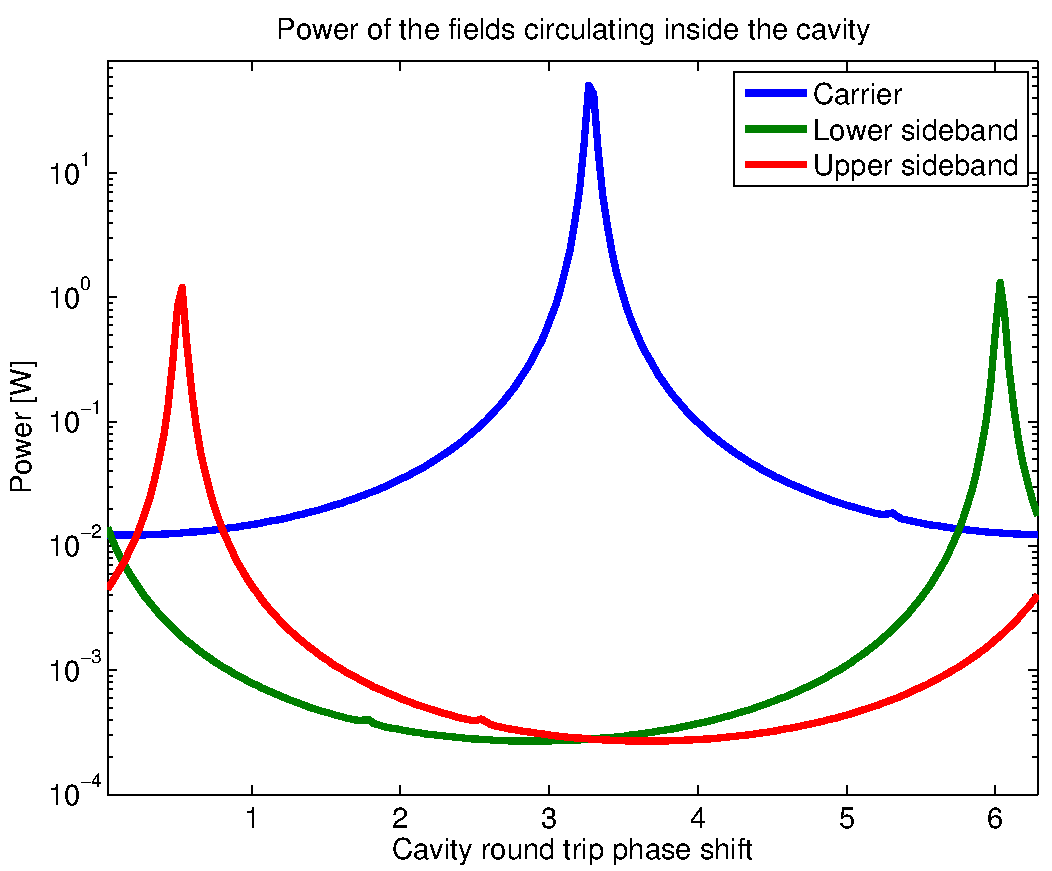
\includegraphics[width = 0.485\textwidth]{Fig5_PDH_circ.pdf}\hfill
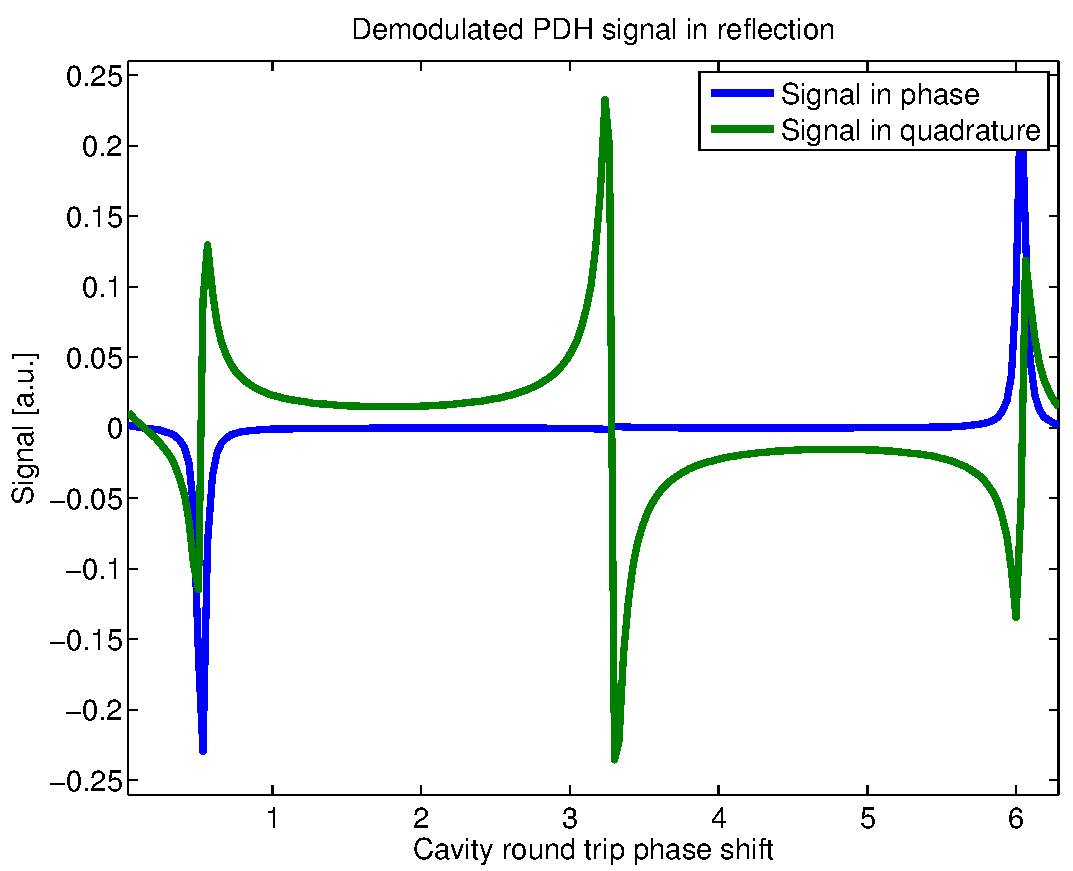
\includegraphics[width = 0.495\textwidth]{Fig5_PDH_ES.pdf}
\end{center}
\caption{\label{fig5:PDH} Circulating power inside the cavity (left) and error signals in reflection (right).}
\end{figure}

\section{4 mirrors linear cavity} \label{ch4:ex_OMC}

This example, introduces with OSCAR 3.05, shows how to simulate a 4 mirrors cavity. The parameters to define the cavity are taken from the GEO600 output mode cleaner. The script file is called \textcolor{blue}{Example\_4mirrors.m} and is rather self-explanatory for the regular user.

\section{Calculating the eigen modes of a Fabry-Perot cavity} \label{ch4:ex_OMC}

Since OSCAR V3.10, it is possible to calculate the eigens mode of a Fabry Perot or any linear cavity such as a mode cleaner. This particularly useful to check the degeneracy of a cavity or the clipping loss of higher order modes. The example file is called \textcolor{blue}{Example\_cavity\_eigenmodes.m}.

A typical display of the calculation of the cavity eigen modes is shown in figure \ref{fig5:cav_EM}.  Also, in this example file, at the end, it is shown how to display the Airy peak of the different higher order modes of the cavity.

\begin{figure}
\begin{center}
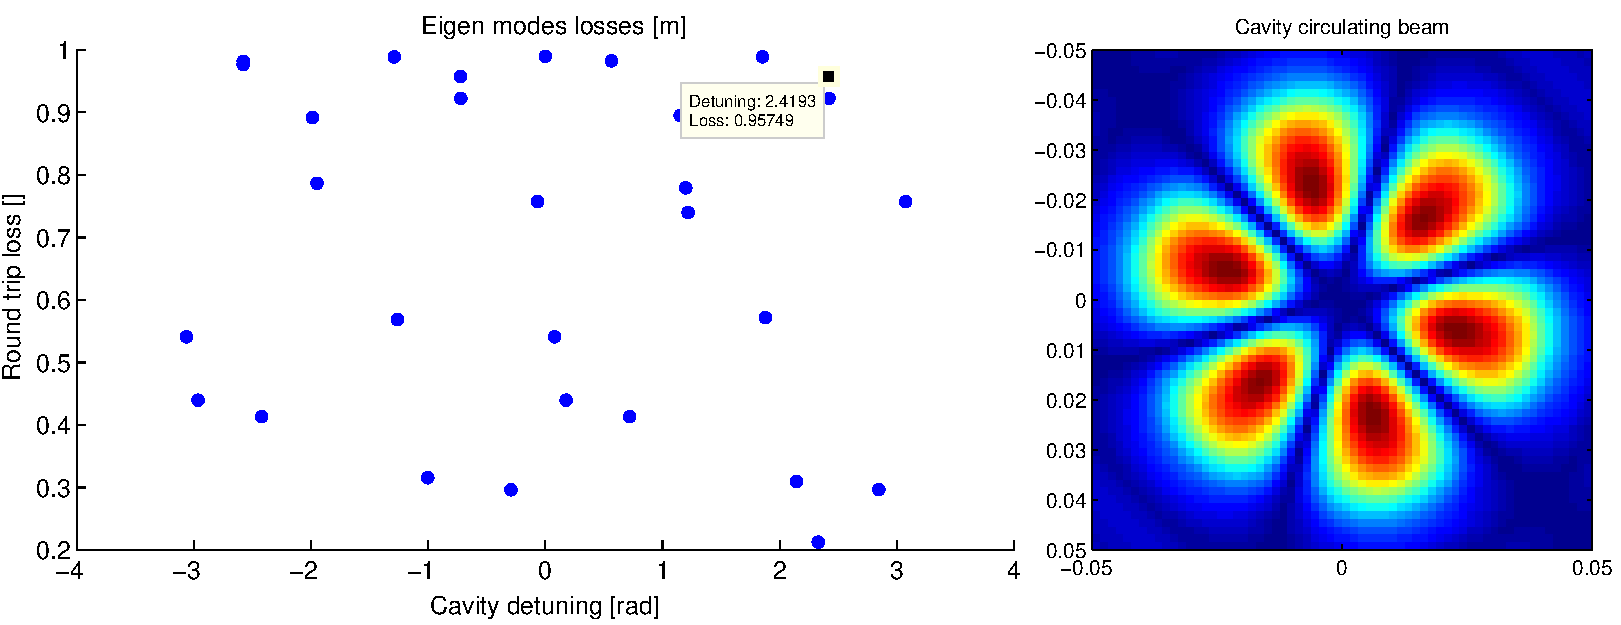
\includegraphics[width = 1.0\textwidth]{Fig5_cavity_EM.pdf}\hfill
\end{center}
\caption{\label{fig5:cav_EM} Result of the command \textcolor{blue}{Display\_cavity\_modes()}.}
\end{figure}

% FAQ
% Version 2.0 ?
% Change the accurary


%\addcontentsline{toc}{chapter}{Bibliography}
%\begin{spacing}{1}
\bibliographystyle{ieeetr}
\bibliography{biblio}
%\end{spacing}



\appendix
\part{Appendix}
\chapter{Analytical formulation of the Gaussian beam propagation using Fourier transform}

In this appendix, we will see how it is possible to rediscover all the formulas related to the laser beam propagation just by using the Fourier technique explained in chapter 1. Basically, we will do by hand the three steps which are numerically done in Matlab to propagate a Gaussian beam: first, 2D Fourier transform of the laser beam, then add the phase shift in the frequency domain and finally, inverse Fourier transform.

To facilitate the mathematical calculation, we will extensively use the following formula:

\begin{equation}
 \int^{+\infty}_{\infty} \exp \left( -ax^2 +ibx \right) dx = \sqrt{\frac{\pi}{a}} \exp \left( \frac{-b^2}{4a} \right)
\label{A1:easy}
\end{equation}


Let's consider a Gaussian beam $E(x,y,z)$ of amplitude $A$. For simplification we suppose the waist $w_0$ of the beam to be located at $z = 0$. The beam can be written:

\begin{equation}
    E(x,y,0) = A \exp\left(-\frac{x^2+y^2}{w_0^2}\right)
\end{equation}

We will now propagate the Gaussian beam along the $z$ axis over a distance $d$. To not complicate the calculation, we will just consider one transverse dimension at first, for example the dimension along $x$ since all the following equations can be decoupled in the $x/y$ dimension.

So the first step is to calculate the Fourier transform $\widetilde{E}(\nu_x,0)$ of the field $E(x,0)$:

\begin{equation}
    \widetilde{E}(\nu_x,0) = \int^{+\infty}_{\infty} A \exp\left(-\frac{x^2}{w_0^2}\right) \exp(j2\pi \nu_x x) dx
\end{equation}

Using the formula \ref{A1:easy}, the above equation becomes:

\begin{equation}
    \widetilde{E}(\nu_x,0) = A \sqrt{\pi w_0^2} \exp\left(-(\pi \nu_x w_0)^2 \right)
\end{equation}

To simulate the propagation the electric field over a distance $d$, the proper phase shift is added to Fourrier transform:

\begin{equation}
    \widetilde{E}(\nu_x,d) = A \sqrt{\pi w_0^2} \exp\left(-(\pi \nu_x w_0)^2 \right) \exp(-jkd +j \lambda \pi \nu_x^2 d)
\label{A1:4}
\end{equation}

Finally, we take the inverse Fourier transform of the equation \ref{A1:4} to go back to the familiar x space coordinate system:

\begin{equation}
\begin{split}
   E(x,d) & = \int^{+\infty}_{\infty} A \sqrt{\pi w_0^2} \exp\left(-(\pi \nu_x w_0)^2 \right) \exp(-jkd +j \lambda \pi \nu_x^2 d) \exp(-j 2 \pi \nu_x x) d \nu_x  \\
   & = A \sqrt{\pi w_0^2} \exp(-jkd) \int^{+\infty}_{\infty} \exp \left( -(\pi^2 w_0^2 - j \lambda \pi d)\nu_x^2 -j 2 \pi x  \nu_x  \right) d \nu_x \\
   & = A  \sqrt{\pi w_0^2} \sqrt{\frac{\pi}{\pi^2 w_0^2 - j \pi \lambda d}}\exp(-jkd) \exp \left(\frac{-4 \pi^2 x^2}{4 (\pi^2 w_0^2 - j \lambda \pi d )} \right)\\
   & = A \sqrt{\frac{1}{1 - j \frac{\lambda d}{\pi w_0^2}}} \exp(-jkd) \exp\left(-\frac{x^2}{w_0^2 \left(1 -j \frac{\lambda d}{\pi w_0^2}\right)}\right)
\label{A1:6}
\end{split}
\end{equation}

We can now define the usual Raleigh range $z_r$ as:

\begin{equation}
    z_r = \frac{\pi w_0^2}{\lambda}
\label{A1:7}
\end{equation}

By inserting the Raleigh range $z_r$ into \ref{A1:6} and by adding the similar result from the other $y$ transverse dimension, we obtain:

\begin{equation}
   E(x,y,d) = A \frac{1}{1 - j \frac{d}{z_r}} \exp(-jkd) \exp\left(- \frac{x^2 +  y^2}{w_0^2 \left(\frac{1}{1 - j \frac{d}{z_r}} \right) } \right)\\
\label{A1:8}
\end{equation}

Let's analyze now the two main constituent of equation \ref{A1:8}, the exponential and the complex factor in front of it. The complex number in the exponential can be separated between its real and imaginary parts:

\begin{equation}
\begin{split}
\exp\left(- \frac{x^2 +  y^2}{w_0^2 \left(\frac{1}{1 - j \frac{d}{z_r}} \right) } \right) & = \exp \left(-\frac{x^2+y^2}{w_0^2\left(1 + \frac{d^2}{z_r^2}\right)}  -j \frac{(x^2+y^2)\frac{d}{z_r}}{w_0^2\left(1 + \frac{d^2}{z_r^2}\right)} \right)  \\
& = \exp \left(-\frac{x^2+y^2}{w_0^2\left(1 + \frac{d^2}{z_r^2}\right)} -j \frac{(x^2+y^2)}{w_0^2\left(\frac{z_r}{d} + \frac{d}{z_r}\right)}              \right)  \\
& = \exp \left(-\frac{x^2+y^2}{w_0^2\left(1 + \frac{d^2}{z_r^2}\right)} -j \frac{(x^2+y^2)}{\frac{2 z_r}{k}\left(\frac{z_r}{d} + \frac{d}{z_r}\right)}              \right)  \\
& = \exp \left(-\frac{x^2+y^2}{w_0^2\left(1 + \frac{d^2}{z_r^2}\right)} -j k\frac{(x^2+y^2)}{2 d\left(1 + \frac{z_r^2}{d^2}\right)}              \right)
\end{split}
\label{A1:9}
\end{equation}

We can now consider the factor in front equation \ref{A1:8}:

\begin{equation}
A \frac{1}{1 - j \frac{d}{z_r}} = A \left(\frac{1}{1 + \frac{d^2}{z_r^2}}\right)^\frac{1}{2} \exp\left(j \arctan\left(\frac{d}{z_r} \right)\right)
\label{A1:10}
\end{equation}

Combining equations \ref{A1:9} and \ref{A1:10}, we can deduce the familiar equations governing the propagation of Gaussian beams:

\begin{equation}
   E(x,y,d) = A \frac{w_0}{w(d)} \exp\left(- \frac{x^2 +  y^2}{w(d)^2} \right) \exp \left(-j k\left(d + \frac{x^2+y^2}{2 R(d)}\right) + j \arctan\left(\frac{d}{z_r} \right) \right) \\
\label{A1:11}
\end{equation}
With:
\begin{equation}
\begin{split}
w(d) & = w_0 \left( 1 + \frac{d^2}{z_r^2}  \right)\\
R(d) & = d\left(1 + \frac{z_r^2}{d^2}\right)
\end{split}
\label{A1:234}
\end{equation}

I found remarkable that by using the simple FFT steps to propagate the beam we can rediscover all the usual equations: the normalisation factor, the evolution of the beam radius and the wavefront radius of curvature as well as the Gouy phase shift. The courageous readers can also do the calculations presented here for the higher order modes in the Hermite Gauss base.

\chapter{Finesse script}
\label{chaB}

The Finesse script \cite{Finesse} used to simulate a Fabry Perot cavity equivalent to the one described in the table \ref{tab2:param} is presented below. It is often extremely useful to create some simple Finesse model to check the exactitude of OSCAR results whenever possible. The script is also included in the OSCAR distribution under the name \textcolor{blue}{P\_circ.kat} in the folder \textcolor{blue}{Calculate\_Pcirc}.

\begin{verbatim}

l i1 1 0 n0                             # laser P=1W
gauss G1 i1 n0 0.017221 -517.112239     # Parameters for a beam radius 2cm
                                        # and a wavefront RofC of -2000m

s s0 1n 1 n0 n1
m1 SITM1 1 0 0 n1 n2
s sITM2 1n 1.45 n2 nITM
m1 ITM2 0.005 50E-6 0 nITM ncav1        # IM transmission and loss
attr ITM2 Rc -2000

s s3 1000 ncav1 ncav2

m1 ETM 50E-6 50E-6 0 ncav2 n4           # EM transmission and loss
attr ETM Rc 2000

cav cav_mode ITM2 ncav1 ETM ncav2

maxtem 8
trace 10
phase 0
startnode n0

pd0 p_circ ncav1
pd0 p_trans n4
pd0 p_ref n1

xaxis ETM phi lin -233 -234 3600
yaxis abs

gnuterm NO
retrace off

\end{verbatim}


\chapter{Details of OSCAR 3.0 classes}
The properties (i.e. parameters included in an object of a class) of the different class are described in following sections. Properties are not protected, so they can be accessed and changed using: object\_name.properties (at your own risk).

The name of the properties are usually self-explanatory and derived directly from OSCAR classic.

\section{Class Grid}

\begin{table}
  \centering
  \caption{\label{App3:grid} Details of the properties of the class \textsl{Grid} }
\begin{tabular}{|r r l|}
\hline
{\Large\strut} Properties & Type &  Comments \\
\hline
{\Large\strut} Num\_point &  scalar, integer & Should be a power of 2 \\
{\Large\strut} Length &  scalar & Length of one side of the grid (m)\\
{\Large\strut} Step &  scalar & Step = Length / Num\_point \\
{\Large\strut} Half\_num\_point &  scalar, integer & Half\_num\_point = Num\_point / 2 \\
{\Large\strut} Vector &  vector, integer & from 1 to Num\_point \\
{\Large\strut} Axis &  vector &  The scale for the grid \\
{\Large\strut} Axis\_FFT &  vector &  The spatial frequency scale\\
{\Large\strut} D2\_X &  2D matrix &  Horizontal scale in 2D \\
{\Large\strut} D2\_Y &  2D matrix &  Vertical scale in 2D \\
{\Large\strut} D2\_square &  2D matrix & Square of the distance to the center \\
{\Large\strut} D2\_r &  2D matrix & Distance from the center of the grid \\
{\Large\strut} D2\_FFT\_X &  2D matrix & Horizontal FFT scale in 2D \\
{\Large\strut} D2\_FFT\_Y &  2D matrix & Vertical FFT scale in 2D \\
\hline
\end{tabular}
\end{table}



\section{Class E\_Field}

\begin{table}
  \centering
  \caption{\label{App3:E_field} Details of the properties of the class \textsl{E\_Field} }
\begin{tabular}{|r r l|}
\hline
{\Large\strut} Properties & Type &  Comments \\
\hline
{\Large\strut} Grid &  Grid & Grid where the beam is defined \\
{\Large\strut} Field &  2D complex matrix & The carrier electric field \\
{\Large\strut} Field\_SBl &  2D complex matrix & The lower sidebands \\
{\Large\strut} Field\_SBu &  2D complex matrix & The higher sidebands \\
{\Large\strut} Refractive\_index &  scalar  & Refractive index of the medium \\
{\Large\strut} Wavelength &  scalar &  The light wavelength \\
{\Large\strut} Frequency\_Offset &  scalar &  Frequency of the sidebands \\
{\Large\strut} Mode\_name &  string &  Family and mode number \\
{\Large\strut} k\_prop &  scalar & Propagation constant \\
\hline
\end{tabular}
\end{table}

\section{Class Prop\_operator}

\begin{table}
  \centering
  \caption{\label{App3:Prop_OP} Details of the properties of the class \textsl{Prop\_operator} }
\begin{tabular}{|r r l|}
\hline
{\Large\strut} Properties & Type &  Comments \\
\hline
{\Large\strut} n &  scalar & Refractive index of the media \\
{\Large\strut} mat &  2D complex & Propagation matrix \\
{\Large\strut} dist &  scalar  & Distance of propagation \\
{\Large\strut} Use\_DI &  logical & Enable digital integration \\
{\Large\strut} mat\_DI &  2D complex  & Propagation matrix for digital integration \\
\hline
\end{tabular}
\end{table}


\section{Class Interface}

\begin{table}
  \centering
  \caption{\label{App3:Inter} Details of the properties of the class \textsl{Interface} }
\begin{tabular}{|r r l|}
\hline
{\Large\strut} Properties & Type &  Comments \\
\hline
{\Large\strut} Grid &  Grid & Grid where the beam is defined \\
{\Large\strut} surface &  2D matrix & The height of the surface \\
{\Large\strut} mask &  2D matrix of 0 and 1 & The aperture of the optic \\
{\Large\strut} T &  scalar & Transmission in power \\
{\Large\strut} L &  scalar  & Loss in power \\
{\Large\strut} n1 &  scalar &  The first refractive index \\
{\Large\strut} n2 &  scalar &  The second refractive index \\
{\Large\strut} t &  scalar &  Amplitude transmission $\sqrt{T}$ \\
{\Large\strut} r &  scalar & Amplitude reflectivity $\sqrt{1-(T+L)}$ \\
\hline
\end{tabular}
\end{table}

\section{Class Mirror}

\begin{table}
  \centering
  \caption{\label{App3:Inter} Details of the properties of the class \textsl{Mirror} }
\begin{tabular}{|r r l|}
\hline
{\Large\strut} Properties & Type &  Comments \\
\hline
{\Large\strut} I\_HR &  Interface & First surface \\
{\Large\strut} I\_AR &  Interface & Second surface \\
{\Large\strut} length\_substrate & scalar & Length of the substrate \\
{\Large\strut} RT\_inside &  integer & Number of round trip \\
{\Large\strut} n\_substrate &  scalar &  refractive index of the substrate\\
{\Large\strut} r &  scalar & Reflectivity \\
\hline
\end{tabular}
\end{table}

\section{Class Cavity1}

\begin{table}
  \centering
  \caption{\label{App3:Cavity} Details of the properties of the class \textsl{Cavity1} }
\begin{tabular}{|r r l|}
\hline
{\Large\strut} Properties & Type &  Comments \\
\hline
{\Large\strut} I\_input &  Interface & Input mirror surface \\
{\Large\strut} I\_end &  Interface & End mirror surface \\
{\Large\strut} Length &  scalar & Length of the cavity \\
{\Large\strut} Laser\_in &  E\_Field & Input laser beam \\
{\Large\strut} Laser\_start\_on\_input &  logical  & Define where the input beam is given \\
{\Large\strut} Resonance\_phase &  complex scalar &  Phase adjustment to bring the cavity on resonance \\
{\Large\strut} Cavity\_scan\_all\_field & vector of E\_Field  &  Store all the E\_field after each round trip \\
{\Large\strut} Cavity\_scan\_param &  vector &  3 values to define how to scan the cavity \\
{\Large\strut} Cavity\_phase\_param &  scalar & Number of round trip used to find the resonance \\
{\Large\strut} Cavity\_scan\_R &  vector  & Cavity circulating power scan over one FSR \\
{\Large\strut} Cavity\_scan\_RZ &  vector &  Zoom of the scan around the cavity resonance \\
{\Large\strut} Cavity\_EM\_mat &  2D complex matrix &  Cavity round trip kernel \\
{\Large\strut} Propagation\_mat & Prop\_operator & Pre-computed propagation matrix \\
{\Large\strut} Field\_circ &  E\_Field &  Cavity circulating field \\
{\Large\strut} Field\_ref &  E\_Field & Cavity reflected field  \\
{\Large\strut} Field\_trans &  E\_Field & Cavity transmitted field  \\
\hline
\end{tabular}
\end{table}

\section{Class CavityN}

\begin{table}
  \centering
  \caption{\label{App3:CavityN} Details of the properties of the class \textsl{CavityN} }
\begin{tabular}{|r r l|}
\hline
{\Large\strut} Properties & Type &  Comments \\
\hline
{\Large\strut} I\_array &  Vector Interface & Mirror surfaces \\
{\Large\strut} d\_array &  Vector Prop\_operator & Distance between mirrors \\
{\Large\strut} Nb\_mirror &  Integer & Number of mirrors \\
{\Large\strut} Laser\_in &  E\_Field & Input laser beam \\
{\Large\strut} Laser\_start\_on\_input &  logical  & Define where the input beam is given \\
{\Large\strut} Resonance\_phase &  complex scalar &  Resonance cavity tuning \\
{\Large\strut} Cavity\_scan\_all\_field & vector of E\_Field  &  Store all the E\_field after each round trip \\
{\Large\strut} Cavity\_scan\_param &  vector &  3 values to define how to scan the cavity \\
{\Large\strut} Cavity\_phase\_param &  scalar & Nb of round trip used to find the resonance \\
{\Large\strut} Cavity\_scan\_R &  vector  & Store the FSR scan  \\
{\Large\strut} Cavity\_scan\_RZ &  vector &  Zoom of the scan around the cavity resonance \\
{\Large\strut} Cavity\_E\_mat &  2D complex matrix &  Cavity round trip kernel \\
{\Large\strut} Propagation\_mat\_array; & Vector of array & Pre-computed propagation matrices \\
{\Large\strut} Field\_circ &  E\_Field &  Cavity circulating field \\
{\Large\strut} Field\_ref &  E\_Field & Cavity reflected field  \\
{\Large\strut} Field\_trans &  E\_Field & Cavity transmitted field  \\
\hline
\end{tabular}
\end{table}

\chapter{They have found OSCAR useful...}
... and they mention it. A list of publications where OSCAR is quoted:

\section{Thesis}

\begin{enumerate}

\item Degallaix, J. (2006). Compensation of strong thermal lensing in advanced interferometric gravitational waves detectors, University of Western Australia). \emph{Editor note: Of course, when it all started.}

\item Granata, M. (2011). Optical development for second-and third-generation gravitational-wave detectors: stable recycling cavities for advanced virgo and higher-order Laguerre-Gauss modes, Université Paris Diderot and Università degli Studi di Roma Tor Vergata.

\item Bonnand, R. (2012). The Advanced Virgo gravitational wave detector: Study of the optical design and development of the mirror, Université Claude Bernard Lyon I

\item Fang, Q. (2015). High Optical Power Experiments and Parametric Instability in 80 m Fabry-P erot Cavities, University of Western Australia.

\item Straniero, N. (2015). Étude, développement et caractérisation des miroirs des interféromètres laser de 2ème génération dédiés à la détection des ondes gravitationnelles, Université Claude Bernard-Lyon I

\item Ott, K. (2016). Towards a squeezing-enhanced atomic clock on a chip, Université Pierre et Marie Curie.

\item Favier, P. (2017). Etude et conception d'une cavité Fabry-Perot de haute finesse pour la source compacte de rayons X ThomX, Paris Saclay

\item Blair, C. (2017). Parametric Instability in Gravitational Wave Detectors (Doctoral dissertation, University of Western Australia

\item Metzdorff, R. (2019). Refroidissement de résonateurs mécaniques macroscopiques proche de leur état quantique fondamental, Laboratoire Kastler Brossel

\end{enumerate}

\section{Articles}

\begin{enumerate}

\item Barriga, P., Bhawal, B., Ju, L., \& Blair, D. G. (2007). Numerical calculations of diffraction losses in advanced interferometric gravitational wave detectors. JOSA A, 24(6), 1731-1741. \emph{Editor note: at that time the code has no name.}

\item Crouzil, T., \& Perrin, M. (2013). Dynamics of a chain of optically coupled micro droplets, J. Europ. Opt. Soc. Rap. Public. 8, 13079

\item Gatto, A., Tacca, M., Kéfélian, F., Buy, C., \& Barsuglia, M. (2014). Fabry-Pérot-Michelson interferometer using higher-order Laguerre-Gauss modes. Physical Review D, 90(12), 122011.

\item Zhao, C., Ju, L., Fang, Q., Blair, C., Qin, J., Blair, D., ... \& Yamamoto, H. (2015). Parametric instability in long optical cavities and suppression by dynamic transverse mode frequency modulation. Physical Review D, 91(9), 092001.

\item Straniero, N., Degallaix, J., Flaminio, R., Pinard, L., \& Cagnoli, G. (2015). Realistic loss estimation due to the mirror surfaces in a 10 meters-long high finesse Fabry-Perot filter-cavity. Optics express, 23(16), 21455-21476.

\item Allocca, A., Gatto, A., Tacca, M., Day, R. A., Barsuglia, M., Pillant, G., ... \& Vajente, G. (2015). Higher-order Laguerre-Gauss interferometry for gravitational-wave detectors with in situ mirror defects compensation. Physical Review D, 92(10), 102002.

\item Ott, K., Garcia, S., Kohlhaas, R., Schüppert, K., Rosenbusch, P., Long, R., \& Reichel, J. (2016). Millimeter-long fiber Fabry-Perot cavities. Optics express, 24(9), 9839-9853.

\item Capocasa, E., Barsuglia, M., Degallaix, J., Pinard, L., Straniero, N., Schnabel, R., ... \& Flaminio, R. (2016). Estimation of losses in a 300 m filter cavity and quantum noise reduction in the KAGRA gravitational-wave detector. Physical Review D, 93(8), 082004.

\item Blair, C., Gras, S., Abbott, R., Aston, S., Betzwieser, J., Blair, D., ... \& Grote, H. (2017). First demonstration of electrostatic damping of parametric instability at Advanced LIGO. Physical review letters, 118(15), 151102.

\item Wittmuess, P., Piehler, S., Dietrich, T., Ahmed, M. A., Graf, T., \& Sawodny, O. (2016). Numerical modeling of multimode laser resonators. JOSA B, 33(11), 2278-2287.

\item Ma, Y., Liu, J., Ma, Y. Q., Zhao, C., Ju, L., Blair, D. G., \& Zhu, Z. H. (2017). Thermal modulation for suppression of parametric instability in advanced gravitational wave detectors. Classical and Quantum Gravity, 34(13), 135001.

\item Capocasa, E., Guo, Y., Eisenmann, M., Zhao, Y., Tomura, A., Arai, K., ... \& Somiya, K. (2018). Measurement of optical losses in a high-finesse 300 m filter cavity for broadband quantum noise reduction in gravitational-wave detectors. Physical Review D, 98(2), 022010.


\end{enumerate}


\newpage
\chapter*{Acknowledgements}
\addcontentsline{toc}{chapter}{Acknowledgements}
I would like to thank all the users of the code and especially all the people who have helped in the development, in particular: Massimo Galimberti (impressive work for the Zernike implementation and the ZYGO file interpreter), Francois Bondu (for generating maps from a 1D PSD), Luc Di Gallo, Francois Labaye and Richard Day for all the interesting discussions.


\end{document} 